\documentclass[11pt,oneside,a4paper]{memoir}
\usepackage{fontspec}
\usepackage{alltt}
\usepackage{xcolor}
\usepackage{tabu}
\usepackage{graphicx}
\usepackage{longtable}
\usepackage{multirow}
\usepackage{capt-of}
\usepackage[final]{listings}
\usepackage[unicode=true,xetex,colorlinks=true,linkcolor=blue,urlcolor=blue,bookmarksnumbered=true,bookmarksdepth=3]{hyperref}
\usepackage{bidi} % Must be last



%%%%%%%%%%%%%%%%%%%%%%%%%%%%%%%%%%%%%%%%%%%%%%%%%%%%%%%
%%%%%%%%%%%%%%%%%%%% Configuration %%%%%%%%%%%%%%%%%%%%
%%%%%%%%%%%%%%%%%%%%%%%%%%%%%%%%%%%%%%%%%%%%%%%%%%%%%%%

%%% Fonts %%%
\setmainfont[Ligatures=TeX]{Linux Libertine O}
\newfontfamily{\ezr}[Script=Hebrew]{EzraSIL}

\newfontfamily{\mainnolig}{Linux Libertine O}
\newcommand{\q}{{\mainnolig '}}


%%% Page layout %%%
\settypeblocksize{247mm}{160mm}{*}
\setlrmargins{*}{*}{1}
\setulmargins{*}{*}{1}
\checkandfixthelayout

%%% Hyperref (Information in PDF) %%%
\hypersetup{
unicode=true,
pdfauthor={Claus Tøndering},
pdftitle={Bible Online Learner: Technical Documentation}
}

%%% Section numbering %%%
\setsecnumdepth{subparagraph}

%%% Lists %%%
\tightlists


%%% Colors %%%
\definecolor{dkgreen}{rgb}{0,0.6,0}
\definecolor{mauve}{rgb}{0.58,0,0.82}
\definecolor{shadecolor}{gray}{0.9}

%%% shaded environment %%%
\setlength{\FrameSep}{0.5\fboxsep}


%%% listings %%%
\lstset{frame=tb,
  aboveskip=3mm,
  belowskip=3mm,
  showstringspaces=false,
  keepspaces=true,
  columns=flexible,
  basicstyle={\footnotesize\ttfamily},
  numbers=none,
  numberstyle=\tiny\color{gray},
  keywordstyle=\color{blue},
  commentstyle=\color{dkgreen},
  stringstyle=\color{mauve},
  breaklines=true,
  breakatwhitespace=true,
  tabsize=3,
  escapechar=\%,
  captiondirection=LTR  % Required by bidi package (although its documentation says otherwise)
}

\renewcommand{\lstlistingname}{\textsc{Listing}}

\lstdefinelanguage{PHP}
{morekeywords={class,public,implements,function},
   morecomment=[l]//,
   morecomment=[s]{/*}{*/},
   morestring=[b]",
   morestring=[b]'
}

\lstdefinelanguage{TypeScript}
{morekeywords={class,interface,extends,string,number,boolean,any},
   morecomment=[l]//,
   morecomment=[s]{/*}{*/},
   morestring=[b]",
   morestring=[b]'
}

\lstdefinelanguage{CSS}
{
  moredelim={ [is][\color{blue}]{|}{|} },
  moredelim={ [is][\color{red}]{/}{/} }
}


%%% Chapter style %%%

% My own version of the ell chapter style:
\makechapterstyle{claus}{%
  \chapterstyle{default}
  \renewcommand*{\chapnumfont}{\normalfont\HUGE\sffamily}
  \renewcommand*{\chaptitlefont}{\normalfont\huge\sffamily}
  \settowidth{\chapindent}{\chapnumfont 111}
  \renewcommand*{\chapterheadstart}{\begingroup
    \vspace*{\beforechapskip}%
    \begin{adjustwidth}{}{-\chapindent}%
    \hrulefill
    \smash{\rule{0.4pt}{15mm}}
    \end{adjustwidth}\endgroup}
  \renewcommand*{\printchaptername}{}
  \renewcommand*{\chapternamenum}{}
  \renewcommand*{\printchapternum}{%
    \begin{adjustwidth}{}{-\chapindent}
    \hfill
    \raisebox{10mm}[0pt][0pt]{\chapnumfont\ifanappendix Appendix\else Chapter\fi\ \thechapter}%
                              \hspace*{1em}
    \end{adjustwidth}\vspace*{-3.0\onelineskip}}
  \renewcommand*{\printchaptertitle}[1]{%
    \vskip\onelineskip
    \raggedleft {\chaptitlefont ##1}\par\nobreak}}

% Default style should still use this font:
\renewcommand*{\chaptitlefont}{\normalfont\huge\sffamily}


%%% Indexing %%%

% Note: There is a problem with using \index in a (long)tabu* environment if the \index contains
% LaTeX commands, such as:
% \index{configuration JavaScript variable@\emph{configuration} JavaScript variable}
% Two things are required:
%    - The \emph must be preceded by \string
%    - The \index{...} must be replaced by \hmmindex{...} thus:
% \hmmindex{configuration JavaScript variable@\string\emph{configuration} JavaScript variable}}

\newcommand\hmmindex[1]{\index{#1}}

% Combines hyperref and italic page number in index
\newcommand*{\hyperit}[1]{\textit{\hyperpage{#1}}}

\renewcommand{\preindexhook}{Page numbers in italics are used to indicate the main references for an
  entry. A page number may appear both in italics and in upright letters if a term is used twice on
  a page.\label{sec-index}
\vspace{1cm}
}



%%% Auxiliary commands %%%
\newcommand*{\bibleref}[3]{#1~#2\thinspace:\thinspace#3}
\newcommand{\heb}[1]{{\RL {\ezr #1}}}
\newcommand{\forlater}[1]{} %Omit text
\newcommand*{\xml}[1]{\texttt{<#1>}}
\newcommand*{\xmla}[1]{\texttt{#1}} % An xml attribute


%%% Auxiliary tabu environments %%%
\tabulinesep=_2mm %Works together with the \addlinespace[...] values below

\newenvironment{my-longtabu}[2]{
%\begin{center}
\begin{longtabu*}{@{}#1@{}}
  \toprule
  #2\\\addlinespace[-1mm]
  \midrule
  \endhead

  \emph{\rmfamily\normalsize(Continued...)} & \\
  \endfoot

  \addlinespace[-1mm]\bottomrule
  \endlastfoot
}{%
\end{longtabu*}
%\end{center}%
}

\newcommand{\headii}[2]{\textbf{#1} & \textbf{#2}}
\newcommand{\headiii}[3]{\textbf{#1} & \textbf{#2} & \textbf{#3}}


% my-longtabu without \midrule
\newenvironment{my-longtabu-nomid}[2]{
\begin{center}
\begin{longtabu*}{@{}#1@{}}
  \toprule
  #2\\\addlinespace[-1mm]
  \midrule
  \endhead

  \emph{\rmfamily\normalsize(Continued...)} & \\
  & \\ % Required because the only instance of this table clashed with footnotes
  \endfoot

  \addlinespace[-1mm]\bottomrule
  \endlastfoot
}{%
\end{longtabu*}
\end{center}%
}

\newenvironment{my-tabu}[2]{%
\begin{center}
\begin{tabu}{@{}#1@{}}
  \toprule
  #2\\\addlinespace[-1mm]
  \midrule
}{%
\addlinespace[-1mm]\bottomrule
\end{tabu}
\end{center}%
}

%%% Allow extra space between words %%%
\sloppy


%%% Front matter %%%
\title{Bible Online Learner:\\Technical Documentation}
\author{Claus Tøndering\\Ezer IT Consulting}
\date{6 May 2020}

\makeindex


\begin{document}
\begin{titlingpage*}
\maketitle

\begin{center}
Copyright © 2020 by Claus Tøndering, claus@ezer.dk

\vspace{5mm}

The document is made available under a Creative Commons Attribution 4.0 International License

(see \url{http://creativecommons.org/licenses/by/4.0/})
\end{center}
\end{titlingpage*}


\clearpage
\tableofcontents
\chapterstyle{claus} % TOC should be in default style. "claus" style starts here.

%%%%%%%%%%%%%%%%%%%%%%%%%%%%%%%%%%%%%%%%%%%%%%%%%%%%%%
%%%%%%%%%%%%%%%%%%%% Introduction %%%%%%%%%%%%%%%%%%%%
\chapter{Introduction}

\textbf{You must read this chapter.}
\plainbreak{3}

This document gives a detailed technical description of the internal workings of Bibel Online
Learner (Bible OL). The document is intended for people who need to install Bible OL on their own
server and developers who need to modify or expand the way Bible OL works.

%%%%%%%%%%%%%%%%%%%% License and Copyright %%%%%%%%%%%%%%%%%%%%
\section{License and Copyright}\index{license}\index{copyright}

Except where otherwise noted, the Bible OL source code is distributed under an MIT
License\footnote{\url{http://opensource.org/licenses/MIT}}. The code is Copyright © 2020 by Claus
Tøndering, claus@ezer.dk and its other authors.

The present document is made available under a Creative Commons Attribution 4.0 International
License\footnote{\url{http://creativecommons.org/licenses/by/4.0/}}.


%%%%%%%%%%%%%%%%%%%% How To Read This Document %%%%%%%%%%%%%%%%%%%%
\section{How To Read This Document}

If you are reading this document because you want to host a Bible OL server, you should read chapter
\ref{chap-install}. The rest of the document is optional reading for you.

If you are reading this document because you want to modify or enhance Bible OL, you should note
the first paragraph of each chapter. It will help you decide if you need to read a
particular part of this document.

On page \pageref{sec-index} you will find an index, which may help you find your way through this document.


%%%%%%%%%%%%%%%%%%%% Terminology %%%%%%%%%%%%%%%%%%%%
\section{Terminology}\label{sec-terminology}

Unfortunately, various parts of the system do not use a completely uniform terminology. This section
gives an overview of what you may come across here:

\begin{my-longtabu-nomid}{lX}{ \headii{Term}{Meaning} }

\parbox[t]{3cm}{quiz\index{quiz|see {exercise}}\par exercise\index{exercise|hyperit}} & These terms are
synonymous. They refer to an exercise executed by a user.\\

\midrule

quiz template\index{quiz template|hyperit}\index{template|see {quiz template}} & A file located in the
\texttt{quizzes} directory. In XML format it describes how Bible OL should generate questions for an
exercise.\\

\midrule

\parbox[t]{3cm}{question\index{question|hyperit}} & An exercise
  consists of several questions. Figure \ref{fig-question} shows \emph{one} question.\\

\midrule

\parbox[t]{3cm}{question item\index{question item|hyperit}} & Each question in an exercise contains
several question items. The question in Figure \ref{fig-question} has \emph{two} question items.\\

\midrule
\parbox[t]{3cm}{sentence unit\index{sentence unit|see {quiz object}}\par
  quiz object\index{quiz object (a.k.a. sentence unit)|hyperit}\par
  question object\index{question object|see {quiz object}}} &
These terms are synonymous. The terms refer to the Emdros objects that are the subject of a question
item. They are marked in red in the question text. (See Figure \ref{fig-question}.)\\

\midrule

display feature\index{display feature|hyperit} & An Emdros feature presented to the user as part of
a question item (see Figure \ref{fig-question}).\\

\midrule

request feature\index{request feature|hyperit} & An Emdros feature which the user must provide as
part of a question item (see Figure \ref{fig-question}).\\

\midrule

\parbox[t]{3cm}{passages\index{passages|hyperit}\par universe\index{universe|see {passages}}} & The
collection of Bible passages from which an exercise draws its sentences. The term ``universe'' is
found in older parts of the code.\\

\midrule

grammar selection box%
\index{grammar selection box|hyperit}\index{selection box|see {grammar selection box}}
&
A box found on the left part of the display where the user can select what
in-line grammatical features to display. See Figure \ref{fig-grammar-info}.\\

\midrule

grammar information box%
\index{grammar information box|hyperit}\index{information box|see {grammar information box}}
&
A box found on the right part of the display containing grammatical information
about the word under the mouse pointer. See Figure \ref{fig-grammar-info}.\\

\midrule

grammar hierarchy\index{grammar hierarchy|hyperit}\index{hierarchy, grammar|see {grammar hierarchy}} & The
organization of components of text. At the lowest level of the grammar hierarchy we have the
\emph{words.}\index{word} Above that we may find \emph{phrases,}\index{phrase} then
\emph{clauses,}\index{clause} and finally \emph{sentences.}\index{sentence} The exact words for the
levels of the grammar hierarchy varies between databases.\\

\end{my-longtabu-nomid}

\begin{figure}[h]
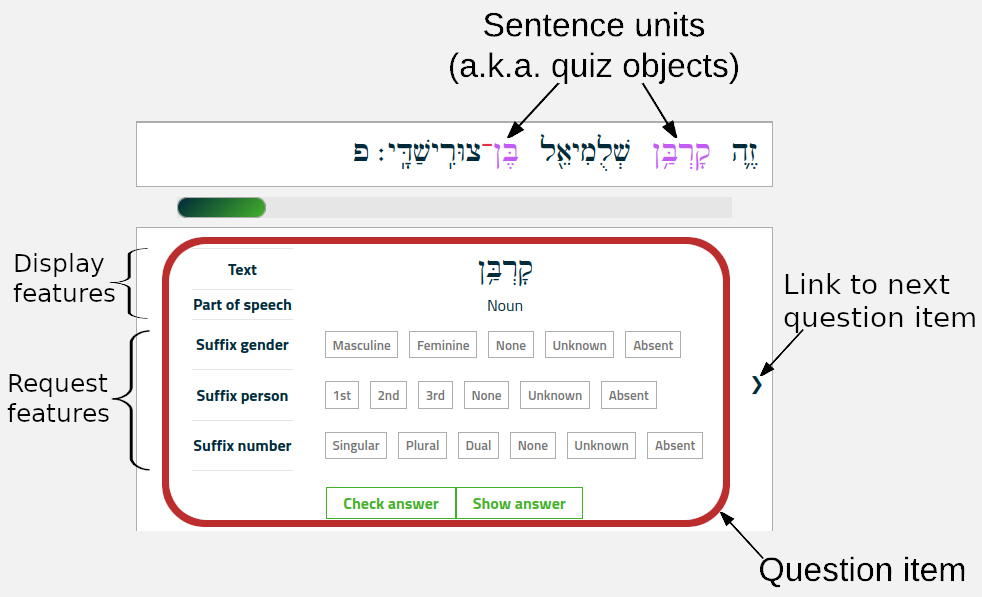
\includegraphics[width=\textwidth]{questionwindow.png}
\caption{A question\index{question} containing two question item\index{question item}s.}\label{fig-question}
\end{figure}

\begin{figure}[h]
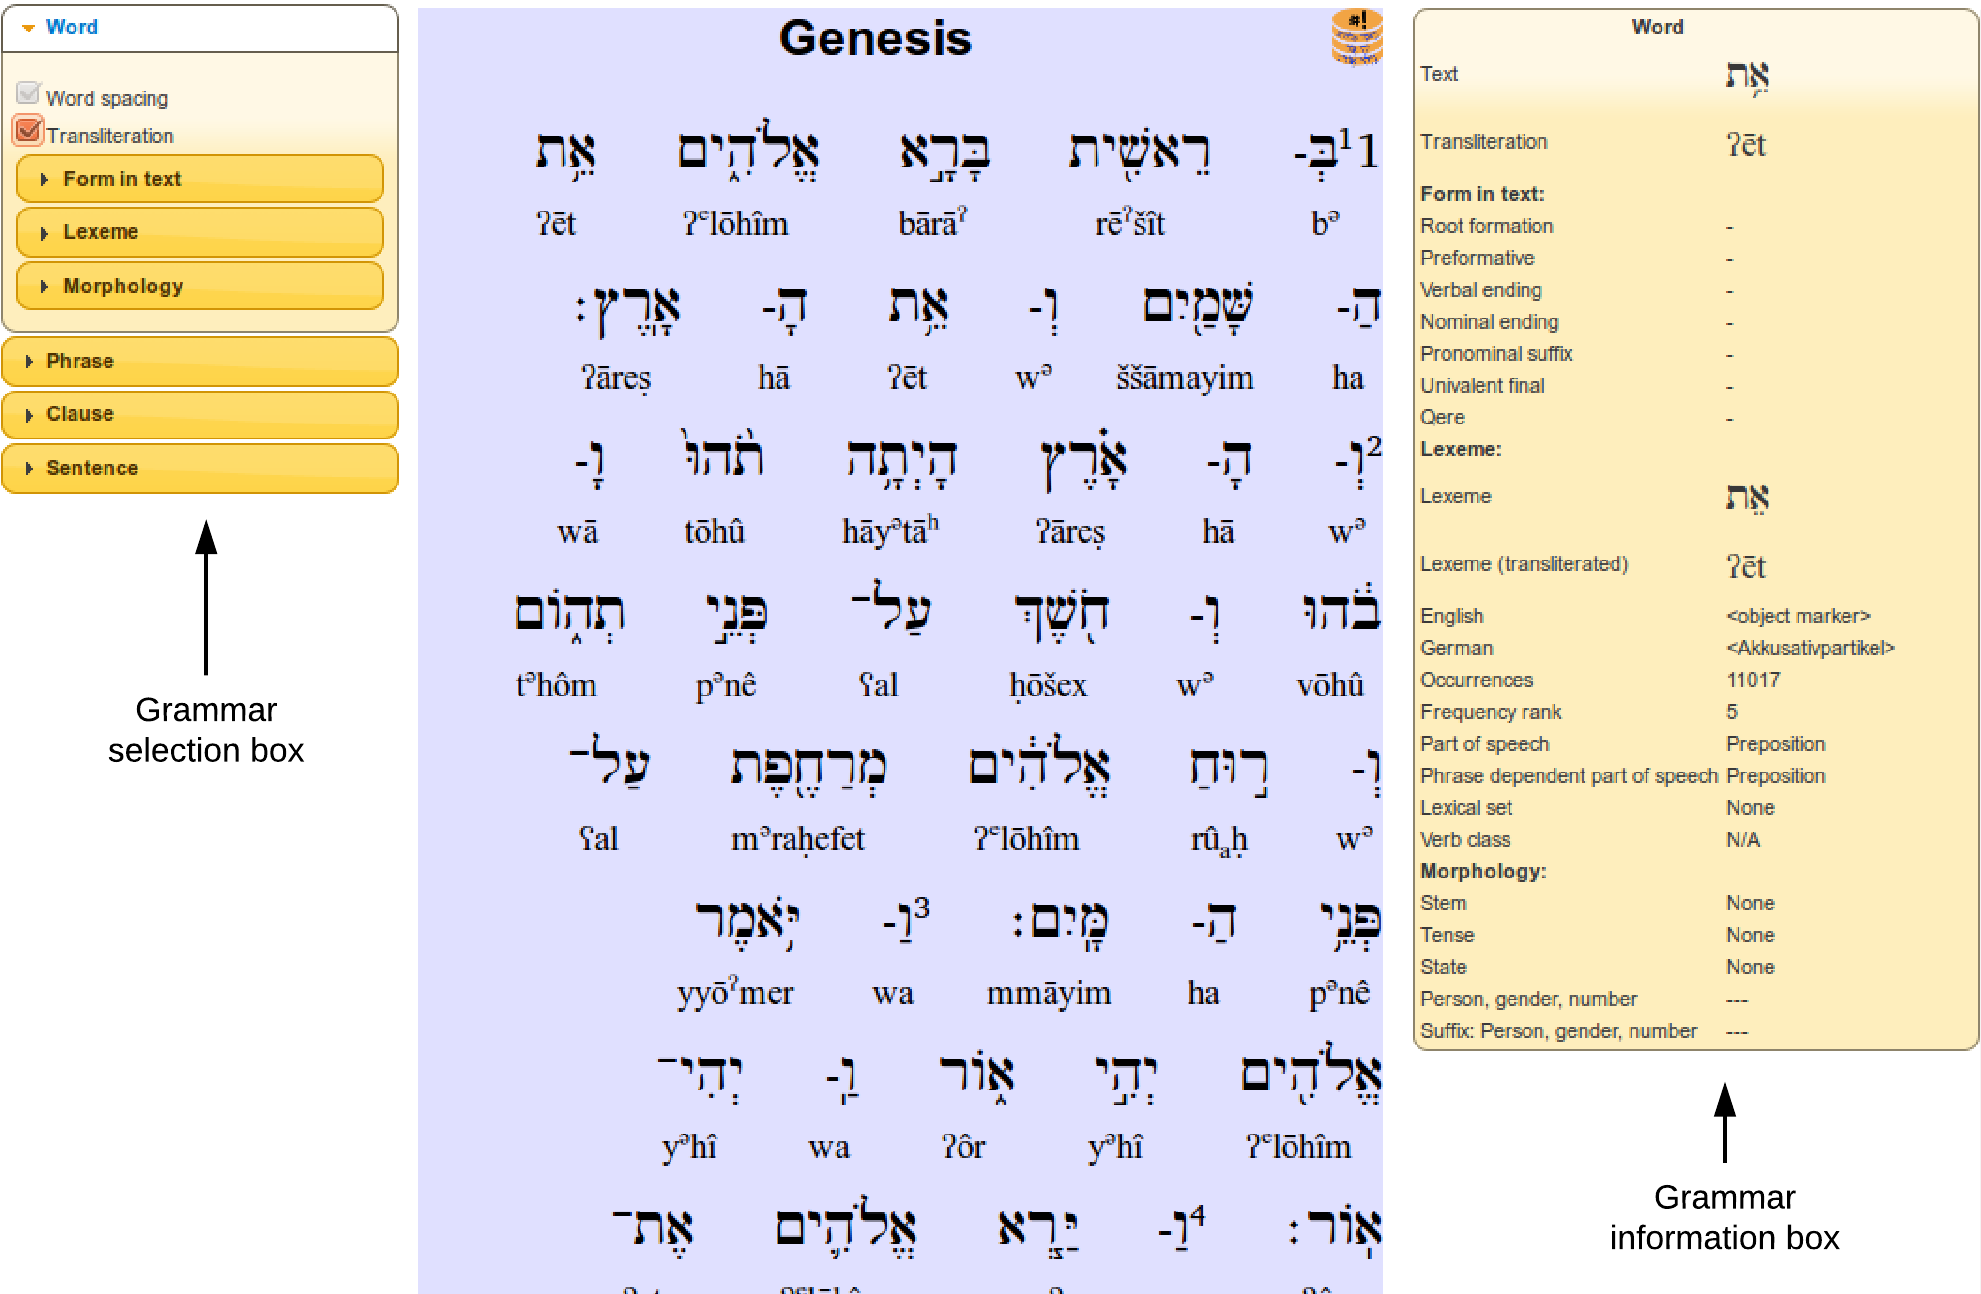
\includegraphics[width=\textwidth]{grammarboxes.png}
\caption{The grammar selection box\index{grammar selection box} and
  the grammar information box\index{grammar information box}.}\label{fig-grammar-info}
\end{figure}


%%%%%%%%%%%%%%%%%%%%%%%%%%%%%%%%%%%%%%%%%%%%%%%%%
%%%%%%%%%%%%%%%%%%%% History %%%%%%%%%%%%%%%%%%%%
\chapter{History}

\textbf{Read this chapter if you want to.}
\plainbreak{3}


%%%%%%%%%%%%%%%%%%%% EQG: A Java Applet (2008) %%%%%%%%%%%%%%%%%%%%
\section{EQG: A Java Applet (2008)}

In 2008 professor Nicolai Winther-Nielsen\index{Winther-Nielsen, Nicolai} told me about a text
database system, Emdros, developed by Ulrik Sandborg-Petersen\index{Sandborg-Petersen, Ulrik}.
Nicolai was teaching Biblical Hebrew at what was then the Copenhagen School of
Theology.\footnote{A.k.a. Dansk Bibel-Institut. This later became the Fjellhaug International
  University College Denmark.}

I further learned that Emdros databases exist with the entire text of the Bible in the original
languages, complete with grammatical information about every single word.

We discussed how these tools could be used by Nicolai in his teaching, and in the autumn of 2008 the
first version of \emph{EQG,} the \emph{Emdros-based Quiz Generator}, was demonstrated, running as a Java
applet in a web browser.

%%%%%%%%%%%%%%%%%%%% 3ET: A Stand-alone Java Program (2009-2010) %%%%%%%%%%%%%%%%%%%%
\section{3ET\index{3ET}: A Stand-alone Java Program (2009-2010)}

The Java applet solution was not practical, especially since there was no easy way to access an
Emdros database over a network connection. In 2009 the applet was therefore abandoned in favour of a
stand-alone PC application, still written in Java but running directly under Microsoft Windows.

The name was changed to \emph{3ET,} \emph{Ezer's Emdros-based Exercise Tool}, and an attempt was made to
market it through 3BM, a company owned by Nicolai and his colleague Jens Bruun Kofoed%
\index{Kofoed, Jens Bruun}.

The name 3ET is still reflected in the file extension \texttt{.3et}\index{.3et (file extension)}
used in quiz template files.

%%%%%%%%%%%%%%%%%%%% PLOTLearner: A EuroPLOT Product (2011-2013) %%%%%%%%%%%%%%%%%%%%
\section{PLOTLearner\index{PLOTLearner}: A EuroPLOT Product (2011-2013)}

In 2011 3ET became part of an EU project about \emph{Persuasive Learning Objects and Technologies},
PLOT. The project became known as EuroPLOT\index{EuroPLOT},\footnote{\url{http://www.eplot.eu}.} and
3ET changed its name to \emph{PLOTLearner.}

Since PLOTLearner was part of an EU project the source code was made open under an MIT
License.\footnote{\url{http://opensource.org/licenses/MIT}.} PLOTLearner was the last Java-based
version of the product, and it can be downloaded from
\url{http://eplot.3bmoodle.dk/index.php/downloads}.

%%%%%%%%%%%%%%%%%%%% Bible Online Learner: Web-based (since 2013) %%%%%%%%%%%%%%%%%%%%
\section{Bible Online Learner\index{Bible Online Learner}: Web-based (since 2013)}

Since 2013 the program has been moved from a Java-based stand-alone PC application to a web-based
solution. The name of the product was changed once more and became \emph{Bible Online Learner},
or \emph{Bible OL}\index{Bible OL} for short. This is the product that is described in this document.



%%%%%%%%%%%%%%%%%%%%%%%%%%%%%%%%%%%%%%%%%%%%%%%%%%%%%%%%%%%%%
%%%%%%%%%%%%%%%%%%%% Installing Bible OL %%%%%%%%%%%%%%%%%%%%
\chapter{Installing\index{installation} Bible OL}\label{chap-install}

\textbf{Read as much of this chapter as you find necessary.}
\plainbreak{3}

This chapter describes how to install Bible OL on a computer. What you need to do, depends on what
you mean by ``installing'' Bible OL. If you want to set up a server that runs Bible OL for the
benefit of researchers and students, follow the instructions in Section \ref{sec-host}.
If you want to get your own copy of Bible OL in order to enhance or modify it, follow the
instructions in Section \ref{sec-devel}.


%%%%%%%%%%%%%%%%%%%% Hosting Bible OL %%%%%%%%%%%%%%%%%%%%
\section{Hosting\index{hosting} Bible OL}\label{sec-host}

Bible OL runs on a Linux\index{Linux} server. I'm sure that it would be quite easy to host it on a
Mac\index{Mac} or a Windows\index{Windows} computer, but I haven't tried this myself, and the
following instructions are aimed at people with a computer running the Linux operating system.

\subsection{Step 1. Server Software}

The following software must be installed on your server (please pay attention to the PHP version number):

\begin{itemize}
\item Apache\index{Apache} (web server\index{web server}). I use version 2.4.18, but version 2.2.22 also works.
\item MySQL\index{MySQL} (database system). I use version 5.7.21.
\item SQLite3\index{SQLite3} (database system used by Emdros). I use version 3.11.0.
\item PHP\index{PHP}. I use version 7.1.
\item git\index{Git}. I use version 2.7.4.
\end{itemize}

All of this can be installed on an Ubuntu Linux system using the usual \emph{apt-get} installation
program. I have not done a thorough investigation into the minimum required versions of these
software packages; you should not see the versions mentioned above as minimum requirements.



\subsection{Step 2. Install Emdros\index{Emdros}}\label{sec-install-emdros}

You must install the Emdros database system. This is probably the most complex part of
the installation process since Emdros is not a standard component in any operating system.

I use Emdros version 3.5.23. Emdros can be downloaded from
\url{https://emdros.org/download.html}.

Follow the instructions that come with Emdros to compile and install it on your computer. You will
need a C++\index{C++} compiler and the Gnu make%
\index{make}\index{Gnu make|see {make}}\index{gmake|see {make}}
system (and probably a few other things as well -- check the Emdros documentation).

When you compile Emdros, be sure to include support for PHP~7\index{PHP}. I use this
\emph{configure}\index{configure} command to set up the Emdros compilation:

% Do not set language=bash in the following line lest "local" be printed in blue
\begin{lstlisting}
./configure --with-sqlite3=local --with-mysql=yes --with-default-backend=sqlite3 \
    --with-swig-language-php=yes --with-swig-language-java=no --with-swig-language-python=no \
    --with-swig-language-perl=no --with-wx=no --with-swig-language-ruby=no \
    --with-swig-language-php7=yes --with-swig-language-nodejs=no
\end{lstlisting}

If you want to include support for other programming languages, you
will need to change this command.

When you have compiled and installed Emdros (using the ``make'' and ``sudo make install'' commands,
respectively) you need to enable access to Emdros in PHP. The correct way to do this depends on your
Apache\index{Apache} and PHP installation. In my case, I had to copy the file
\texttt{EmdrosPHP7.ini} to the directory \texttt{/etc/php/7.1/mods-available} and then run the
command

\begin{lstlisting}[language=bash]
  sudo phpenmod -v 7.1 EmdrosPHP7
  sudo service apache2 restart
\end{lstlisting}

If you cannot or do not want to enhance PHP with Emdros support, you can configure Bible OL to use
the \emph{mql}\index{MQL} command line tool instead, but this is not recommended. More information
about that is given in Section \ref{sec-mql-extern}.

If you already have Emdros installed on a development system, and if your runtime system uses the
same operating system as your development system, you can simply copy the Emdros files to your
runtime systems. The files to copy will be typically found in \texttt{/usr/local/bin} and
\texttt{/usr/local/lib/emdros}. (I have never actually done this, and I suspect that you may need to
run \emph{ldconfig}\index{ldconfig} after copying the files to your runtime system.)


\subsection{Step 3. Download Bible OL}\label{sec-download-bol}\index{download Bible OL}

You can download Bible OL from GitHub\index{GitHub} using these commands:

\begin{lstlisting}[language=bash]
cd %\textrm{\emph{installation directory}}%
git clone --recursive https://github.com/EzerIT/BibleOL
\end{lstlisting}\index{clone|hyperit}

This will fetch all the Bible OL software, including five submodules needed by Bible OL. The
\emph{git}\index{Git} command will create a directory called \texttt{BibleOL} under the current directory.

\emph{Note:} If you have forked\index{fork GitHub} Bible OL on GitHub you should replace the URL in the ``git clone''
command above with a URL that points to your repository on GitHub. (See section
\ref{sec-fork-github} for more information.)

When the download completes, execute the following commands:

\begin{lstlisting}[language=bash]
cd BibleOL
git-hooks/setup.sh
\end{lstlisting}

This will install a Git hook\index{hook, Git} that automatically downloads the necessary databases
from Dropbox\index{Dropbox} when needed.


\subsection{Step 4. Configure MySQL\index{MySQL}}\label{sec-database-php}

Create an empty database\index{user database}\index{database, user|see {user database}} in MySQL. Then copy the file
\texttt{myapp/config/database.php-dist} to \texttt{myapp/config/database.php} and modify the
following lines in the copy:

\begin{lstlisting}[language=PHP]
'username' => 'USERNAME',
'password' => 'PASSWORD',
'database' => 'DATABASE',
\end{lstlisting}

Change the text USERNAME, PASSWORD, and DATABASE to be the database username, password, and database
name.


\subsection{Step 5. Additional Configuration}

Copy the file \texttt{myapp/config/ol.php-dist} to \texttt{myapp/config/ol.php}\index{ol.php} and modify the
following lines in the copy:

\begin{lstlisting}[language=PHP]
$config['variants'] = array();

$config['pw_salt'] = 'xxxxxxx';
$config['mql_driver'] = 'native';
$config['mail_sender_address'] = 'xxxxx@xxxxx.xx';
$config['mail_sender_name'] = 'Bible Online Learner';

$config['google_login_enabled'] = false;
$config['google_client_id'] = 'xxxxxxxxxxxx.apps.googleusercontent.com';
$config['google_client_secret'] = 'xxxxxxxxxxxxxxxxxxxxxxxx';

$config['facebook_login_enabled'] = false;
$config['facebook_client_id'] = 'xxxxxxxxxxxxxxxx';
$config['facebook_client_secret'] = 'xxxxxxxxxxxxxxxxxxxxxxxxxxxxxxxx';
\end{lstlisting}

You should modify these values thus:

\begin{my-longtabu}{>{\footnotesize\ttfamily}lX}{ \headii{\normalsize\textrm{Variable}}{Contents} }
\$config['variants']\index{variants} & An array of strings. This array must contain the names of all the
language variants (see Section \ref{sec-variants}) that Bible OL should provide. The variant names should
consist of only letters and digits. (Note: Whenever this value is changed, Bible OL will be quite slow the
first time a biblical text is displayed. This is because the system creates database tables for the added variants.)\\

\$config['pw\_salt']\index{salt} & A random text string of, say, 6-8 characters. This is used to randomize the
  user passwords stored in the user database\index{user database}.\\

\$config['mql\_driver']\index{MQL driver}\index{driver, MQL|see {MQL driver}} & Set to \texttt{'native'} to select a
built-in MQL driver. Set to or \texttt{'extern'} to run MQL commands external to the PHP interpreter
(see Section \ref{sec-mql-extern}).\\

\$config['mail\_sender\_address']\index{email address}\index{address|see {email address}} & The email address to
be used as sender when Bible OL sends email to users.\\

\$config['mail\_sender\_name']\index{email sender}\index{sender|see {email sender}} & The name to be used as
sender when Bible OL sends email to users.\\

\$config['google\_login\_enabled']\index{login!Google}\index{Google!login|see {login, Google}} & Set to \emph{true} if
you have a Google apps account\index{Google!apps account} that allows you to service Google logins;
set to \emph{false} to disable Google login.\\

\$config['google\_client\_id']\index{Google!client ID}\index{client ID|see {Google, client ID}} & Your Google apps
client ID. Used only if you enable Google login.\\

\$config['google\_client\_secret']\index{Google!client secret}\index{client secret|see {Google, client secret}} & Your
Google apps client secret, if any. Used only if you enable Google login.\\

\$config['facebook\_login\_enabled']\index{login!Facebook}\index{Facebook!login|see {login, Facebook}} & Set to \emph{true} if
you have a Facebook developers account\index{Facebook!developers account} that allows you to service Facebook logins;
set to \emph{false} to disable Facebook login.\\

\$config['facebook\_client\_id']\index{Facebook!app ID}\index{app ID|see {Facebook, app ID}} & Your Facebook app
ID. Used only if you enable Facebook login.\\

\$config['facebook\_client\_secret']\index{Facebook!app secret}\index{app secret|see {Facebook, app secret}} & Your
Facebook app secret. Used only if you enable Facebook login.\\
  
\end{my-longtabu}

Copy the file \texttt{myapp/config/config.php-dist} to \texttt{myapp/config/config.php} and modify the
following line in the copy:

\begin{lstlisting}[language=PHP]
$config['base_url'] = 'http://example.com';%\index{base URL}%
$config['lj_enabled'] = false;
\end{lstlisting}

Replace `http://example.com' with the top URL of the web site for your Bible OL installation.

If you plan to use \emph{Learning Journey} (see Section \ref{sec-lj}), set \texttt{\$config['lj\_enabled']} to \texttt{true}.


\subsection{Step 6. Initialize MySQL\index{MySQL}}

The following commands should be executed with the current directory set to \texttt{BibleOl}.

\subsubsection*{Substep 1}

Initialize the contents of the database from the content of the file \texttt{bolsetup.sql}.

If you plan to use \emph{Learning Journey} (see Section \ref{sec-lj}), you may also want to import
the content of the file \texttt{ljsetup.sql}.


\subsubsection*{Substep 2}

Populate the database with the available translations by issuing this command:

\begin{lstlisting}[language=bash]
./setup_lang.sh
\end{lstlisting}

(On my computer, this takes a couple of minutes.)


\subsection{Step 7. Add Administrator\index{administrator}}

You must manually add an administrator to the MySQL database. You do this by adding an entry to the
table \emph{bol\_user}\index{bol\_user table|see {user table}}\index{user table} (see Section \ref{sec-user-table}).
The entry should have the \emph{isadmin} field set to 1 (\emph{true}). The
\emph{password}\index{password} should be set to the value of this PHP function:

\begin{lstlisting}[language=PHP]
md5($config['pw_salt'] . 'xxxxx');%\index{md5}%
\end{lstlisting}

\noindent
where \emph{\$config[\q pw\_salt\q]}\index{salt} is configured in \texttt{myapp/config/ol.php}, and
\emph{xxxxx} is the user's desired password.

You can also find the correct value of the password by executing this shell command:

\begin{lstlisting}[language=bash]
echo -n sssssxxxxx | md5sum%\index{md5sum}%
\end{lstlisting}

\noindent
where \emph{sssss} is the value of \emph{\$config[\q pw\_salt\q]} and \emph{xxxxx} is the user's
desired password.


\subsection{Step 8. Apache Configuration}\index{Apache!Configuration}

Set up the Apache web server to access Bible OL. Make sure that Apache is configured to allow
\texttt{.htaccess}\index{htaccess@.htaccess} files. This is controlled by the Apache
\emph{AllowOverride}\index{AllowOverride, Apache directive} directive.

Copy the file \texttt{.htaccess-dist} to \texttt{.htaccess} and modify the following line in the
copy:

\begin{lstlisting}
RewriteBase /%\index{RewriteBase, Apache directive}%
\end{lstlisting}

The correct value here depends on your Apache configuration. If your web server is set up to serve
Bible OL at the url \texttt{http://example.com/alpha/beta}, then the above line should be changed to:

\begin{lstlisting}
RewriteBase /alpha/beta%\index{RewriteBase, Apache directive}%
\end{lstlisting}

If you have a dedicated hostname for Bible OL (for example, \texttt{http://example.com}), you should
leave \emph{RewriteBase} as it is: a single slash.

\subsection{Step 9. Set Up Quiz Template Directory}

Create a directory called \texttt{quizzes} in the installation directory. Quiz template files will
be stored here. If you want to, you can copy the contents of the \texttt{quiz\_templates} directory,
which contains sample quiz templates, to \texttt{quizzes}.

Make sure that the permissions on the \texttt{quizzes} directory and its contents is set to allow
the web server to modify the files.

\subsection{Step 10. Additional PHP Configuration}\index{PHP!Configuration}

Unfortunately, the default PHP configuration on some Linux distributions has problems with login
session timeouts. This affects the system session folder\index{PHP!system session folder} and the session garbage
collection probability\index{PHP!garbage collection}.

Depending on your Linux distribution, you may have to perform the following steps:

The system session folder is probably \texttt{/var/lib/php/sessions}. This folder must be owned by
the Apache web server (that is probably user \emph{www-data}). In order to fix this, issue the
following commands:

\begin{lstlisting}[language=bash]
sudo chown www-data:www-data /var/lib/php/sessions
ls -ld /var/lib/php/sessions
\end{lstlisting}

These commands should produce this output (the time stamp and file size may differ):

\begin{lstlisting}
drwx-wx-wt 2 www-data www-data 32768 jul  1 11:02 /var/lib/php/sessions
\end{lstlisting}


The garbage collection probability is controlled by the configuration variables
\emph{session.gc\_probability} and \emph{session.gc\_divisor}. As superuser, you must edit the PHP
configuration file \texttt{/etc/php/7.2/apache2/php.ini} (where 7.2 should be replaced by your PHP
version number). In that file you must ensure that the configuration variables have these values:

\begin{lstlisting}
session.gc_probability = 1
session.gc_divisor = 100
\end{lstlisting}

After making these changes, reload the Apache configuration; for example, thus:

\begin{lstlisting}[language=bash]
sudo service apache2 reload
\end{lstlisting}




%%%%%%%%%%%%%%%%%%%% Bible OL Development System Setup %%%%%%%%%%%%%%%%%%%%
\section{Bible OL Development\index{development} System Setup}\label{sec-devel}

This section describes how to set up a complete development system for working with all aspects of
Bible OL development. Depending on the type of development you are going to do, you may not need all
of this.

You may want to read Chapter \ref{chap-proglang} before you proceed with the following.

Section \ref{sec-download-bol} describes how to download Bible OL. If you plan to make any
modifications to the software, I recommend that you fork\index{fork GitHub} Bible OL on GitHub
before downloading it. See section \ref{sec-fork-github} for more information.

If you want to test Bible OL on your own computer, you should also set it up as a Bible OL server.
Please see Section \ref{sec-host} for information about how to do this.

Much of the description here is quite vague. In many cases I am simply describing what \emph{I} have
done. Your system may be different, and you may need to do things I have not described.

For Bible OL, I use a computer with the Linux\index{Linux} operating system (the
Ubuntu\index{Ubuntu} distribution). I am sure the system could also be set up on a
Windows\index{Windows} or Mac\index{Mac} computer, but I have not tried it and you will not find any
instructions how to do it here.

The following should be installed:

\begin{itemize}
\item SQLite3\index{SQLite3} (database system used by Emdros). I use version 3.11.0.
\item PHP\index{PHP}. I use version 7.1.
\item nodejs\index{nodejs} (JavaScript runtime, used for compiling TypeScript and Less). I use version
  4.2.6.
\item npm\index{npm} (package manager for nodejs). I use version 3.5.2.
  This package may not strictly be required, but it is useful for installing nodejs modules.
\item git\index{Git}. I use version 2.7.4.
\end{itemize}

All of this can be installed on an Ubuntu system using the usual \emph{apt-get} installation
program. I have not done a thorough investigation into the minimum required versions of these
software packages; you should not see the versions mentioned above as minimum requirements.

You will also need to install the Emdros database system, a Less compiler, and a TypeScript
compiler. This is detailed in Sections \ref{sec-install-start}-\ref{sec-install-end}.

\subsection{Forking\index{fork GitHub} Bible OL on GitHub\index{GitHub}}\label{sec-fork-github}

If you plan to make any modifications to the software, I recommend that you fork Bible OL on GitHub
before downloading it. In order to do this you must set up an account on \url{https://github.com}.
After this, navigate to \url{https://github.com/EzerIT/BibleOL} and click the ``Fork'' label in the
upper right section of the web page.

Please note that this document is not a manual on how to use Git and GitHub. You are expected to
know this.

Section \ref{sec-download-bol} tells you how to download Bible OL from the original repository. To
download from your own fork, you should use these commands:


\begin{lstlisting}[language=bash]
cd %\textrm{\emph{installation directory}}%
git clone --recursive https://github.com/%\textrm{\emph{username}}%/BibleOL
\end{lstlisting}\index{clone}

\noindent
or

\begin{lstlisting}[language=bash]
cd %\textrm{\emph{installation directory}}%
git clone --recursive git@github.com:%\textrm{\emph{username}}%/BibleOL.git
\end{lstlisting}\index{clone}

\noindent
depending on which way you prefer to access GitHub. (Replace \emph{username} in the commands above
with your GitHub username.)

In either case, remember to execute these commands:

\begin{lstlisting}[language=bash]
cd BibleOL
git-hooks/setup.sh
\end{lstlisting}

\noindent
as described in Section \ref{sec-download-bol}.

Bible OL uses a number of Git submodules: ckeditor, zocial, jstree, and
virtualkeyboard. The \mbox{``-\thinspace-recursive''} flag in the ``git clone'' command causes these submodules to be
cloned from the ``EzerIT'' repository. You may want to replace them with your own copies of the
repositories. The following table lists their names and their location on GitHub:

\begin{my-tabu}{lll}{ \headiii{Submodule}{My forked location}{Original location} }
ckeditor         \index{ckeditor}        & EzerIT/ckeditor-releases   & ckeditor/ckeditor-releases \\
zocial           \index{zocial}          & EzerIT/css-social-buttons  & samcollins/css-social-buttons \\
jstree           \index{jstree}          & EzerIT/jstree              & vakata/jstree \\
virtualkeyboard  \index{virtualkeyboard} & EzerIT/virtualkeyboard     & \emph{Not on GitHub} \\
\end{my-tabu}

Previous versions of Bible OL also used submodules called CodeIgniter and bootstrap. They are no longer
submodules but an integrated part of the Bible OL software tree; they are located in the directories
\texttt{CodeIgniter\_Local} and \texttt{bootstrap\_local}, respectively.

\subsection{Installing Emdros\index{Emdros!installation}}\label{sec-install-start}
 
In order to install Emdros, you should follow the instructions given in in Section
\ref{sec-install-emdros}.
 
 
\subsection{Installing Lessc\index{lessc!installation}}\label{sec-installing-lessc}
 
\emph{Lessc}\index{lessc} is the Less\index{Less} compiler. It runs under \emph{nodejs}\index{nodejs}, which is
a stand-alone JavaScript\index{JavaScript} runtime system.

For information about how to use the Less compiler, see \url{http://lesscss.org}.

The \emph{lessc} command can be installed using this shell command:
 
\begin{lstlisting}[language=bash]
sudo npm install -g less
\end{lstlisting}
 
The ``-g'' option means the software is installed globally and can be used by all users of the
computer. Alternatively, the ``-g'' option and the ``sudo'' can be omitted, which will install
\emph{lessc} only for the local user; but in that case the \emph{lessc} command must be executed using
the pathname \mbox{\emph{\textasciitilde/node\_modules/.bin/lessc}}.
 
I use version 3.0.1 of \emph{lessc}.

\subsection{Installing Tsc\index{tsc!installation}\index{TypeScript!compiler|see {tsc}}}\label{sec-installing-tsc}\label{sec-install-end}
 
\emph{Tsc}\index{tsc} is the TypeScript\index{TypeScript} compiler. It
runs under \emph{nodejs},\index{nodejs} which is a stand-alone JavaScript\index{JavaScript} runtime
system. For information about how to use the TypeScript compiler, see
\url{http://www.typescriptlang.org}.

The \emph{tsc} command can be installed using these shell commands:
 
\begin{lstlisting}[language=bash]
sudo npm install -g typescript
npm install @types/bootstrap @types/jquery @types/jqueryui
\end{lstlisting}

The ``-g'' option means the software is installed globally and can be used by all users of the
computer. Alternatively, the ``-g'' option and the ``sudo'' can be omitted, which will install
typescript only for the local user; but in that case the \emph{tsc} command must be executed using
the pathname \mbox{\emph{\textasciitilde/node\_modules/.bin/tsc}}.

Note that there is no ``sudo'' and no ``-g'' option on the second ``npm'' command.

I use version 3.2.2 of \emph{tsc}.

Note: If you are building an older version of Bible OL (that is, on in which the file
\mbox{\emph{ts/jquery/jquery.d.ts}} exists), you must not install the modules \emph{@types/bootstrap,
  @types/jquery,} and \emph{@types/jqueryui} mentioned above.


%%%%%%%%%%%%%%%%%%%%%%%%%%%%%%%%%%%%%%%%%%%%%%%%%%%%%%%%%%%%%%%%%%%%%%%%%%%%%%
%%%%%%%%%%%%%%%%%%%% Programming Languages and Frameworks %%%%%%%%%%%%%%%%%%%%
\chapter{Programming Languages and Frameworks}\label{chap-proglang}

\textbf{As a developer, you must read this chapter.}
\plainbreak{3}

A considerable number of programming languages and other specification languages are used in the
creation and execution of Bible OL. This chapter gives a brief overview of these languages and
points you to where you may learn more about them.


%%%%%%%%%%%%%%%%%%%% PHP %%%%%%%%%%%%%%%%%%%%
\section{PHP}\index{PHP|hyperit}

The main language used on the server side is PHP\footnote{\url{http://php.net}.}, which is a popular
general-purpose scripting language that is especially suited to web development.

In order to execute Bible OL, the PHP implementation on the server must be enhanced with features to
execute MQL commands. This is described in Section \ref{sec-install-emdros}.

%%%%%%%%%%%%%%%%%%%% CodeIgniter %%%%%%%%%%%%%%%%%%%%
\section{CodeIgniter}\label{sec-codeigniter}\index{CodeIgniter}

Bible OL uses a PHP framework known as \emph{CodeIgniter.}\footnote{\url{http://www.codeigniter.com}.}
More information about this is given in Chapter \ref{chap-codeigniter-use}.


%%%%%%%%%%%%%%%%%%%% SQL %%%%%%%%%%%%%%%%%%%%
\section{SQL}\index{SQL|hyperit}

SQL\footnote{See \url{https://en.wikipedia.org/wiki/SQL}.} is a language for manipulating a
relational database. Bible OL uses the MySQL database\footnote{\url{http://www.mysql.com}.} system to store
information about users who have an account on the Bible OL website. Bible OL uses the SQLite3
database system to store the ``Words Database'' (see chapter \ref{chap-multiple-choice}) and the
``Hints Database'' (see Chapter \ref{chap-hints}).

SQL commands are executed from PHP code through CodeIgniter.


%%%%%%%%%%%%%%%%%%%% MQL %%%%%%%%%%%%%%%%%%%%
\section{MQL}\label{sec-mql}\index{MQL}

MQL is a language for manipulating Emdros\index{Emdros}\footnote{\url{http://emdros.org}.} text
databases. The PHP implementation on the server must be extended with function to execute MQL
commands. This is described in Section \ref{sec-install-emdros}.

MQL and Emdros are described in greater detail in Chapter \ref{chap-emdros-use}.



%%%%%%%%%%%%%%%%%%%% HTML %%%%%%%%%%%%%%%%%%%%
\section{HTML}\index{HTML|hyperit}

The generated web pages use HTML version 5.\footnote{See \url{https://en.wikipedia.org/wiki/HTML5}.}


%%%%%%%%%%%%%%%%%%%% CSS %%%%%%%%%%%%%%%%%%%%
\section{CSS}\label{sec-css}\index{CSS|hyperit}

CSS (Cascading Style Sheets)\footnote{See
  \url{https://en.wikipedia.org/wiki/Cascading_Style_Sheets}} is a language for specifying the
layout style of a web page. However, only a small part of the Bible OL styles are written directly
in CSS. Most styling is written in Less which is then compiled into CSS.


%%%%%%%%%%%%%%%%%%%% Less %%%%%%%%%%%%%%%%%%%%
\section{Less}\label{sec-less}\index{Less}

Less\footnote{\url{http://lesscss.org}.} is a CSS pre-processor, meaning that it
extends the CSS language, adding features that allow variables, mixins, functions and many other
techniques that allow you to make CSS that is more maintainable, themable and extendable.

Although Less style files can be compiled when used in a browser, the Bible OL implementation
compiles Less files only once and stores the resulting CSS files.

More information about how Less is used is given in Chapter \ref{chap-less-use}.

%%%%%%%%%%%%%%%%%%%% JavaScript %%%%%%%%%%%%%%%%%%%%
\section{JavaScript}\index{JavaScript|hyperit}

On the client side (that is, in the user's browser) the software is loaded as
JavaScript\footnote{See \url{https://developer.mozilla.org/en-US/docs/Web/JavaScript}.} code.
However, only a small part of Bible OL is written directly in JavaScript. Most client-side software
is written in TypeScript which is then compiled into JavaScript.

%%%%%%%%%%%%%%%%%%%% TypeScript %%%%%%%%%%%%%%%%%%%%
\section{TypeScript}\label{sec-typescript}\index{TypeScript}

TypeScript\footnote{\url{http://www.typescriptlang.org}.} is a superset of JavaScript that adds
strong typing and proper classes to JavaScript.

Most of the client-side software of Bible OL is written in TypeScript which is then compiled into
JavaScript.

More information about how TypeScript is used is given in Section
\ref{sec-typescript-use}.

%%%%%%%%%%%%%%%%%%%% JSON %%%%%%%%%%%%%%%%%%%%
\section{JSON}\index{JSON|hyperit}

JSON\footnote{\url{http://json.org}.} is a text-based data-interchange format. It is used to
transfer data between the server and the client.

%%%%%%%%%%%%%%%%%%%% jQuery and jQuery UI %%%%%%%%%%%%%%%%%%%%
\section{jQuery and jQuery UI}\index{jQuery|hyperit}\index{jQuery UI|hyperit}

On the client side Bible OL uses a JavaScript/TypeScript framework known as
\emph{jQuery}\footnote{\url{https://jquery.com}.} and its associate user interface functions
\emph{jQuery UI.}\footnote{\url{https://jqueryui.com}.}

%%%%%%%%%%%%%%%%%%%% Bootstrap %%%%%%%%%%%%%%%%%%%%
\section{Bootstrap}\index{Bootstrap|hyperit}

On the client side Bible OL uses a JavaScript framework known as
\emph{Bootstrap.}\footnote{\url{https://getbootstrap.com}.} Currently, Bible OL uses Bootstrap
version 4.1.2.

%%%%%%%%%%%%%%%%%%%% RGraph %%%%%%%%%%%%%%%%%%%%
\section{RGraph}\index{RGraph|hyperit}

Bible OL can display graphs showing statistics about how students are doing. The graphs are
constructed using \emph{RGraph.}\footnote{\url{https://www.rgraph.net}.} Currently, Bible OL uses
RGraph version 4.63.


%%%%%%%%%%%%%%%%%%%% What You Must Know %%%%%%%%%%%%%%%%%%%%
\section{What You Must Know}

If you plan to modify the Bible OL server-side code, you must know how to program in PHP, and you
must understand the CodeIgniter framework. You may also need to have a good understanding of HTML,
Less, CSS, SQL, MQL, and JSON.

If you plan to modify the Bible OL client-side code, you must know how to program in TypeScript, and
you must understand the jQuery framework, the Bootstrap framework, and, perhaps, the jQuery UI
functions. You may also need to have a good understanding of HTML, CSS, JavaScript, and JSON.

Obviously, you also need a good understanding of how Bible OL works from a user's perspective.


%%%%%%%%%%%%%%%%%%%%%%%%%%%%%%%%%%%%%%%%%%%%%%%%%%%%%%%%%%%%%%%%%%%%%%%%
%%%%%%%%%%%%%%%%%%%% High-level System Architecture %%%%%%%%%%%%%%%%%%%%
\chapter{High-level System Architecture}\index{architecture}\index{system architecture|see {architecture}}

\textbf{As a developer, you must read this chapter.}

\plainbreak{3}

Bible OL consists of two main components, the server\index{server|hyperit} and the
client\index{client|hyperit}, as shown in the following illustration.

\begin{center}
  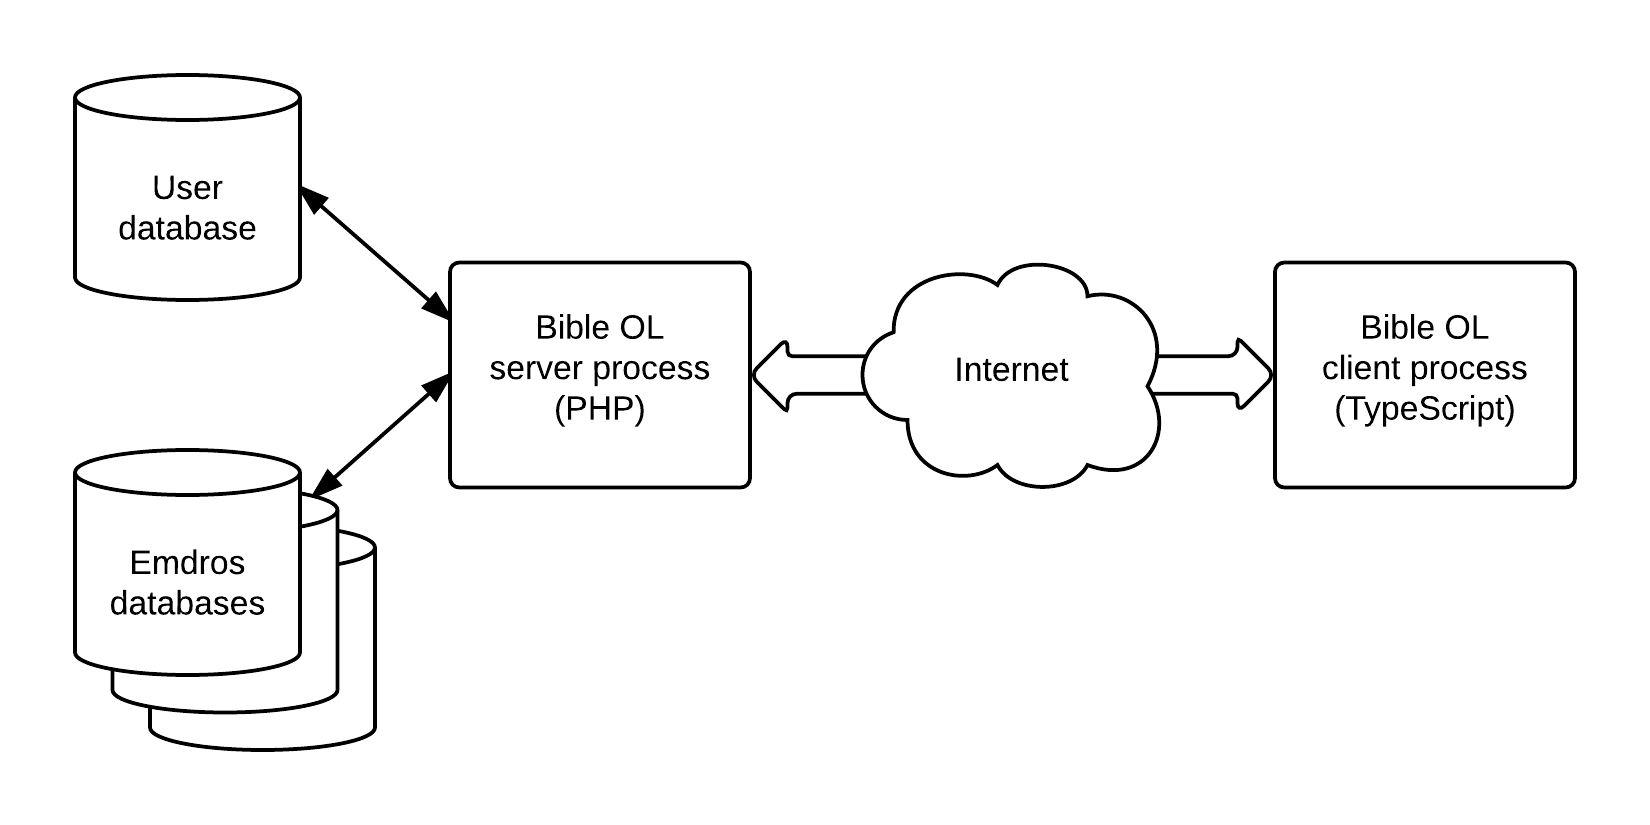
\includegraphics[width=0.9\textwidth]{BOL_overview.png}
\end{center}

The server process runs on a Linux computer, but can probably quite easily be ported to a Windows server
that supports PHP, MySQL, and Emdros. It is programmed in PHP\index{PHP} and has access to a number of
databases:

\begin{itemize}
\item The user database\index{user database} which contains information about registered users and
  translations of Bible OL into various languages.\footnote{The term ``user database'' is thus
    somewhat misleading, but the name is retained in this document, nevertheless.}
\item A number of Emdros databases, which contain the text and grammatical information for the Old
  and New Testaments (and potentially other texts as well).
\end{itemize}

The client is a web browser\index{web browser}\index{browser|see {web browser}} that accesses the server over an
internet connection. It requests the server to provide an exercise or a portion of a text, which it
then displays in the browser window. The client code is primarily written in
TypeScript\index{TypeScript}, which has been translated to JavaScript\index{JavaScript} so that the
browser can execute it.

Most of the layout is done in the client. The server generates HTML code for the main items in the
window, but the actual text to be displayed is stored in variables in the client code, and the layout of
this information is performed by the client.

The data exchange between the client and the server is either a two-step or a three-step exchange.
If the client merely requests a text to be displayed, the data exchange is:

\begin{enumerate}
\item The client requests the server to load a particular URL. The text to display is coded into
  this URL.
\item The server sends the requested text to the client.
\end{enumerate}

If the client requests an exercise to be displayed, the data exchange is:

\begin{enumerate}
\item The client requests the server to load a particular URL. The URL contains information about which
  quiz template to use and how many questions to generate.
\item The server sends the requested exercise to the client.
\item When the user clicks on the``GRADE task''\index{grade task button@``GRADE task'' button}%
  \index{finish button@``Finish'' button|see {``GRADE task'' button}} or ``SAVE
  outcome''\index{save outcome button@``SAVE outcome'' button} button, the client sends the user's
  answers to the server.
\end{enumerate}

Note that there is no data exchange between the client and the server when the user presses the
``Check answer''\index{check answer button@``Check answer'' button} or ``Show answer''%
\index{show answer button@``Show answer'' button}
buttons. These buttons execute code that is local on the server. (This means that in theory a
student can find the correct answers to the questions by looking at the source code for the web
page. This is, however, quite difficult to do, and it is not considered a serious flaw in the design
since it would require considerable knowledge on the part of the student.)


%%%%%%%%%%%%%%%%%%%%%%%%%%%%%%%%%%%%%%%%%%%%%%%%%%%%%%%%%%%%%%
%%%%%%%%%%%%%%%%%%%% Understanding Emdros %%%%%%%%%%%%%%%%%%%%
\chapter{Understanding Emdros}\label{chap-emdros-use}\index{Emdros|hyperit}

\textbf{As a developer, you must read this chapter. If you need to use MQL, you should read the
  whole chapter and also some of the documentation that comes with Emdros.}

\plainbreak{3}

Emdros is a database system for storing and retrieving annotated text. Emdros was developed by Ulrik
Sandborg-Petersen\index{Sandborg-Petersen, Ulrik}. A short introduction to Emdros for linguists is
found at \url{http://emdros.org/petersen-emdros-COLING-2004.pdf}. More documents are available at
\url{http://emdros.org/docs.html}.

Here, only a very brief description of the system will be given. Emdros divides a text into
\emph{objects.}\index{Emdros!object|hyperit} Typical objects are \emph{word, clause,} and
\emph{sentence.} For biblical texts, objects such as \emph{book, chapter,} and \emph{verse} are also
used. Each occurrence of the smallest object, typically a word, is identified by a number, called a
\emph{monad}\index{monad|hyperit} in Emdros terminology.

As an example, consider this text: ``The boy, who had red hair, was sitting on the floor.'' This
sentence consists of 11 words. We can also identify two clauses, ``The boy\ldots was sitting on the
floor'' and ``who had red hair''. Emdros assigns a monad (a positive integer) to each word object:


\begin{center}
  \begin{tabular}{c!{\hspace{1cm}}c}
 
    \begin{tabular}{cc}
      \toprule
      \textbf{Monad} & \textbf{Word}\\
      \midrule
      1 & The  \\
      2 & boy, \\
      3 & who  \\
      4 & had  \\
      5 & red  \\
      6 & hair,\\
      \bottomrule
    \end{tabular}
 
    &
 
    \begin{tabular}{cc}
      \toprule
      \textbf{Monad} & \textbf{Word}\\
      \midrule
      7 & was\\
      8 & sitting\\
      9 & on\\
      10 & the\\
      11 & floor.\\
      &  \\
      \bottomrule
    \end{tabular}
 
  \end{tabular}
\end{center}


Additionally, sets of monads are used to identify clause objects: Monads \{~1-2,~7-11~\} identify
one clause, and monads \{~3-6~\} identify another. Finally, the monads \{~1-11~\} identify a
sentence object.

Associated with each object are a number of \emph{features}%
\index{Emdros!feature|hyperit}\index{feature|see {Emdros, feature}}
that describe various characteristics of the object. For a word object, typical features could be
\emph{part of speech, gender, number, tense,} and \emph{mood.} In the above sentence, word object 4
(the word ``had'') could, for example, have these features:

\begin{my-tabu}{cc}{ \headii{Feature}{Value} }
Text           & ``had''\\
Part of speech & Verb\\
Tense          & Past\\
Number         & Singular\\
Person         & 3rd\\
Lexeme         & ``have''\\
\end{my-tabu}


Similarly, the two clause objects could have a feature called \emph{type} with the values
\emph{main} and \emph{subordinate,} respectively.

The exact set of objects and features available in a database is entirely up to the person who
creates the database.

In addition to the monads, Emdros objects can also be identified by an
ID\_D\index{Emdros!ID\_D|hyperit}\index{ID\_D|see {Emdros, ID\_D}}. Like a monad, the ID\_D is an integer, but
every object in the Emdros database has a unique ID\_D. So a single ID\_D may refer to a single word
or a clause or a sentence. In the above example, the word ``who'' with monad 3 may have ID\_D=8, and
the clause ``who had red hair'' with monads \{~3-6~\} may have ID\_D=12.

Emdros comes with a query language, called MQL\index{MQL|hyperit}\footnote{Mini Query Language.
  (Quite a misnomer since this is a very powerful language.)}, that allows a user to search a corpus
for objects with various features. MQL queries can be quite simple, such as ``find all verbs in the
past tense,'' or very complex, such as ``find all sentences containing a singular pronoun, followed
by at most three words, followed by a verb in the present tense, except cases where the verb is
derived from `to be'.''

The exact syntax of MQL queries can be quite arcane and is beyond the scope of this paper, but
examples can be found in \url{http://emdros.org/petersen-emdros-COLING-2004.pdf}.



%%%%%%%%%%%%%%%%%%%%%%%%%%%%%%%%%%%%%%%%%%%%%%%%%%%%%%%%%%%%%%%%%%%
%%%%%%%%%%%%%%%%%%%% Source Code Tree Overview %%%%%%%%%%%%%%%%%%%%
\chapter{Source Code\index{source code} Tree Overview}

\textbf{As a developer, you must read this chapter.}
\plainbreak{3}

The source code contains the following directories (in alphabetical order):

\begin{my-longtabu}{>{\ttfamily}p{3.3cm}X}{ \headii{\textrm{Name}}{Contents} }
bootstrap\_local\index{Bootstrap} & A JavaScript framework used on the client side of Bible OL.

Webpage: \url{https://getbootstrap.com}.

Source: \url{https://github.com/twbs/bootstrap.git}.

License: MIT.\\

ckeditor\index{ckeditor} & An HTML text editor. It is used in the server code to allow the user to
edit the description of an exercise.

Webpage: \url{http://ckeditor.com}.

Source: \url{https://github.com/ckeditor/ckeditor-releases}.

License: A choice between GPL, LGPL, and MPL.\\

CodeIgniter\_Local\index{CodeIgniter} & The CodeIgniter framework used by PHP code on the server side of Bible OL.

Webpage: \url{http://www.codeigniter.com}.

Source: \url{https://github.com/bcit-ci/CodeIgniter}.

License: MIT.\\

culmus-fonts & A collection of Hebrew fonts\index{font}. These files are not used directly by the server, but a
few of the font files from the subdirectory \texttt{Squirrel} have been copied to the
\texttt{styles/fonts} directory.

Webpage: \url{http://culmus.sourceforge.net}.

Source: \url{http://sourceforge.net/projects/culmus/files/culmus/0.130}\footnote{This does not
  include the \texttt{Squirrel} subdirectory. Unfortunately, I don't recall the origin of that directory.}

License: GPL.\\

db & The Emdros databases and associated description files.\\

images & Image files used by the server.\\

jquery-\allowbreak{}ui-\allowbreak{}1.10.2.custom & A customized version of \emph{jQuery
  UI.}\index{jQuery UI} Used by the client to display
components of the user interface.

Webpage: \url{http://jqueryui.com}.

Source: \url{http://jqueryui.com/download}.

License: MIT.\\

js & JavaScript\index{JavaScript} files from various sources. The files \texttt{ol.js},
\texttt{editquiz.js}, \texttt{handle\_legend.js}, and
\texttt{fontselector.js} are the output form compiling TypeScript files. These JavaScript files
should therefore never be edited.\\

js/jquery-\allowbreak{}1.9.1.min.js js/jquery.min.map & These files are part of jQuery.\index{jQuery}

Webpage: \url{http://jquery.com}.

Source: \url{http://jquery.com/download}.

License: MIT.\\


jstree\label{jstree}\index{jstree} & A JavaScript component used by the server to display a hierarchy of books, chapters, and
verses of the Bible.

Webpage: \url{http://jstree.com}.

Source: \url{https://github.com/vakata/jstree}.

License: A choice between MIT and GPL.\\

myapp & The server code. Chapter \ref{chap-server-code} gives more information.

License: MIT, except for the file
\texttt{myapp/\allowbreak{}controllers/\allowbreak{}ctrl\_upload.php}, which contains code take from
\texttt{valums-\allowbreak{}file-\allowbreak{}uploader-\allowbreak{}b3b20b1} mentioned below.\\

quizzes & Quiz templates\index{quiz template} available for the user. This directory
is used only by the runtime system. Development files should not be stored here, and the contents of
the directory is not under Git control.\\

quiz\_templates & Sample quiz templates\index{quiz template} to be copied to the
\texttt{quizzes} directory in a new installation.\\

RGraph\index{RGraph} & A collection of JavaScript files that aid in drawing graphs.

Webpage: \url{https://www.rgraph.net}.

Source: \url{https://www.rgraph.net/download}.

License: MIT.\\

SILfonts & A collection of Hebrew, Greek and phonetic fonts\index{font}. These files are not used directly
by the server, but a few of the font files have been
copied to the \texttt{styles/fonts} directory.

Webpage: \url{http://scripts.sil.org}.

Source: Search the \url{http://scripts.sil.org} website for relevant fonts.

License: SIL Open Font License.\\

styles & CSS\index{CSS}, Less\index{Less}, and fonts\index{font} files from various sources.\\

techdoc & The technical documentation.\\

ts & TypeScript\index{TypeScript} source files for the client.\\

ts/jquery & The TypeScript definitions of the interfaces and variables found in \emph{jQuery}.\index{jQuery}

Webpage: \url{http://definitelytyped.org}.

Source: \url{https://github.com/borisyankov/DefinitelyTyped/tree/master/jquery}.

License: MIT.\\

ts/jqueryui & The TypeScript definitions of the interfaces found in \emph{jQuery UI}.\index{jQuery UI}

Webpage: \url{http://definitelytyped.org}.

Source: \url{https://github.com/borisyankov/DefinitelyTyped/tree/master/jqueryui}.

License: MIT.\\

valums-\allowbreak{}file-\allowbreak{}uploader-\allowbreak{}b3b20b1 & An old version of a file upload mechanism, used to upload exercise
files to the server. This code was released under a GPL license. Since this code was copied to Bible
OL, it ownership and licensing has changed. It is now known as \emph{FineUploader} and is available
from these sources:

Webpage: \url{http://fineuploader.com}.

Source: \url{https://github.com/FineUploader/fine-uploader}

License: Widen Commercial
License.\footnote{\url{https://github.com/FineUploader/fine-uploader/blob/master/LICENSE}} (I cannot
tell this from their license, but according to their website the license allows royalty-free use for
non-commercial purposes.)\\

virtualkeyboard\index{virtualkeyboard} & A JavaScript-based virtual keyboard%
\index{virtual keyboard}\index{keyboard, virtual|see {virtual keyboard}}
for typing Greek and Hebrew in the client.

Website: \url{http://allanguages.info}.

Source: \url{http://freecode.com/projects/jsvk}.

License: LGPL.\\

zocial\index{zocial} & Icon\index{icon} and styles for setting up a Google or Facebook
login\index{login!Google}\index{login!Facebook} button.

Website: \url{http://zocial.smcllns.com}.

Source: \url{https://github.com/samcollins/css-social-buttons}.

License: MIT. \\
\end{my-longtabu}



%%%%%%%%%%%%%%%%%%%%%%%%%%%%%%%%%%%%%%%%%%%%%%%%%%%%%%%%%%%%%%%%%%%%%%
%%%%%%%%%%%%%%%%%%%% Emdros Databases in Bible OL %%%%%%%%%%%%%%%%%%%%
\chapter{Emdros\index{Emdros} Databases in Bible OL}

\textbf{Read this chapter if you are going to work with code that accesses the Emdros databases on
  the server or displays text and exercises in the client.}
\plainbreak{3}

Bible OL currently supports two text databases:

\begin{itemize}
\item ETCBC4\index{ETCBC4}, which contains the Hebrew and Aramaic version of the Old
  Testament.\index{Old Testament}
\item nestle1904\index{nestle1904}, which contains the Greek version of the New Testament.\index{New Testament}
\end{itemize}

These two databases are described in detail in Appendices \ref{app-etcbc} and
\ref{app-nestle}. This chapter gives only the most important information.
One way to learn more about them is to look at the MQL code used for generating these databases. The
MQL code for generating the first 1,000 words of an MQL database can be printed by this command:

\begin{lstlisting}[language=bash]
mqldump --batch-create-objects --start 1 --end 1000 %\textrm{\textit{database}}\label{list-mqldump}\index{mqldump}%
\end{lstlisting}

\noindent
where \emph{database} should be the name of the Emdros database file.

Previous versions of Bible OL have used two other databases: \emph{WIVU}\index{WIVU|hyperit} for the Old Testament and
\emph{tisch}\index{tisch|hyperit} for the New Testament. The \emph{WIVU} database was protected by a more restrictive
copyright than ETCBC4, and the \emph{tisch} database was based on Tischendorf's Greek New Testament%
\index{Tischendorf's Greek New Testament},
which used peculiar spellings in a number of places. However, traces of these databases can still be
found in the system as described in Section \ref{sec-old-db}.

In the Bible OL source tree, the Emdros databases are found in the directory \texttt{db}.


%%%%%%%%%%%%%%%%%%%% The visual Feature %%%%%%%%%%%%%%%%%%%%
\section{The \emph{visual}\index{visual feature@``visual'' feature|hyperit} Feature}\label{sec-visual}

The Emdros databases use various feature names to describe the actual text of the corpus. In ETCBC4,
the name of the feature is \emph{g\_word\_utf8} when the Hebrew alphabet is used and
\emph{g\_word\_translit} when a transliterated alphabet is used; in nestle1904, the name of the feature
is \emph{surface.}

In order to establish a uniform way to reference this important feature, the Bible OL server and
client code uses the name \emph{visual} as an alias for the text feature of the current Emdros
database.



%%%%%%%%%%%%%%%%%%%% ETCBC4 %%%%%%%%%%%%%%%%%%%%
\section{ETCBC4}\index{ETCBC4|hyperit}

This section describes a number of features of the ETCBC4 Hebrew/Aramaic database. A more detailed
description can be found in Appendix \ref{app-etcbc}.

Text in the database comes in three different alphabets:

\begin{itemize}

\item Hebrew/Aramaic characters encoded in UTF-8\index{UTF-8}\index{Unicode}. (In the following
  text, this will be known as the \emph{native} alphabet.)%
  \index{alphabet!native|hyperit}\index{native alphabet|see {alphabet, native}}

\item Latin transliteration of the text, encoded in UTF-8\index{UTF-8}\index{Unicode}. (In the
  following text, this will be known as the \emph{transliterated} alphabet.)%
  \index{alphabet!transliterated|hyperit}\index{transliterated alphabet|see {alphabet, transliterated}}

\item Hebrew/Aramaic characters in \emph{ETCBC4 transcription}.%
  \index{alphabet!transcribed|hyperit}\index{transcribed alphabet|see {alphabet, transcribed}}\label{page-transcribed}
  This transcription is defined in the document \texttt{ETCBC4-transcription.pdf} which is located
  together with the current document or can be downloaded from
  \url{http://shebanq.ancient-data.org/shebanq/static/docs/ETCBC4-transcription.pdf}. (In the
  following text, this will be known as the \emph{transcribed} alphabet.)

\end{itemize}

For example, using these three encodings, the three different encodings of the word ``created'' from
\bibleref{Genesis}{1}{1} is encoded as:

\begin{itemize}
\item \emph{Native:} \heb{בָּרָ֣א}
\item \emph{Transliterated:} bārāˀ
\item \emph{Transcribed:} B.@R@74>
\end{itemize}

The transcribed characters should never be displayed to users, but they can be useful for internal
use because they only use a limited set of ASCII\index{ASCII} characters.


\subsection{Object Types}\index{Emdros!object}

The ETCBC4 database contains these object types:

\begin{itemize}
\item word\index{word}
\item sentence\index{sentence}
\item sentence\_atom\index{sentence\_atom}
\item clause\index{clause}
\item clause\_atom\index{clause\_atom}
\item subphrase\index{subphrase}
\item phrase\index{phrase}
\item phrase\_atom\index{phrase\_atom}
\item book\index{book}
\item chapter\index{chapter}
\item verse\index{verse}
\item half\_verse\index{half\_verse}
\end{itemize}

\subsubsection{Syntactic Object Types}

The object types \emph{word, sentence, sentence\_atom, clause, clause\_atom, subphrase, phrase,} and
\emph{phrase\_atom} describe the syntactic composition of the text.


The basic object type is the \emph{word.}\index{word} Each \emph{word} corresponds to a single
monad.\index{monad}

The top-level syntactic element is the \emph{sentence.}\index{sentence} A sentence may be built from
sets of noncontiguous monads. Each contiguous part of a sentence is a
\emph{sentence\_atom}\index{sentence\_atom} object. Consider, for example,
\bibleref{Genesis}{1}{29-30}:

\begin{center}
  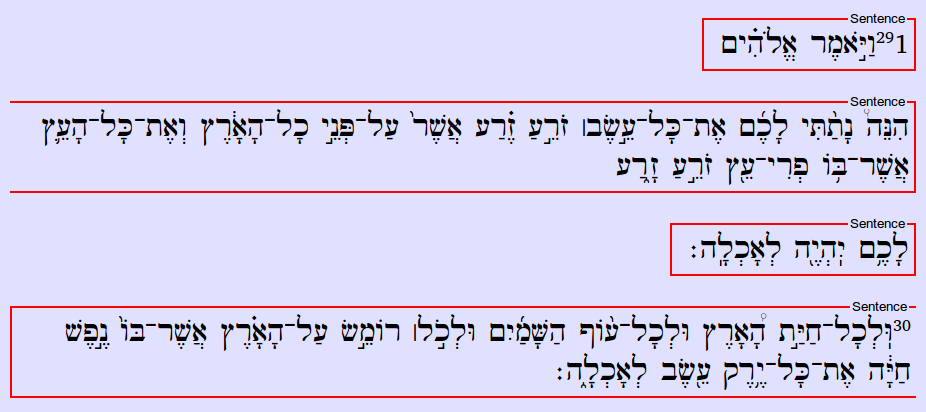
\includegraphics[width=0.9\textwidth]{gen1_29-30.png}
\end{center}

The sentence starting with the word \heb{הִנֵּה֩} consists of two parts. One sentence\_atom starts at
\heb{הִנֵּה֩} and ends at \heb{זָ֑רַע}, another sentence\_atom starts at \heb{וּֽלְכָל־חַיַּ֣ת} and ends at
\heb{לְאָכְלָ֑ה}. Together, these two sentence\_atoms make up a single sentence. If a sentence is
contiguous, it contains a single sentence\_atom.

As illustrated above, Bible OL displays noncontiguous sentences using boxes where one of the sides is
missing.

Sentence objects consist of \emph{clause}\index{clause} objects, which -- like sentences -- are comprised of
\emph{clause\_atom}\index{clause\_atom} objects.

Clause objects consists of \emph{phrase}\index{phrase} objects, which are comprised of
\emph{phrase\_atom}\index{phrase\_atom} objects.

Phrase objects may contain \emph{subphrase}\index{subphrase} objects. Note the word ``may''; not all words belong to
a subphrase. Subphrase objects are always built from contiguous monads. Subphrases may contain other
subphrases; for example, in \bibleref{Genesis}{1}{16} the words \heb{וַיַּ֣עַשׂ אֱלֹהִ֔ים
    אֶת־שְׁנֵ֥י הַמְּאֹרֹ֖ת הַגְּדֹלִ֑ים} contain three subphrases:

\begin{itemize}
\item \heb{שְׁנֵ֥י}
\item \heb{הַמְּאֹרֹ֖ת הַגְּדֹלִ֑ים}
\item \heb{הַגְּדֹלִ֑ים}
\end{itemize}


Note how the third subphrase is part of the second subphrase.

\subsubsection{Editorial Object Types}

The object types \emph{book, chapter, verse,} and \emph{half\_verse} describe the editorial composition of the
text.

The objects \emph{book,}\index{book} \emph{chapter,}\index{chapter} and \emph{verse}\index{verse}
are self-explanatory. The \emph{half\_verse}\index{half\_verse} objects identify a subdivsion of
verses into two halves, labelled A and B. For example, in \bibleref{Genesis}{1}{1}, the two
half\_verse objects correspond in English to:

\begin{itemize}
\item[A:] In the beginning God created
\item[B:] the heavens and the earth.
\end{itemize}


\subsection{What Is a Word?}\label{sec-contin}\index{word}

In most western languages, a space\index{space (between words)} is inserted between two words. In
Hebrew, some words are strung together as one. For example, the text ``\heb{וַֽיְהִי־אֹֽור׃}'' (``and there was
light'') in \bibleref{Genesis}{1}{3} consists of the three words \heb{וַֽ} (``and''), \heb{יְהִי}
(``there was''), and \heb{אֹֽור} (``light'').

In ETCBC4 this problem is handled by associating an Emdros feature called
\emph{suffix}\index{suffix|hyperit} with each word. The suffix feature contains

\begin{itemize}
\item a space if a space should be inserted between this word and the next,
\item an empty string if this word should be strung together with the following word,
\item a \heb{־} (Unicode\index{Unicode} value 05BE) if a \emph{maqaf}\index{maqaf} (hyphen) should to be inserted
  between this word and the next,
\item punctuation characters, such as the a \heb{׃} (Unicode\index{Unicode} value 05C3), which is
  the verse termination character, \emph{sof pasuq}.
\end{itemize}

So for the text ``\heb{וַֽיְהִי־אֹֽור׃}'', mentioned above, we have these features for the three words:

\begin{my-tabu}{cc}{ \headii{Text}{Suffix} }
  \heb{וַֽ} & Empty string\\
  \heb{יְהִי} & \emph{Maqaf}\\
  \heb{אֹֽור} & \emph{Sof pasuq} followed by space\\
\end{my-tabu}

The actual name of the \emph{suffix} feature varies from one Emdros database to another. (See
``suffixFeature'' on page \pageref{suffixFeature}.)

Note: The \emph{suffix} feature mentioned here must not be confused with the grammatical suffix that can be added
to a Hebrew word. For example, in \bibleref{Genesis}{1}{12} the word \heb{מִינֵ֔הוּ}, which derives from
the lexeme \heb{מִין}, has a grammatical suffix indicating \emph{3rd person, masculine, singular}.

%%%%%%%%%%%%%%%%%%%% Nestle1904 %%%%%%%%%%%%%%%%%%%%
\section{Nestle1904}\index{nestle1904|hyperit}

This section describes a number of features of the nestle1904 Greek database. A more detailed
description can be found in Appendix \ref{app-nestle}.

\subsection{Object Types}\index{Emdros!object}

The nestle1904 database contains these object types:

\begin{itemize}
\item word\index{word}
\item sentence\index{sentence}
\item clause1\index{clause1}
\item clause2\index{clause2}
\item book\index{book}
\item chapter\index{chapter}
\item verse\index{verse}
\end{itemize}

\subsubsection{Syntactic Object Types}

The object types \emph{word, sentence, clause1,} and \emph{clause2} describe the syntactic
composition of the text.

The basic object type is the \emph{word.}\index{word} Each \emph{word} corresponds to a single
monad.\index{monad} In contrast to the Hebrew database, the Greek database has no concept of a
\emph{suffix}\index{suffix} feature (see Section \ref{sec-contin}).

The top-level syntactic element is the \emph{sentence.}\index{sentence} A sentence is a set of
contiguous monads.

Sentence objects contain \emph{clause1}\index{clause1} objects. A \emph{clause1} object may be built from sets of
noncontiguous monads. Consider, for example, \bibleref{Luke}{2}{17}:

\begin{center}
  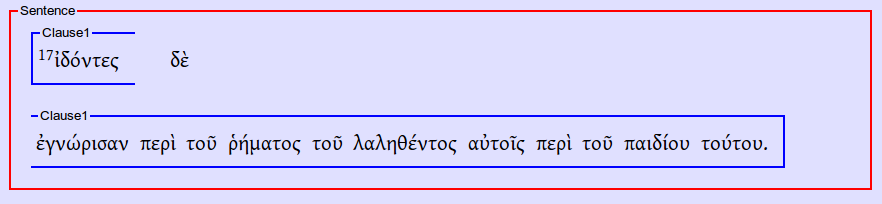
\includegraphics[width=0.9\textwidth]{luke2_17.png}
\end{center}

This sentence contains a single \emph{clause1} object, but the word \emph{δὲ} is not considered part
of that object. As illustrated above, Bible OL displays noncontiguous \emph{clause1} objects using
boxes where one of the sides is missing.

\emph{Clause1} objects may contain \emph{clause2}\index{clause2} objects, which -- like
\emph{clause1} objects -- may be noncontiguous.

\subsubsection{Editorial Object Types}

The object types \emph{book, chapter,} and \emph{verse} describe the editorial composition of the
text.\index{book}\index{chapter}\index{verse}

%%%%%%%%%%%%%%%%%%%% A Note on Greek Accents in Unicode %%%%%%%%%%%%%%%%%%%%
\section{A Note on Greek Accents in Unicode}\index{Unicode}\index{accent!Greek}\index{Greek accent|see {accent, Greek}}

Classical Greek used polytonic accents%
\index{accent!polytonic}\index{polytonic accent|see {accent, polytonic}}
over vowels. For example, the letter alpha could have these polytonic accents:

\begin{my-tabu}{cll}{ \headiii{Character}{Greek accent name}{English accent name} }
    ά & Oxia\index{oxia} (οξεία) & Acute\index{accent!acute}\index{acute accent|see {accent, acute}}\\
    ὰ & Varia\index{varia} (βαρεία) & Grave\index{accent!grave}\index{grave accent|see {accent, grave}}\\
    ᾶ & Perispomeni\index{perispomeni} (περισπωμένη) & Circumflex\index{accent!circumflex}\index{circumflex accent|see {accent, circumflex}}\\
\end{my-tabu}

Modern Greek is not a polytonic language, and in 1982 the polytonic accents were replaced by a
single, monotonic accent\index{accent!monotonic}\index{monotonic accent|see {accent, monotonic}}:
the \emph{tonos}\index{tonos} (τόνος). In the early years of the monotonic system, particularly when
reformers wished to differentiate their system from the polytonic, the tonos on letters was a novel
sign: typically a dot or wedge: α\hspace{-0.5mm}̍\hspace{0.5mm}. However, the Greek government
decreed in 1986 that the tonos shall be the acute. So you must now write ά instead of
α\hspace{-0.5mm}̍\hspace{0.5mm}.\footnote{Source:
  \url{http://www.opoudjis.net/unicode/unicode_gkbkgd.html}, accessed 2 September 2019.}

This confusion has had an impact on the representation of the oxia and tonos accents in Unicode.
Because of the decision from 1982, Unicode\index{Unicode} distinguishes between the oxia
and the tonos; but because of the decision from 1986, a change was made in Unicode
version 3.0 stating that the character ά should be encoded with the Unicode value for GREEK SMALL
LETTER ALPHA WITH TONOS, even when writing ancient Greek.

The affected Unicode characters are:

\begin{center}
  \begin{tabu}{@{}ccc@{}}
    \toprule
    & \multicolumn{2}{c}{\textbf{Unicode\index{Unicode} value with}}\\
    \cmidrule{2-3}
    \textbf{Character} & \textbf{tonos} & \textbf{oxia}\\
    \midrule
    ά & 03AC & 1F71\\
    έ & 03AD & 1F73\\
    ή & 03AE & 1F75\\
    ί & 03AF & 1F77\\
    ό & 03CC & 1F79\\
    ύ & 03CD & 1F7B\\
    ώ & 03CE & 1F7D\\
    ΐ & 0390 & 1FD3\\
    ΰ & 03B0 & 1FE3\\
    \bottomrule
  \end{tabu}
\end{center}

So nowadays the correct way to encode the character ά is to use the value 03AC, regardless of
whether the accent is an oxia or a tonos.

But here's the catch: \emph{The nestle1904\index{nestle1904} database uses the oxia encodings, not
  the recommended tonos encodings.} (The reason is probably a desire to emphasize that polytonic
accents are used.)

This necessitates a conversion between tonos\index{tonos} encoding and oxia\index{oxia} encoding in
a few places in Bible OL.




%%%%%%%%%%%%%%%%%%%%%%%%%%%%%%%%%%%%%%%%%%%%%%%%%%%%%%%%%%%%%%%%%%%%
%%%%%%%%%%%%%%%%%%%% Database Description Files %%%%%%%%%%%%%%%%%%%%
\chapter{Database Description Files}\index{Database Description File}\index{Description File|see {Database Description File}}

\textbf{Read this chapter if you are going to work with code that accesses the Emdros databases on
  the server or displays text and exercises in the client.}
\plainbreak{3}


Each database is associated with a number of files that describe details about the database. They
are collectively known as the \emph{Database Description Files}. This chapter describes these files
in detail.

In the Bible OL source tree, the Database Description Files are found in the directory \texttt{db}.

The names of Database Description Files consist of a so-called \emph{primary name}%
\index{primary name|hyperit}
and a suffix. For example, one Database Specification File is
\texttt{ETCBC4-translit.db.json}. Here the primary name is ``\texttt{ETCBC4-translit}'' and the
suffix is ``\texttt{.db.json}''.

The following table lists the suffixes of various Database Description Files:

\begin{my-tabu}{>{\ttfamily}llc}{ \headiii{\textrm{Suffix}}{Type}{Described in Section} }
.db.json &
Database Specification File\index{Database Specification File}\index{Specification File|see {Database Specification File}} &
\ref{sec-dsf}\\

.typeinfo.json &
Database Type Information File\index{Database Type Information File}\index{Type Information File|see {Database Type Information File}} &
\ref{sec-tif}\\

.glosslang.json &
Lexicon Information File\index{Lexicon Information File}\index{glosslang file|see {Lexicon Information File}} &
\ref{sec-lif}\\

.bookorder &
Database Book Order File\index{Database Book Order File}\index{Book Order File|see {Database Book Order File}} &
\ref{sec-bookorder}\\

\end{my-tabu}

In the following sections the string ``PRIM'' is used to denote the primary name of a file.

\pfbreak

Most of the files are JSON\index{JSON} files. A JSON file contains key/value pairs%
\index{key value pairs@key/value pairs},
where the value can be a string, a number, a Boolean value, an array of values, or another
collection of key/value pairs.

A JSON file can either be ``ugly''%
\index{JSON!ugly file|hyperit}\index{ugly JSON file|see {JSON, ugly file}}
or ``pretty''%
\index{JSON!pretty file|hyperit}\index{pretty JSON file|see {JSON, pretty file}}.
This is an example of an ugly JSON file:

\begin{lstlisting}
{"alpha":8,"beta":{"gamma":true,"delta":["ten","eleven"]}}
\end{lstlisting}

This is the same data in pretty format:

\begin{lstlisting}
{
    "alpha": 8,
    "beta": {
        "gamma": true,
        "delta": [
            "ten",
            "eleven"
        ]
    }
}
\end{lstlisting}

Both of these listings describe the same object. The object contains two key/value pairs:

\begin{itemize}
\item ``alpha'' with the numerical value 8.
\item ``beta'' with a value that is a collection of key/value pairs.
\end{itemize}

The key ``beta'' has a value that contains two key/value pairs:

\begin{itemize}
\item ``gamma'' with the Boolean value \emph{true}.
\item ``delta'' with a value that is an array containing the two strings ``ten'' and ``eleven''.
\end{itemize}


Bible OL works equally well with ugly and pretty JSON files, but the ugly format is normally
preferred because it takes up less space (and makes reverse engineering slightly more difficult for
the uninitiated). The pretty format is, of course, easier for humans to understand is therefore useful
while debugging the system.

The script \emph{json\_pretty\_print.php}\index{json\_pretty\_print.php} can be used to convert
between the ugly\index{JSON!ugly file} and the pretty\index{JSON!pretty file} format. If the file
``xxx.json'' contains JSON data (either ugly or pretty), the command

\begin{lstlisting}[language=bash]
php json_pretty_print.php -p xxx.json
\end{lstlisting}

\noindent
will write the data in pretty format to standard output; and the command

\begin{lstlisting}[language=bash]
php json_pretty_print.php -u xxx.json
\end{lstlisting}

\noindent
will write the data in ugly format to standard output.

The directory \texttt{db} contains JSON files in both the ugly and the pretty format. For example,
the file \texttt{ETCBC4.db.json} is the ugly version of \texttt{ETCBC4.db.pretty.json}. The
developer should only modify the \texttt{.pretty.json} files and then run the
\emph{Makefile} in the top source directory, which will generate the corresponding ugly JSON files.




%%%%%%%%%%%%%%%%%%%% Database Specification File: PRIM.db.json %%%%%%%%%%%%%%%%%%%%
\section{Database Specification File: PRIM.db.json}\label{sec-dsf}\index{Database Specification File|hyperit}

\textbf{On the server} the \emph{Database Specification File} has a name that ends in \texttt{.db.json}. For Bible OL,
this is the main point of access to the Emdros databases. When Bible OL needs to list the available
databases, it searches for files with names that end in \texttt{.db.json}.

\textbf{On the client} the contents of the Database Specification File is available in a variable
called \emph{configuration.}%
\index{configuration JavaScript variable@\emph{configuration} JavaScript variable|hyperit}
Its structure is described in TypeScript as the \emph{Configuration}%
\index{Configuration TypeScript interface@\emph{Configuration} TypeScript interface}
interface in the file \texttt{ts/configuration.ts}.

The Database Specification File describes how the individual parts of an Emdros database are used by Bible
OL. It describes what features are available for exercises and what grammatical features the user
can choose to display.

Multiple Database Specification Files can refer to the same Emdros database. For example,
\texttt{ETCBC4.db.json} and \texttt{ETCBC4-translit.db.json} both reference the ETCBC4 Emdros
database, but the former displays text using the native alphabet\index{alphabet!native}, whereas the
latter displays text using the transliterated alphabet\index{alphabet!transliterated}.

The Database Specification File is a JSON file containing the following key/value pairs:

\begin{my-longtabu}{lX}{ \headii{Key}{Value} }
  version & A number which identifies the layout used by this file. This number is currently ignored.\\

  databaseName\label{databasename} & The name of the Emdros database file. Currently, this is either
  ``ETCBC4'' or ``nestle1904''. This is also the primary name\index{primary name} of the Database
  Type Information File\index{Database Type Information File} (see Section \ref{sec-tif}) and
  Database Book Order File\index{Database Book Order File} (see Section \ref{sec-bookorder}).\\

  propertiesName\label{propname} & The name of the Grammar Localization
    Struture\index{Grammar Localization Structure} (see Section \ref{sec-gram-loc-struct}).\\

  databaseVersion & A string containing the version number of the database. This number is only used
  for display purposes. Whenever an Emdros database is changed, this number should also be changed.\\

  granularity & The name of the Emdros object type defining the amount of text to display in an exercise.
  Typically, this name is ``sentence''.\index{sentence}\\

  surfaceFeature & The actual name of the \emph{visual} feature%
  \index{visual feature@``visual'' feature}
  (see Section \ref{sec-visual}). For ETCBC4 using the native alphabet this value is
  ``g\_word\_utf8'', for ETCBC4 using the transliterated alphabet the value is
  ``g\_word\_translit'', for nestle1904 the value is ``surface''.\\

  objHasSurface & The name of the Emdros object type that contains the \emph{surfaceFeature.}
  (Typically, ``word''.)\\

  suffixFeature\label{suffixFeature} & The actual name of the \emph{suffix} feature%
  \index{suffix} (see Section \ref{sec-contin}). For ETCBC4 using the native alphabet this value is
  ``g\_suffix\_utf8'', for ETCBC4 using the transliterated alphabet the value is
  ``g\_suffix\_translit'', for nestle1904 the value is \emph{null}. \\

  charSet & The name of the character set for the text. For ETCBC4
  using the native alphabet this value is ``hebrew'', for ETCBC4
  using the transliterated alphabet the value is ``transliterated\_hebrew'', for nestle1904 the value is ``greek''.\\

  objectSettings\index{objectSettings} & A collection of key/value pairs containing information about how Bible OL should
  treat Emdros object type. This is detailed in Section \ref{sec-objectsettings}.\\

  universeHierarchy & An array containing information about how the text references are structured.
  For the Bible, this hierarchy is book/chapter/verse.%
  \index{passages!hierarchy}
  A typical value is\label{universe-hierarchy}

  {\ttfamily
    \begin{tabular}{lll}
      \multicolumn{3}{l}{"universeHierarchy": [}\\
         & \{ &                      \\
         &    &  "type": "book",     \\
         &    &  "feat": "book"      \\
         & \},&                      \\
         & \{ &                      \\
         &    &  "type": "chapter",  \\
         &    &  "feat": "chapter"   \\
         & \},&                      \\
         & \{ &                      \\
         &    &  "type": "verse",    \\
         &    &  "feat": "verse"     \\
         & \} &                      \\
      ]  &    &                      \\
    \end{tabular}
  }

  This means that the top reference level is found in the \emph{book}\index{book} feature of Emdros
  objects of type \emph{book}, the second reference level is found in the
  \emph{chapter}\index{chapter} feature of Emdros objects of type \emph{chapter}, and the third
  reference level is found in the \emph{verse}\index{verse} feature of Emdros objects of type
  \emph{verse}.
  
  Note that in several locations, code in Bible OL is hard-coded to rely on the book/chapter/verse
  structure used in the Bible.\\

  picDb & The URL of the resource website\index{resource website} (see Section
  \ref{sec-resource-web}). This value may be \emph{null.}\\

  sentencegrammar & An array containing information about the grammar items available to the user.
  This is detailed in Section \ref{sentencegrammar}.\\

  subsetOf & If the Database Specification File describes a subset\index{subset} of a larger database,
  \emph{subsetOf} gives information about the subset. This is detailed in Section
  \ref{subsetof}. This value is always \emph{null} for the ETCBC4 and nestle1904
  databases.\\

\end{my-longtabu}


\subsection{The \emph{objectSettings} Key}\label{sec-objectsettings}\index{objectSettings|hyperit}

The \emph{objectSettings} key in the Database Specification File gives detailed information about
how the Emdros object types and their features should be treated by Bible OL. The
\emph{objectSettings} key has a value that is a collection of key/value pairs, where the keys are
Emdros object type. The corresponding values give information about how the Emdros object should be
treated.

Listing \ref{list-ossample} shows a subset of the \emph{objectSettings} for the ETCBC4 database.

\begin{lstlisting}[caption=A sample objectSettings value,label=list-ossample]
    "objectSettings": {
        "book": {
        },
        "chapter": {
        },
        "verse": {
        },
        "word": {
            "mayselect": true,
            "additionalfeatures": [...],
            "featuresetting": {...}
        },
        "subphrase": {
            "mayselect": true,
            "featuresetting": {...}
        }
    }
\end{lstlisting}

In this subset, the Emdros types \emph{book, chapter, verse, word,} and \emph{subphrase} are
mentioned. No special information about \emph{book, chapter,} and \emph{verse} is provided, which
means that these Emdros types cannot be made the subject of exercises. It is the presence of the key
\emph{mayselect}\index{mayselect} with the value \emph{true} that signals to Bible OL that the associated Emdros
object can be used when selecting quiz objects\index{quiz object (a.k.a. sentence unit)} for an exercise. So in the example in Listing
\ref{list-ossample}, the Emdros objects \emph{word} and \emph{subphrase} can be used for quiz object
selection.

When you are creating an exercise with the ETCBC4 database, the ``Sentences'' and ``Sentence Units''
tabs allow you to specify a sentence unit (a.k.a. quiz object\index{quiz object (a.k.a. sentence unit)}) type:

\begin{center}
  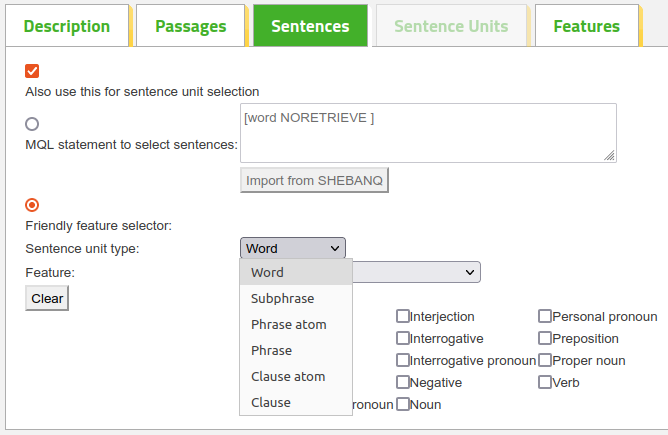
\includegraphics[width=0.9\textwidth]{senselect.png}
\end{center}

The values in the drop down box are the Emdros object that have \emph{mayselect}\index{mayselect} set to \emph{true}
in \emph{objectSettings.}\index{objectSettings} As shown in Listing \ref{list-ossample}, these objects have one or
two additional key/value pairs with the keys \emph{featuresetting} and, optionally,
\emph{additionalfeatures.}

The value of \emph{featuresetting} is another collection of key/value pairs, giving
details about the features of the object. This is detailed in Section \ref{sec-featuresetting}.

The \emph{additionalfeatures} key identifies an array of features that should always be retrieved
for this Emdros object, even though these features are not the subject of an exercise. They are used
for accessing the multiple choice\index{multiple-choice} database (see Chapter \ref{chap-multiple-choice}).

\subsection{The \emph{featuresetting} Key}\label{sec-featuresetting}\index{featuresetting}

The \emph{featuresetting} key under an Emdros object type gives detailed information about how the
features\index{Emdros!feature} of the Emdros object should be treated by Bible OL. Its value is a collection of key/value
pairs, where the keys are feature names. The corresponding values give
information about how the feature should be treated.

Listing \ref{list-fssample} shows a subset of the \emph{featuresetting} for the \emph{word} object
in the ETCBC4 database.

\begin{lstlisting}[escapechar=\#,caption=A sample featuresetting value,label=list-fssample]
    "featuresetting": {
        "lexeme_occurrences": {
            "ignoreShow": true,
            "ignoreRequest": true,
            "isRange": true
        },
        "english": {
            "ignoreSelect": true,
            "matchregexp": "\/^(.+[;,] +)?(\\(.*\\) *)?{0}( *\\(.*\\))?([,;].+)?$\/i",
        },
        "g_word_cons_utf8": {
            "hideWord": true,
            "foreignText": true
        },
        "g_word_nocant_utf8": {
            "alternateshowrequestDb": "ETCBC4_words.db",
            "alternateshowrequestSql": "SELECT DISTINCT word FROM texts,lextext,lexemes WHERE lex='%s' AND lexid=lexemes.id AND textid=texts.id",
            "hideWord": true,
            "foreignText": true
        },
        "vt": {
            "hideValues": [
                "weyq"
            ]
        }
    }
\end{lstlisting}

In this subset, the features \emph{lexeme\_occurrences, english, g\_word\_const\_utf8,
  g\_word\_nocant\_utf8,} and \emph{vt} are mentioned. The value associated with each of these keys is
another collection of key/value pairs. Many of the values are Boolean, and an absent key is
equivalent to a Boolean value of \emph{false}. Thus, the absence of a \emph{hideWord} key from
\emph{lexeme\_occurrences} has the same meaning as if \emph{hideWord} had been given the value
\emph{false.}

The following table lists the keys and values that can be associated with a feature of an Emdros
object:

\begin{my-longtabu}{X[0.3,l]X[0.7]}{ \headii{Key}{Value} }
  ignoreSelect & A value of \emph{true} means: Do not use this feature for object selection (see
  below).\\

  isDefault & This value must be \emph{true} for exactly one feature of an Emdros object. It
  indicates that this feature is the initially displayed feature in the ``Sentences'' tab when
  creating an exercise (see below).\\

  ignoreShow & A value of \emph{true} means that this feature cannot be displayed as part of an
  exercise. In other words, there is no ``Show'' button for this feature on the ``Features'' tab
  when creating an exercise.\\

  ignoreRequest & A value of \emph{true} means that this feature cannot be requested as part of an
  exercise. In other words, there is no ``Request'' button for this feature on the ``Features'' tab
  when creating an exercise.\\

  hideWord & If this value is \emph{true} and the feature is a request feature for an exercise, the
  corresponding words should be replaced by a number in
  the displayed text (see below).\\

  foreignText & A value of \emph{true} means that this feature is written using a non-Latin
  alphabet.\\

  transliteratedText & A value of \emph{true} means that this feature is written using the
  transliterated Hebrew alphabet.\\

  hideValues & Relevant only for enumeration%
  \index{Emdros!enumeration}\index{enumeration|see {Emdros, enumeration}}
  features. It is an array of enumeration values
  that never occur in a text and should therefore be omitted from the user interface.\\

  isRange & A value of \emph{true} means that this feature represents range of integer
  values.\\

  otherValues & An array of enumeration\index{Emdros!enumeration} feature values that should be lumped together as ``Other'' in
  the user interface. (This is not currently used by any Emdros databases in Bible OL.)\\

  matchregexp & A regular expression used to check if an answer provided by a learner matches the
  value of a feature. For example, the \emph{english} feature for the Hebrew word \heb{אֶרֶץ} has the value
  ``land; territory, country; the earth''. The regular expression in \emph{matchregexp} is designed
  to ensure that a learner's answer is accepted, regardless of whether the answer is ``land'',
  ``territory'', ``country'', or ``the earth''.\\

  alternateshowrequestDb & The name of a multiple choice\index{multiple-choice} database (see
  Chapter \ref{chap-multiple-choice}).\\

  alternateshowrequestSql & An SQL statement used to access the multiple choice%
  \index{multiple-choice}
  database (see Chapter \ref{chap-multiple-choice}).\\

  indirdb, sql\_command, sql\_command\_variant, sqlargs, multiple & These keys are used for pseudofeatures. See Section
  \ref{sec-pseudofeature}. \\
  
\end{my-longtabu}


The keys \emph{ignoreSelect} and \emph{isDefault} control the contents of the feature selection
menu when creating an exercise:

\begin{center}
  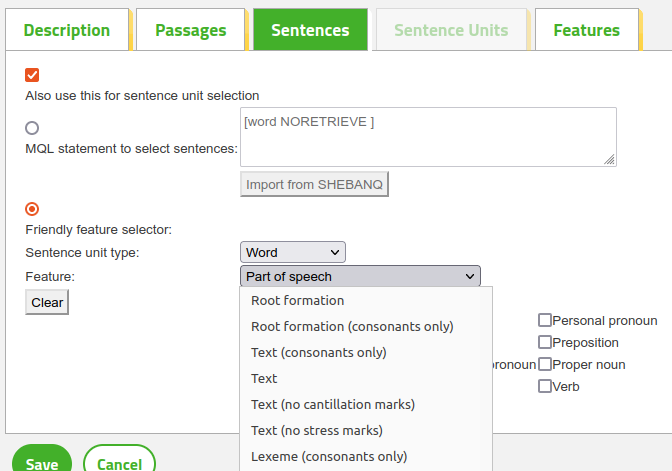
\includegraphics[width=0.9\textwidth]{featselect.png}
\end{center}

If \emph{ignoreSelect} is set for a feature, then that feature is not shown in the selection menu.
The feature with \emph{isDefault} set is the selected feature when the dialog is first loaded.

If \emph{hideWord} is \emph{true} and the feature is used as a request feature%
\index{request feature}
in an exercise, the corresponding word is replaced by a number in the text. For example,
in the following exercise the feature \emph{text\_nocant\_utf8} (that is, ``Text (no cantillation
marks)'') is used as a request feature. Consequently the corresponding words in the text are
replaced by the numbers (1), (2), and (3) lest the words in the text give the answer to the
questions:


\begin{center}
  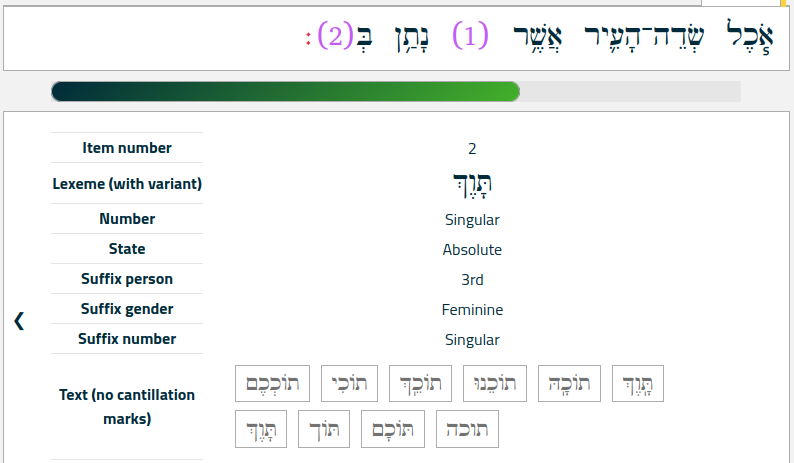
\includegraphics[width=0.9\textwidth]{numbers.png}
\end{center}

\subsubsection{Pseudofeatures}\label{sec-pseudofeature}\index{pseudofeature|hyperit}

The features listed in the \emph{featuresetting} information are normally genuine feature of Emdros
objects. However, a few of them may be \emph{pseudofeatures}. A pseudofeature is logically
associated with an Emdros object just as ordinary features are, but the values of pseudofeatures are
retrieved from other data sources.

As an example of a pseudofeature, consider Listing \ref{list-ps-syntax}.

\begin{lstlisting}[escapechar=\#,caption=Featuresetting syntax for a pseudofeature,label=list-ps-syntax]
    "glossurl": {
        "ignoreSelect": true,
        "indirdb": "mysql",
        "sql_command": "SELECT url, icon FROM {PRE}heb_urls WHERE lex='%s' AND language='%s'",
        "sqlargs": [
            "lex",
            "language"
        ],
        "multiple": true
    }
\end{lstlisting}

A pseudofeature uses the keys \emph{indirdb, sql\_command, sql\_command\_variant, sqlargs,} and \emph{multiple.}

\begin{itemize}
\item \emph{indirdb} gives the name of a database in which the pseudofeature can be found. The value
  is either the name of an SQLite3\index{SQLite3} database, or the string ``mysql'' if the
  pseudofeature is found in the user database\index{user database} (see Section
  \ref{chap-user-database}).
\item \emph{sql\_command} is the SQL command required to retrieve the value of the feature. A
  typical example is given in the listing above. The system will replace the string \texttt{\{PRE\}}
  with the correct database table prefix. Each occurrence of the string \texttt{\%s} will be
  replaced by the value of a feature named in \emph{sqlargs}. Alternatively the strings
  \texttt{\%1\$s}, \texttt{\%2\$s}, etc. can be used to specify a specific entry in \emph{sqlargs}.
\item \emph{sql\_command\_variant} (not shown in Listing \ref{list-ps-syntax}) is the SQL command
  required to retrieve a variant value (see Section \ref{sec-variants}) of the feature. Its syntax is
  similar to that of \emph{sql\_command}.
\item \emph{sqlargs} is an array of features whose values are to be used in place of the
  \texttt{\%s} strings in \emph{sql\_command} and \emph{sql\_command\_variant}.
\item \emph{multiple} is true if the database may contain more than one record for a given pseudofeature.
\end{itemize}

Taking the pseudofeature \emph{glossurl} from Listing \ref{list-ps-syntax} as an example, we see that
the feature is found in the user database because \emph{indirdb} has the value ``mysql''.

If we assume that the database table prefix\footnote{The database table prefix can be set in the
  file \texttt{myapp/config/database.php} (See Section \ref{sec-database-php}).} is ``bol\_'', and
if the \emph{lex} and \emph{language} features have the values ``B.@R@>'' and ``Hebrew'', respectively,
the value of the pseudofeature is found by executing the SQL query

\begin{lstlisting}[language=SQL]
SELECT url, icon FROM bol_heb_urls WHERE lex='B.@R@>' AND language='Hebrew'
\end{lstlisting}

The SQL query is allowed to return multiple values because \emph{multiple} is \emph{true.}


\subsubsection{The ``gloss'' Feature}\label{sec-gloss-feature}\index{gloss feature@``gloss'' Feature}

The feature named ``gloss'' is treated specially. Bible OL automatically replaces it with a number
of features each representing a taget language for a lexicon. The ``gloss'' feature must have
an \emph{sql\_command} setting that contains the string ``LANG''. This string will be replaced by
the language code for the target language. If an \emph{sql\_command\_variant} setting is present, it must
contain the strings ``LANG'' and ``VARIANT'', which will be replaced by the language code and the
variant name, respectively. For example, the ``gloss'' feature specification may look
like this:

\begin{lstlisting}[escapechar=\#]
    "gloss": {
        ...
        "sql_command": "SELECT gloss FROM {PRE}lexicon_%1$s h JOIN {PRE}lexicon_%1$s_LANG lang ON lang.lex_id=h.id WHERE lex='%2$s' AND vs='%3$s'",
        "sqlargs": [
            "language",
            "lex",
            "vs"
        ],
        ...
    }
\end{lstlisting}

Bible OL may replace this with these specifications:

\begin{lstlisting}[escapechar=\#]
    "english": {
        ...
        "sql_command": "SELECT gloss FROM {PRE}lexicon_%1$s h JOIN {PRE}lexicon_%1$s_en lang ON lang.lex_id=h.id WHERE lex='%2$s' AND vs='%3$s'",
        "sqlargs": [
            "language",
            "lex",
            "vs"
        ],
        ...
    }
    "german": {
        ...
        "sql_command": "SELECT gloss FROM {PRE}lexicon_%1$s h JOIN {PRE}lexicon_%1$s_de lang ON lang.lex_id=h.id WHERE lex='%2$s' AND vs='%3$s'",
        "sqlargs": [
            "language",
            "lex",
            "vs"
        ],
        ...
    }
\end{lstlisting}



\subsection{The \emph{sentencegrammar} Key}\label{sentencegrammar}\index{sentencegrammar}

The \emph{sentencegrammar} key in the Database Specification File gives detailed information about
the grammar items available to the user. Its value is an array, in which each entry
corresponds to an Emdros object type.

Bible OL uses the information in \emph{sentencegrammar} in two locations. One is the grammar
selection box\index{grammar selection box} in the left part of the screen, the other is in the
grammar information box\index{grammar information box} in the right part of the screen.

The grammar selection box\index{grammar selection box} may look like this:

\begin{center}
  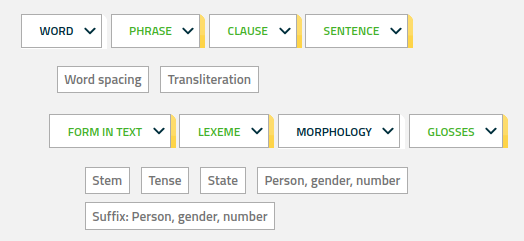
\includegraphics[width=0.3\textwidth]{grammarselect.png}\label{grammarselect}
\end{center}

In the above illustration, each of the four main menus, \emph{Word, Phrase, Clause,} and
\emph{Sentence,} of the grammar selection box corresponds to an entry at the top level of
\emph{sentencegrammar}.

The grammar information box\index{grammar information box} may look like this:

\begin{center}
  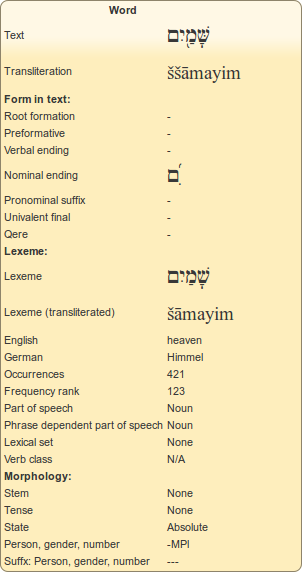
\includegraphics[width=0.5\textwidth]{grammarinfo.png}
\end{center}

In this illustration, the \emph{sentencegrammar} for the \emph{word} object
has been used to determine what information to retrieve.

Listing \ref{list-sgsample} shows the \emph{sentencegrammar} for the ETCBC4 database (taken from the
file \texttt{db/ETCBC4.db.json}).

\begin{lstlisting}[caption=Condensed sentencegrammar value,label=list-sgsample]
    "sentencegrammar": [
        {
            "mytype": "SentenceGrammar",
            "objType": "word",
            "items": [...]
        },
        {
            "mytype": "SentenceGrammar",
            "objType": "phrase",
            "items": [...]
        },
        {
            "mytype": "SentenceGrammar",
            "objType": "clause",
            "items": [...]
        },
        {
            "mytype": "SentenceGrammar",
            "objType": "sentence"
        }
    ]
\end{lstlisting}

As this example shows, \emph{sentencegrammar} is an array whose elements have
three key/value pairs:

\begin{itemize}
\item \emph{mytype} with a value that is always ``SentenceGrammar''.
\item \emph{objType} with a value that identifies an Emdros object.
\item \emph{items} (optional), which is an array of \emph{GrammarFeature,
  GrammarMetaFeature,} \emph{GrammarGroup,} or \emph{GrammarGroupGlosses} specifications, as detailed below.
\end{itemize}

If you compare the listing of \emph{sentencegrammar} above, with the grammar selection box shown on
page \pageref{grammarselect}, you will notice that each element in the \emph{sentencegrammar}
corresponds to a top level box in the illustration.

For each Emdros object (that is, for each element in the \emph{sentencegrammar} array) the value of
\emph{items} is an array that specified the features that can be displayed for the particular Emdros
object. Each entry in the \emph{items} array can have one of four forms: \emph{GrammarFeature,
  GrammarMetaFeature,} \emph{GrammarGroup}, or \emph{GrammarGroupGlosses}, as specified in their \emph{mytype} value.

Listing \ref{list-itemssample} shows a typical \emph{items} array.

\begin{lstlisting}[caption=A sample items value,label=list-itemssample]
    "items": [
        {
            "mytype": "GrammarFeature",
            "name": "g_word_translit"
        },
        {
            "mytype": "GrammarGroup",
            "name": "form_in_text",
            "items": [...]
        },
        {
            "mytype": "GrammarMetaFeature",
            "name": "pgn",
            "items": [...]
        }
    ]
\end{lstlisting}

In this example, the \emph{items} array has three elements, one with \emph{mytype=GrammarFeature},
one with \emph{mytype=GrammarGroup}, and one with \emph{mytype=GrammarMetaFeature.}

\subsection{GrammarFeature}\label{sec-grammarfeature}\index{GrammarFeature|hyperit}

A \emph{sentencegrammar} item with \emph{mytype=GrammarFeature} describes a single Emdros
feature. The format is given in Listing \ref{list-gf-syntax}.

\begin{lstlisting}[caption=GrammarFeature syntax,label=list-gf-syntax]
    {
        "mytype": "GrammarFeature",
        "name": %\textrm{\emph{an Emdros feature name}}%
    }
\end{lstlisting}

The \emph{name} value may simply be the name of a feature of the current Emdros object type, or it
may be a string in the form ``objectType:featureName'', if the feature belongs to another object
type. Alternatively, it may have the form ``objectType:featureName\texttt{\_TYPE\_}featureType'' if
a type other than the standard feature type is required. Currently, this is only used with the
ETCBC4 database, where the GrammarFeature name ``\texttt{clause\_atom:code\_TYPE\_text}'' is used to
denote a \emph{text} interpretation of the \emph{code} feature of the \emph{clause\_atom} object
type; the \emph{code} feature normally has type \emph{integer} rather than \emph{text.}

\Needspace*{5cm}%
In the grammar selection box\index{grammar selection box}, a GrammarFeature is displayed thus:

\begin{center}
  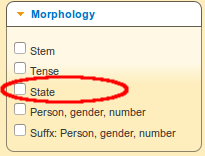
\includegraphics[width=0.3\textwidth]{state1.png}
\end{center}

\Needspace*{5cm}%
In the grammar information box\index{grammar information box}, a GrammarFeature is displayed thus:

\begin{center}
  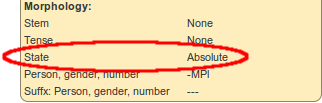
\includegraphics[width=0.5\textwidth]{state2.png}
\end{center}


\subsection{GrammarMetaFeature}\label{sec-grammarmetafeature}\index{GrammarMetaFeature|hyperit}

A \emph{sentencegrammar} item with \emph{mytype=GrammarMetaFeature} describes a combined value of a
number of Emdros features. Its format is given in Listing \ref{list-gmf-syntax}.

\begin{lstlisting}[caption=GrammarMetaFeature syntax,label=list-gmf-syntax]
    {
        "mytype": "GrammarMetaFeature",
        "name": %\textrm{\emph{the name of the GrammarMetaFeature}}%,
        "items": [
            {
                "mytype": "GrammarSubFeature",
                "name": %\textrm{\emph{an Emdros feature name}}%
            },
            {
                "mytype": "GrammarSubFeature",
            },
            ... %\textrm{\emph{Additional GrammarSubFeatures}}%
        ]
    }
\end{lstlisting}

In the \emph{items} array the Emdros features that make up the GrammarMetaFeature are listed with a
\emph{mytype} value of ``GrammarSubFeature''.\index{GrammarSubFeature|hyperit}

As an example, Bible OL combines the person, gender, and number of a word to a single item, such as
``2FSg'' (which means 2nd person, feminine, singular). This is specified as indicated in Listing
\ref{list-gmf-sample}.

\begin{lstlisting}[caption={A GrammarMetaFeature combining person, gender, and number},label=list-gmf-sample]
    {
        "mytype": "GrammarMetaFeature",
        "name": "pgn",
        "items": [
            {
                "mytype": "GrammarSubFeature",
                "name": "ps"
            },
            {
                "mytype": "GrammarSubFeature",
                "name": "gn"
            },
            {
                "mytype": "GrammarSubFeature",
                "name": "nu"
            }
        ]
    },
\end{lstlisting}

The \emph{ps, gn,} and \emph{nu} features represent the person, gender, and number of a word,
respectively.


\Needspace*{5cm}%
In the grammar selection box\index{grammar selection box}, a GrammarMetaFeature is displayed thus:

\begin{center}
  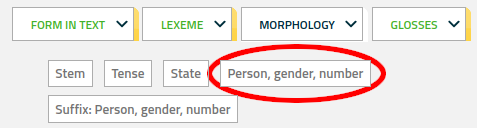
\includegraphics[width=0.3\textwidth]{pgn1.png}
\end{center}

\Needspace*{5cm}%
In the grammar information box\index{grammar information box}, a GrammarMetaFeature is displayed thus:

\begin{center}
  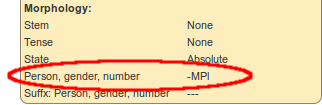
\includegraphics[width=0.5\textwidth]{pgn2.png}
\end{center}


\subsection{GrammarGroup}\label{sec-grammargroup}\index{GrammarGroup|hyperit}

A \emph{sentencegrammar} item with \emph{mytype=GrammarGroup} groups GrammarFeatures and
GrammarMetaFeatures into logical units, such as ``Features that describe the lexeme'' or ``Features
that describe the morphology''. Its format is given in Listing \ref{list-gg-syntax}.

\begin{lstlisting}[caption=GrammarGroup syntax,label=list-gg-syntax]
    {
        "mytype": "GrammarGroup",
        "name": %\textrm{\emph{the name of the GrammarGroup}}%,
        "items": [...]
    }
\end{lstlisting}

The \emph{items} array here contains a collection of GrammarFeatures and GrammarMetaFeatures in the
format described above.

\Needspace*{5cm}%
In the grammar selection box\index{grammar selection box}, a GrammarGroup (called ``Morphology'' in
this case) is displayed thus:

\begin{center}
\begin{tabular}{rcl}
  \vspace{0pt}\parbox{0.3\textwidth}{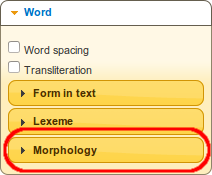
\includegraphics[width=0.3\textwidth]{morph1a.png}} %\vspace ensures center alignment
 & or &
  \vspace{0pt}\parbox{0.3\textwidth}{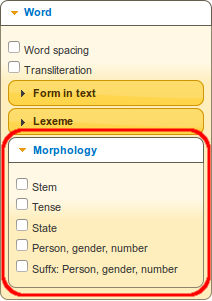
\includegraphics[width=0.3\textwidth]{morph1b.png}}
\end{tabular}
\end{center}

\Needspace*{5cm}%
In the grammar information box\index{grammar information box}, a GrammarGroup is displayed thus:

\begin{center}
  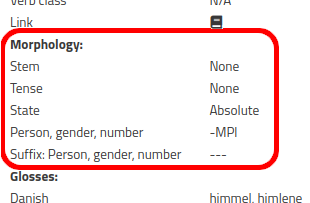
\includegraphics[width=0.5\textwidth]{morph2.png}
\end{center}


\subsection{GrammarGroupGlosses}\label{sec-grammargroupglosses}\index{GrammarGroupGlosses|hyperit}
 
A \emph{sentencegrammar} item with \emph{mytype=GrammarGroupGlosses} is a placeholder for
information about glosses that translate the source language of the Emdros database (such as Hebrew
or Greek) into a target language (such as English or German). The GrammarGroupGlosses entry must
always look as shown in Listing \ref{list-ggg-syntax}.
 
\begin{lstlisting}[caption=GrammarGroupGlosses syntax,label=list-ggg-syntax]
    {
        "mytype": "GrammarGroupGlosses",
        "name": "glosses",
        "items": []
    }
\end{lstlisting}
 
Bible OL will automatically replace this specification with a GrammarGroup specification that
contains all the available translations as separate GrammarFeatures. For example, Bible OL may
replace the GrammarGroupGlosses specification with this:
 
\begin{lstlisting}
    {
        "mytype":"GrammarGroup",
        "name":"glosses",
        "items": [
            {
                "mytype":"GrammarFeature",
                "name":"english"
            },
            {
                "mytype":"GrammarFeature",
                "name":"german"
            }
        ]
    }
\end{lstlisting}


\subsection{The \emph{subsetOf} Key}\label{subsetof}\index{subset|hyperit}

The \emph{subsetOf} value is present for historical reasons. With the current ETCBC4 and nestle1904
databases it is not required; however, the previously used WIVU\index{WIVU} database, was available in two
versions: the entire Old Testament and a subset containing about 20 per cent of the text.

The \emph{subsetOf} key specifies the relationship between the subset and the superset. It is used
to enable exercises that have been created for the subset to be used with the superset.

The format of \emph{subsetOf} is illustrated by this example taken from the subset Database
Specification File:

\begin{lstlisting}
    "subsetOf": {
        "name": "WIVU",
        "properties": "WIVU",
        "provides": [
            "Genesis",
            "Exodus:1",
            "Exodus:2",
            "Exodus:3",
            ... %\textrm{\scriptsize(Additional Bible references omitted)}%
        ]
    }
\end{lstlisting}

Here, \emph{name} is the name of the Emdros database file for the superset, and \emph{properties} is
the name of the Grammar Localization Struture\index{Grammar Localization Structure} (see
Section \ref{sec-gram-loc-struct}) for the superset.

The \emph{provides} array identifies the books and chapters provided by the subset. In this example,
the subset includes the entire book of Genesis and the first three chapters of Exodus.

If \emph{subsetOf} has the value \emph{null}, the current database is not a subset of any other
database.



%%%%%%%%%%%%%%%%%%%% Database Description Files for Old Databases %%%%%%%%%%%%%%%%%%%%
\section{Database Description Files for Old Databases}\label{sec-old-db}

Currently, Bible OL uses two databases, the Hebrew \emph{ETCBC4} database and the Greek
\emph{nestle1904} database. Previous versions of Bible OL used the Hebrew \emph{WIVU}\index{WIVU}
database (and various variants of it) and the Greek \emph{tisch}\index{tisch}\footnote{Short for
  \emph{Tischendorf.}} database.

The statistics\index{statistics} tables in the user database\index{user database} (see Section
\ref{sec-statistics-tables}) may still contain data from these older databases. If description and
localization information for the old databases are not available, the corresponding statistics will
not be displayed.





%%%%%%%%%%%%%%%%%%%% Database Type Information File: PRIM.typeinfo.json %%%%%%%%%%%%%%%%%%%%
\section{Database Type Information File: PRIM.typeinfo.json}\label{sec-tif}\index{Database Type Information File|hyperit}

The Emdros databases in Bible OL have an associated Database Type Information File. This file
contains information about the Emdros object\index{Emdros!object} types and
enumeration\index{Emdros!enumeration} types. \textbf{On the server,} if the name of the Emdros
database is PRIM, the name of the associated Database Type Information File is
\texttt{PRIM.typeinfo.json}.

\textbf{On the client} the contents of the Database Type Information File is available in a variable
called \emph{typeinfo.}%
\index{typeinfo JavaScript variable@\emph{typeinfo} JavaScript variable|hyperit}
Its structure is described in TypeScript as the \emph{TypeInfo} interface%
\index{TypeInfo TypeScript interface@\emph{TypeInfo} TypeScript interface}
in the file \texttt{ts/configuration.ts}.

The Database Type Information file is a JSON file. Its contents can be automatically generated from
the Emdros database itself. The PHP script \texttt{myapp/controllers/ctrl\_maketypeinfo.php}
contains code to do that. Running the command

\begin{lstlisting}
php index.php maketypeinfo index %\textrm{\textit{databasename}}%
\end{lstlisting}

\noindent
from the base of the source code tree will generate the type information form the specified Emdros
database and write it to standard out in ugly JSON format.

\emph{Note:} The Database Type Information File must also contain information about pseudofeatures
(see Section \ref{sec-pseudofeature}). This information is not generated automatically by the above
command, but must be added manually.

The Database Type Information File contains the following key/value pairs:

\begin{my-longtabu}{lX}{ \headii{Key}{Value} }
  objTypes & An array containing the names of all Emdros object\index{Emdros!object} types.\\

  obj2feat & A collection of key/value pairs that list the names and types of the features
  associated with each Emdros object type (see Section \ref{obj2feat}).\\

  enymTypes & An array containing the names of all enumeration\index{Emdros!enumeration} types in the database.\\

  enum2values & A collection of key/value pairs that list the values of all enumeration\index{Emdros!enumeration} types (see
  Section \ref{enum2values}).\\
\end{my-longtabu}

\subsection{The \emph{obj2feat} Key}\label{obj2feat}\index{obj2feat}

The value of the \emph{obj2feat} key is a collection of key/value pairs that list the names and
types of the features\index{Emdros!feature} associated with each Emdros object type.

Listing \ref{list-obj2feat-sample} shows a subset of \emph{obj2feat} for the ETCBC4 database (taken
from the file \texttt{db/ETCBC4.typeinfo.json}).

\begin{lstlisting}[numbers=left,caption=A sample obj2feat value,label=list-obj2feat-sample]
    "obj2feat": {
        "word": {
            "frequency_rank": "integer",%\label{line-freq-rank}%
            "g_suffix_utf8": "string",
            "nu": "number_t",
            "gn": "gender_t",
            "sp": "part_of_speech_t",
            "verb_class": "list of verb_class_t"
            ... %\textrm{\scriptsize(Additional features omitted)}%
        },
        "clause_atom": {
            "code": "integer",
            "dist": "integer",
            "is_root": "boolean_t",
            "typ": "clause_atom_type_t"
            ... %\textrm{\scriptsize(Additional features omitted)}%
        },
        ... %\textrm{\scriptsize(Additional object types omitted)}%
    }
\end{lstlisting}

For example, line \ref{line-freq-rank} shows that the \emph{word} object has a feature called
\emph{frequency\_rank} of type \emph{integer}.

\subsection{The \emph{enum2values} Key}\label{enum2values}\index{enum2values}

The value of the \emph{enum2values} key is a collection of key/value pairs that list the values of
all enumeration\index{Emdros!enumeration} types.

Listing \ref{list-enum2values-sample} shows a subset of \emph{enum2values} for the ETCBC4 database
(taken from the file \texttt{db/ETCBC4.typeinfo.json}).

\begin{lstlisting}[numbers=left,caption=A sample enum2values value,label=list-enum2values-sample]
    "enum2values": {
        "boolean_t": [%\label{line-bool-start}%
            "false",
            "true"
        ],%\label{line-bool-end}%
        "number_t": [
            "NA",
            "du",
            "pl",
            "sg",
            "unknown"
        ],
        ... %\textrm{\scriptsize(Additional enumeration types omitted)}%
    }
\end{lstlisting}

For example, lines \ref{line-bool-start}-\ref{line-bool-end} show that the enumeration type
\emph{boolean\_t} has the values \emph{false} and \emph{true.}

%%%%%%%%%%%%%%%%%%%% Lexicon Information File: PRIM.glosslang.json %%%%%%%%%%%%%%%%%%%%
\section{Lexicon Information File: PRIM.glosslag.json}\label{sec-lif}\index{Lexicon Information File|hyperit}

The Emdros databases in Bible OL have an associated Lexicon Information File. This file contains
information about the lexicons available for that database.

This Lexicon Information File contains the following key/value pairs:

\begin{my-longtabu}{lX}{ \headii{Key}{Value} }
  from & An array of abbreviations of the source languages found in the lexicon for the database.
  The available abbreviations are \emph{heb} for Hebrew, \emph{aram} form Aramaic, and \emph{greek}
  for Greek.\\

  to & An array of abbreviations of the target languages found in the lexicon for the database.
  The abbreviations are the two-letter language codes defined in international standard ISO~639-1
  (for example, \emph{en} for English and \emph{de} for German).\\
\end{my-longtabu}

As an example, listing \ref{list-glosslang-example} shows the content of the file
\texttt{db/ETCBC4.glosslang.json}.

\begin{lstlisting}[caption=A sample Lexicon Information file,label=list-glosslang-example]
{
    "from": [
        "heb",
        "aram"
    ],
    "to": [
        "en",
        "de",
        "es",
        "nl"
    ]
}
\end{lstlisting}

This file states that lexicons exist that translate from Hebrew and Aramaic into English, German,
Spanish, and Dutch.


%%%%%%%%%%%%%%%%%%%% Database Book Order File: PRIM.bookorder %%%%%%%%%%%%%%%%%%%%
\section{Database Book Order File: PRIM.bookorder}\label{sec-bookorder}\index{Database Book Order File|hyperit}

The Emdros databases in Bible OL have an associated Database Book Order File. If the name of
the Emdros database is PRIM, the name of the associated Database Book Order File is
\texttt{PRIM.bookorder}. This information is only available \textbf{on the server}.

This is a text file that lists the names of the books in the database in the order in which they
should be presented. I also lists the chapters available in each book.

Listing \ref{list-bookorder} shows a subset of the Database Book Order File for the ETCBC4 database
(taken from the file \texttt{db/ETCBC4.bookorder}).

\begin{lstlisting}[caption=A subset of the ETCBC4 Book Order File,label=list-bookorder]
Genesis/1-50
Exodus/1-40
Leviticus/1-27
Numeri/1-36
Deuteronomium/1-34
Josua/1-24
Judices/1-21
Samuel_I/1-31
Samuel_II/1-24
... %\textrm{\scriptsize(Additional books omitted)}%
\end{lstlisting}

This file defines the Hebrew order of the books of the Old Testament.%
\index{Old Testament}%
\footnote{This differs from the order of books used in Christian Bibles.} Each line
consists of the name of the book (as it is defined in the database), followed by a slash and the
list of available chapters.

For the ETCBC4 and nestle1904 databases, the chapters are always given as a simple range, such as
``1-50'' for Genesis, but as mentioned in Section \ref{subsetof}, it is possible to define a
subset of a database. In that case a line of the Database Book Order File may look like this:

\begin{lstlisting}[frame=]
Leviticus/2,6-9,23
\end{lstlisting}

\noindent
which indicates that only chapters 2, 6-9, and 23 of Leviticus are available.


%%%%%%%%%%%%%%%%%%%%%%%%%%%%%%%%%%%%%%%%%%%%%%%%%%%%%%%%
%%%%%%%%%%%%%%%%%%%% Quiz Templates %%%%%%%%%%%%%%%%%%%%
\chapter{Quiz Templates}\index{quiz template|hyperit}

\textbf{Read this chapter if you need to understand how exercises are stored in the server.}
\plainbreak{3}


A quiz template (or an exercise template\index{exercise template|see {quiz template}}) is an XML\index{XML}
file that describes how Bible OL should generate an exercise. It always has a filename that ends in
\texttt{.3et}\index{.3et (file extension)}.

Listing \ref{list-qtsample} shows a typical quiz template.

\begin{lstlisting}[language=XML,numbers=left,caption=Quiz template sample,label=list-qtsample]
<?xml version="1.0" encoding="UTF-8"?>
<questiontemplate version="3">
  <desc><![CDATA[Which gender is this?]]></desc>
  <database>ETCBC4</database>
  <properties>ETCBC4</properties>
  <path>Genesis:1:1</path> %\label{xml-pa}%
  <path>Genesis:1:2</path>
  <path>Genesis:3</path>
  <path>Exodus</path> %\label{xml-pb}%
  <sentenceselection version="1">
    <questionobject>word</questionobject>
    <featurehandlers version="2">
      <enumfeature version="1">
        <name>sp</name>
        <comparator>equals</comparator>
        <value>subs</value>
        <value>prps</value>
      </enumfeature>
      <enumfeature version="1">
        <name>gn</name>
        <comparator>differs</comparator>
        <value>NA</value>
        <value>unknown</value>
      </enumfeature>
    </featurehandlers>
    <useforquizobjects>true</useforquizobjects>
  </sentenceselection>
  <quizfeatures version="3"> %\label{xml-qf}%
    <show>visual</show>
    <request>gn</request>
  </quizfeatures>
</questiontemplate>
\end{lstlisting}

The \emph{version} attribute used in several elements identifies what elements may legally appear
within other elements. For example, the current version of Bible OL allows the elements \xml{show},
\xml{request}, \xml{requestdd}, and \xml{dontshow} within the \xml{quizfeatures} element (see line
\ref{xml-qf} above). If a future version of Bible OL changes the legal content of
\xml{quizfeatures}, the \xmla{version="3"} string should be changed to \xmla{version="4"}.


The top level of the quiz template is the \xml{questiontemplate} element. It contains these
elements:

\begin{my-longtabu}{lX}{ \headii{Element}{Contents} }
\xml{desc} & A \emph{CDATA} string describing the exercise. This string may contain HTML code. This
is the text entered under the ``Description'' tab when creating a quiz template.\\

\xml{database} & The name of the Emdros database and the primary name\index{primary name} of the
Database Specification File\index{Database Specification File}.\\

\xml{properties} & The name of the Grammar Localization Struture\index{Grammar Localization Structure}.\\

\xml{path} & This element may occur several times in the file. It describes a component of the
passages\index{passages} used for the exercise. This is the data entered under the ``Passages'' tab
when creating a quiz template. In Listing \ref{list-qtsample}, lines \ref{xml-pa}-\ref{xml-pb}
specify Genesis chapter 1 verses 1-2, Genesis chapter 3 (all verses), and the book of Exodus (all
chapters).\\

\xml{sentenceselection} & A description of how Bible OL should select sentences. See Section \ref{sensel-xml}.\\

\xml{quizobjectselection} & A description of how Bible OL should select sentence units (a.k.a.
quiz objects\index{quiz object (a.k.a. sentence unit)}). See Section \ref{qosel-xml}.\\

\xml{quizfeatures} & The display features\index{display feature} and request features%
\index{request feature}.
See Section \ref{feat-xml}.\\

\xml{maylocate} & A Boolean value indicating if a Bible reference may be displayed when showing an
exercise question. If this XML element is absent, it is assumed have the value \emph{true}.\\

\xml{sentbefore} & An integer value indicating the number of context sentences to display before the
question sentence. If this XML element is absent, it is assumed have the value \emph{0}.\\

\xml{sentafter} & An integer value indicating the number of context sentences to display after the
question sentence. If this XML element is absent, it is assumed have the value \emph{0}.\\

\end{my-longtabu}

%%%%%%%%%%%%%%%%%%%% sentenceselection %%%%%%%%%%%%%%%%%%%%
\section{\xml{sentenceselection}}\label{sensel-xml}\index{sentenceselection@\xml{sentenceselection}|hyperit}

The \xml{sentenceselection} element contains the information entered under the ``Sentences'' tab
when creating a quiz template.

The \xml{sentenceselection} element contains these elements:

\begin{my-longtabu}{lX}{ \headii{Element}{Contents} }
\xml{questionobject} & The Emdros object type that is used for sentence selection. This value of
this element is irrelevant if an MQL string is to be used for sentence selection.\\

\xml{mql} & This element is only present if an MQL string is to be used for sentence selection. The
element contains the MQL\index{MQL} string. (See Section \ref{sec-mql-selection}.)\\

\xml{featurehandlers} & This element is not present if an MQL string is to be used for sentence
selection. It contains a description of the features\index{Emdros!feature} used for sentence
selection. See Section \ref{feathand-xml}.\\

\xml{useforquizobjects} & A Boolean value which is \emph{true} if the contents of the
\xml{sentenceselection} element is also used for sentence unit\index{quiz object (a.k.a. sentence unit)} selection, and is
\emph{false} is sentence unit select is specified separately. This is controlled by the check box
``Use this for sentence unit selection'' under the ``Sentences'' tab.\\

\end{my-longtabu}


\subsection{\xml{featurehandlers}}\label{feathand-xml}\index{featurehandlers@\xml{featurehandlers}}

The \xml{featurehandlers} element contains descriptions of the Emdros features\index{Emdros!feature}
used for selecting a sentence or a sentence unit. The \xml{featurehandlers} element contains one or
more of these elements, each of which describes an Emdros feature and how it is used for selections:

\begin{my-tabu}{lX}{ \headii{Element}{Emdros feature type} }
\xml{stringfeature} & String. See Section \ref{stringfeat-xml}.\\

\xml{integerfeature} & Integer. The selector specifies distinct integer values. See Section \ref{integerfeat-xml}.\\

\xml{rangeintegerfeature} & Integer. The selector specifies a range of values for the Emdros feature. See Section
\ref{rangefeat-xml}.\\

\xml{enumfeature} & Enumeration. See Section \ref{enumfeat-xml}.\\

\xml{enumlistfeature} & List of enumeration values. See Section \ref{enumlistfeat-xml}.\\

\xml{qerefeature} & A string representing a Hebrew qere form. See Section \ref{qerefeat-xml}.\\

\end{my-tabu}

An implicit logical \emph{AND} is assumed between these selector specifiers, meaning that only
objects that match all of the specified selectors are chosen.


\subsubsection{\xml{stringfeature}}\label{stringfeat-xml}\index{stringfeature@\xml{stringfeature}}

The \xml{stringfeature} element contains a description of how an Emdros feature of type string is
used for selecting a sentence or a sentence unit.

The \xml{stringfeature} element contains these elements:

\begin{my-tabu}{lX}{ \headii{Element}{Contents} }
\xml{name} & The name of the Emdros feature.\\

\xml{comparator} & The string ``equals'', ``differs'', or ``matches''. If the string is ``equals'', the
Emdros feature must be equal to one of the \xml{value} elements mentioned below; if the string is
``differs'', the Emdros feature must not be equal to any of the \xml{value} elements mentioned below; if
the string is ``matches'', the Emdros feature must match one of the regular expressions given in the
\xml{value} elements below.\\

\xml{value} & This element may occur several times. It contains a string that is compared to the value of
the Emdros feature.\\
\end{my-tabu}


\subsubsection{\xml{integerfeature}}\label{integerfeat-xml}\index{integerfeature@\xml{integerfeature}}

The \xml{integerfeature} element contains a description of how an Emdros feature of type integer is
used for selecting a sentence or a sentence unit.

The \xml{integerfeature} element contains these elements:

\begin{my-tabu}{lX}{ \headii{Element}{Contents} }
\xml{name} & The name of the Emdros feature.\\

\xml{comparator} & The string ``equals'' or ``differs''. If the string is ``equals'', the
Emdros feature must be equal to one of the \xml{value} elements mentioned below; if the string is
``differs'', the Emdros feature must not be equal to any of the \xml{value} elements mentioned below.\\

\xml{value} & This element may occur several times. It contains an integer that is compared to the value of
the Emdros feature.\\
\end{my-tabu}


\subsubsection{\xml{rangeintegerfeature}}\label{rangefeat-xml}\index{rangeintegerfeature@\xml{rangeintegerfeature}}

The \xml{rangeintegerfeature} element contains a description of how an Emdros feature of type integer is
used for selecting a sentence or a sentence unit.

The \xml{integerfeature} element contains these elements:

\begin{my-tabu}{lX}{ \headii{Element}{Contents} }
\xml{name} & The name of the Emdros feature.\\

\xml{valuelow} & This element is optional. If it is present, it contains an integer. The
value of the Emdros feature must be greater than or equal to this value.\\

\xml{valuehigh} & This element is optional. If it is present, it contains an integer. The
value of the Emdros feature must be less than or equal to this value.\\

\end{my-tabu}


\subsubsection{\xml{enumfeature}}\label{enumfeat-xml}\index{enumfeature@\xml{enumfeature}}

The \xml{enumfeature} element contains a description of how an Emdros feature of enumeration\index{Emdros!enumeration} type is
used for selecting a sentence or a sentence unit.

The \xml{enumfeature} element contains these elements:

\begin{my-tabu}{lX}{ \headii{Element}{Contents} }
\xml{name} & The name of the Emdros feature.\\

\xml{comparator} & The string ``equals'' or ``differs''. If the string is ``equals'', the
Emdros feature must be equal to one of the \xml{value} elements mentioned below; if the string is
``differs'', the Emdros feature must not be equal to any of the \xml{value} elements mentioned below.\\

\xml{value} & This element may occur several times. It contains an enumeration\index{Emdros!enumeration} value name that is
compared to the value of the Emdros feature.\\
\end{my-tabu}


\subsubsection{\xml{enumlistfeature}}\label{enumlistfeat-xml}\index{enumlistfeature@\xml{enumlistfeature}}

The \xml{enumlistfeature} element contains a description of how an Emdros feature of type ``list of
enumeration type''\index{Emdros!enumeration} is used for selecting a sentence or a sentence unit.


The \xml{enumlistfeature} element contains these elements:

\begin{my-tabu}{lX}{ \headii{Element}{Contents} }
\xml{name} & The name of the Emdros feature.\\

\xml{listvalues} & This element may occur several times. Each specifies a separate selection
mechanism. A logical \emph{OR} is assumed between each selection. See below for further
information.\\
\end{my-tabu}

The \xml{listvalues} element specifies which enumeration values must occur in the Emdros feature.
The \xml{listvalues} element contains these elements:

\begin{my-tabu}{lX}{ \headii{Element}{Contents} }
\xml{yes} & This element may occur zero or more times. Each contains an enumeration value that must be
present in the Emdros feature.\\

\xml{no} & This element may occur zero or more times. Each contains an enumeration value that must not be
present in the Emdros feature.\\
\end{my-tabu}

\subsubsection{\xml{qerefeature}}\label{qerefeat-xml}\index{qerefeature@\xml{qerefeature}}

The presense of a \xml{qerefeature} element indicates that Hebrew words with a qere form should
be omitted in the selection.

The \xml{qerefeature} element contains these elements:

\begin{my-tabu}{lX}{ \headii{Element}{Contents} }
\xml{name} & The name of the Emdros feature containing the qere form.\\

\xml{value} & A Boolean value which is always \emph{true}. This indicates that words with a qere
form should be omitted from the selection. This value is never \emph{false}, as a false value
is indicated by the absense of the \xml{qerefeature} element.\\
\end{my-tabu}


%%%%%%%%%%%%%%%%%%%% quizobjectselection %%%%%%%%%%%%%%%%%%%%
\section{\xml{quizobjectselection}}\label{qosel-xml}\index{quizobjectselection@\xml{quizobjectselection}|hyperit}

The \xml{quizobjectselection} element contains the information entered under the ``Sentence
Units''\index{quiz object (a.k.a. sentence unit)} tab when creating a quiz template. This element is not present in the
quiz template if the \xml{useforquizobjects} element under the \xml{sentenceselection} element is
\emph{true}. (See Section \ref{sensel-xml}.)

The \xml{quizobjectselection} element contains these elements:

\begin{my-longtabu}{lX}{ \headii{Element}{Contents} }
\xml{questionobject} & The Emdros object type that is used for sentence unit selection.\\

\xml{mql} & This element is only present if an MQL string is to be used for sentence unit selection. The
element contains the MQL string. (See Section \ref{sec-mql-selection}.)\\

\xml{featurehandlers} & This element is not present if an MQL string is to be used for sentence selection.
It contains a description of the features used for sentence unit selection. The format is the same
as for \xml{sentenceselection} elements. See Section \ref{feathand-xml}.\\
\end{my-longtabu}



%%%%%%%%%%%%%%%%%%%% quizfeatures %%%%%%%%%%%%%%%%%%%%
\section{\xml{quizfeatures}}\label{feat-xml}\index{quizfeatures@\xml{quizfeatures}|hyperit}

The \xml{quizfeatures} element lists the display features\index{display feature} and request
features\index{request feature} of the quiz. These must be features of the Emdros object specified
in the \xml{questionobject} element of the \xml{quizobjectselection} element (see Section
\ref{qosel-xml}).

The \xml{quizfeatures} element may contain some or all of the following elements. Each element may
occur several times.

\begin{my-longtabu}{lX}{ \headii{Element}{Contents} }
\xml{show} & The name of a display feature.\\

\xml{request} & The name of a request feature. If this feature is of an enumeration type, and if the
XML element has an attribute named \texttt{hidefeatures}, then that attribute is interpreted as a
comma-separated list of feature values that should not be shown to the student taking the quiz, but
which should instead be conflated into a single ``Other value'' option.\footnote{Note that the
  \texttt{hidefeatures} attribute lists values that \emph{should not} be shown to the student; but
  when teachers create exercises, they mark the values that \emph{should} be shown to the student.}\\

\xml{requestdd} & The name of a request feature of string type which should be asked as a
multiple-choice\index{multiple-choice} question (see Chapter \ref{chap-multiple-choice}).\\

\xml{dontshow} & The name of a feature that must not be available in the grammar selection box\index{grammar selection box} and the grammar
information box.\\

\xml{dontshowobject} & The name of an Emdros object whose features must not be available in the
grammar selection box\index{grammar selection box} and the grammar information box. If, however,
this XML element has an attribute named \texttt{show}, whose value is a feature of the object, then
that feature will be available. For example,
\texttt{<dontshowobject show="qere\_utf8">word</dontshowobject>} means that all word features
except \emph{qere\_utf8} will be unavailable.\\
\end{my-longtabu}


%%%%%%%%%%%%%%%%%%%% Templates Using MQL for Selection %%%%%%%%%%%%%%%%%%%%
\section{Templates Using MQL for Selection}\label{sec-mql-selection}\index{MQL}

When creating a quiz template, a facilitator can use a user-friendly selector for specifying which
feature values to use when selecting sentences and sentence units. However, for more complex
selection criteria, an MQL query string can be specified.

When a quiz template contains an MQL string for \emph{sentence selection,} Bible OL will surround
the MQL string by \texttt{[sentence ...]}, where the three dots are replaced by the contents of the
\xml{mql} element under the \xml{sentenceselection} element. This means that Bible OL will search
for a sentence containing whatever is specified in the MQL statement. It is recommended that
facilitators include the word \texttt{NORETRIEVE}\index{NORETRIEVE} in the MQL statement as this
will cause the program to run considerably faster.

When a quiz template contains an MQL string for \emph{sentence unit selection,}\index{quiz object (a.k.a. sentence unit)}
Bible OL will surround the MQL string by \texttt{[ttt ...]}, where \texttt{ttt} is the contents of
the \xml{questionobject} element under the \xml{quizobjectselection} element, and the three dots are
replaced by the contents of the \xml{mql} element under the \xml{quizobjectselection} element. This
means that Bible OL will look in the chosen sentence for sentence units that can be described as
specified in the MQL statement. Here, the MQL statement must not contain the characters \texttt{[}
  and \texttt{]}; so it is only possible to specify one sentence unit. Furthermore, the word
\texttt{NORETRIEVE}\index{NORETRIEVE} must not be included in the statement.

\pfbreak

The reason for handling the \xml{mql} element in these different ways is that the MQL for sentence
selection may include multiple query elements, whereas the MQL for sentence unit selection must
refer to a single object.

This can be illustrated by the following example: Assume that an exercise is intended to test a
student's knowledge of the case of Greek nouns when they follow a preposition. Sentence selection
would therefore look for sentences that contain a preposition followed by a noun. This is achieved
by this \xml{sentenceselection}\index{sentenceselection@\xml{sentenceselection}} element:

\begin{lstlisting}[language=XML]
  <sentenceselection version="1">
    <questionobject>word</questionobject>
    <mql>[word NORETRIEVE psp=preposition][word NORETRIEVE psp=noun]</mql>
    <useforquizobjects>false</useforquizobjects>
  </sentenceselection>
\end{lstlisting}

Note that the \xml{mql} element contains two \texttt{[word~...]} blocks.


The sentence units (question objects) should be nouns. This is achieved
by this \xml{quiz\-object\-selection}\index{quizobjectselection@\xml{quizobjectselection}} element:

\begin{lstlisting}[language=XML]
  <quizobjectselection version="1">
    <questionobject>word</questionobject>
    <mql>psp=noun</mql>
  </quizobjectselection>
\end{lstlisting}

Note that the \xml{mql} element contains just the \texttt{psp=noun} specification.

The student will be asked to provide the case of the noun, so the
\xml{quizfeatures}\index{quizfeatures@\xml{quizfeatures}} element will contain this:


\begin{lstlisting}[language=XML]
  <quizfeatures version="3">
    <show>visual</show>
    <request>case</request>
  </quizfeatures>
\end{lstlisting}


When a student runs the exercise, Bible OL will select sentences using this MQL query:

\begin{lstlisting}[frame=]
[sentence [word NORETRIEVE psp=preposition][word NORETRIEVE psp=noun]]
\end{lstlisting}

Once a sentence has been chosen, Bible OL will select sentence units%
\index{quiz object (a.k.a. sentence unit)} using this MQL query:

\begin{lstlisting}[frame=]
[word psp=noun GET case]
\end{lstlisting}

(When running this exercise, the student will be asked about the case of all nouns, not just the
nouns that follow prepositions; but each sentence is guaranteed to contain at least one
preposition/noun pair.)

%%%%%%%%%%%%%%%%%%%%%%%%%%%%%%%%%%%%%%%%%%%%%%%%%%%%%%%%%%%%%%%%%%%
%%%%%%%%%%%%%%%%%%%% Multiple-Choice Questions %%%%%%%%%%%%%%%%%%%%
\chapter{Multiple-Choice Questions}\label{chap-multiple-choice}\index{multiple-choice|hyperit}

\textbf{Read this chapter if you need to understand or modify the way Bible OL automatically
  generates multiple-choice questions for a few features.}
\plainbreak{3}


If a request feature\index{request feature} in an exercise has an
enumeration\index{Emdros!enumeration} type, the request feature is displayed as a drop-down box and
thus becomes a multiple choice question:

\begin{center}
  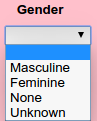
\includegraphics[width=0.148\textwidth]{gender.png}
\end{center}

But in some cases it is desirable that features of string type are also displayed as multiple
choice. For example, in the current version of Bible OL, this is possible for the features
\emph{g\_word\_nocant\_utf8}\footnote{That is, \emph{Text (no cantillation marks).}} and
\emph{g\_prs\_utf8}\footnote{That is, \emph{Pronominal suffix.}}.

A separate ``Words Database''\index{Words Database|hyperit} exists with the information necessary for this to work.

The Words Database is an SQLite3\index{SQLite3} database containing all possible values for the relevant feature.
Bible OL then constructs a drop-down box containing at most ten of the possible values, chosen at
random but guaranteed to contain the correct answer:

\begin{center}
  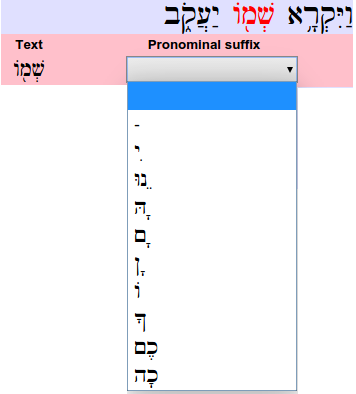
\includegraphics[width=0.4\textwidth]{pronsuf.png}
\end{center}

The strings in the drop-down box are chosen based on three keys from the \emph{objectSettings}\index{objectSettings} of
the Database Specification file. (See Section \ref{sec-objectsettings}.)

\begin{itemize}
\item The name of the Words Database, found under the \emph{alternateshowrequestDb} key.
\item An SQL statement that extracts all possible values of the feature. This is found under the
  \emph{alternateshowrequestSql} key.
\item Features to be used as parameters in the SQL statement. These are found under the
  \emph{additionalfeatures} key.\footnote{Currently, only one value is allowed in \emph{additionalfeatures.}}
\end{itemize}


Let us look at an example from the ETCBC4 database.\footnote{For a detailed description of the Words
Database for ETCBC4 see Appendix \ref{app-worddb}.} For the \emph{g\_prs\_utf8} feature (the
pronominal suffix) of the \emph{word} object, the following values are specified under
\emph{objectSettings}\index{objectSettings} in the Database Specification File:

\begin{my-tabu}{lX}{ \headii{Key}{Value} }
  additionalfeatures & \lstinline[upquote=true]|["lex"]|\\

  alternateshowrequestDb & \lstinline|ETCBC4_words.db|\\

  alternateshowrequestSql & \lstinline[upquote=true]|SELECT DISTINCT suffix FROM suffixes,lexsuf,lexemes WHERE lex='\%s' AND
  lexid=lexemes.id AND sufid=suffixes.id|\\
\end{my-tabu}

These values will direct Bible OL to replace ``\%s'' in \emph{alternateshowrequestSql} with the
value of the \emph{lex} feature retrieved from the Emdros database and then execute the SQL
statement on the \texttt{ETCBC4\_words.db} database.

In the case of the sentence \heb{וַיִּקְרָ֥א שְׁמֹ֖ו יַעֲקֹ֑ב} in the illustration above, the \emph{lex} feature
of the word \heb{שְׁמֹ֖ו} has the value ``CM/''. Bible OL will therefore execute this SQL statement:

\begin{lstlisting}[language=SQL]
SELECT DISTINCT suffix FROM suffixes,lexsuf,lexemes
    WHERE lex='CM/' AND lexid=lexemes.id AND sufid=suffixes.id
\end{lstlisting}

This will yield a collection of all possible pronominal suffixes associated with the \emph{lex}
value ``CM/''. Bible OL will then choose ten of these at random, while still ensuring that the
correct answer (\heb{ֹו}) is among them, and present them in a drop-down box.

If the SQL statement yields only a single value, it is not turned into a drop-down box as with the second
word here:

\begin{center}
  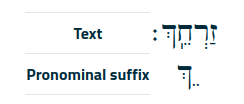
\includegraphics[width=0.4\textwidth]{pronsuf2.png}
\end{center}

%%%%%%%%%%%%%%%%%%%%%%%%%%%%%%%%%%%%%%%%%%%%%%%%%%%%%%%%%%%%%%%%%%%
%%%%%%%%%%%%%%%%%%%% Multiple-Choice Questions %%%%%%%%%%%%%%%%%%%%
\chapter{Hints}\label{chap-hints}\index{hints}

\textbf{Read this chapter if you need to understand or modify the way Bible OL hinting for some
  Hebrew verbs.}
\plainbreak{3}


In some cases, a Hebrew verb form may have several interpretations depending on the context. For
example, the word \heb{תֵרָאֶה} (\bibleref{Genesis}{1}{9}) can be either 2nd person, singular,
masculine or 3rd person, singular, feminine. A student looking merely at the word form, will not be
able to determine the correct interpretation. In the context of \bibleref{Genesis}{1}{9} the word is
3rd person, singular, feminine. A teacher can choose to display the \emph{hint} feature in exercises
to help the student select the correct interpretation. For example, \bibleref{Genesis}{1}{9} may be
displayed thus:

\begin{center}
  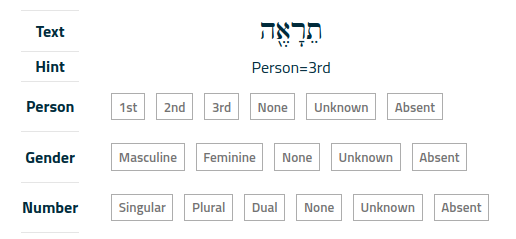
\includegraphics[width=0.6\textwidth]{hint.png}
\end{center}

A separate ``Hints Database''\index{Hints Database|hyperit} exists with the information necessary
for this to work.

The Hints Database is an SQLite3\index{SQLite3} database containing all possible values for the
relevant feature. For a detailed description of the Hints Database see Appendix \ref{app-hintsdb}.

The \emph{hint} feature is implemented as a pseudofeature (see Section \ref{sec-pseudofeature}).
Hints are only available for verbs, and only in situations where the verb form is ambiguous.


%%%%%%%%%%%%%%%%%%%%%%%%%%%%%%%%%%%%%%%%%%%%%%%%%%%%%%%%%%%%%%%%%%%%%
%%%%%%%%%%%%%%%%%%%% Client/Server Data Exchange %%%%%%%%%%%%%%%%%%%%
\chapter{Data Exchange}\label{chap-data-exchange}

\textbf{Read this chapter if you are going to work with code that accesses the Emdros databases on
  the server or displays text and exercises in the client.}
\plainbreak{3}

This chapter describes the data exchange between the client\index{client} (web browser\index{web browser})
and the server\index{server}.

%%%%%%%%%%%%%%%%%%%% Displaying Text %%%%%%%%%%%%%%%%%%%%
\section{Displaying Text}\label{displaying-text}

A user requests Bible OL to display a particular passage by accessing a URL%
\index{URL!for displaying text}
in one of these formats:

\begin{lstlisting}[frame=]
http://%\textrm{\textit{hostname}}%/text/show_text/%\textrm{\textit{dsfname}}%/%\textrm{\textit{book}}%/%\textrm{\textit{chapter}}%
http://%\textrm{\textit{hostname}}%/text/show_text/%\textrm{\textit{dsfname}}%/%\textrm{\textit{book}}%/%\textrm{\textit{chapter}}%/%\textrm{\textit{verse}}%
http://%\textrm{\textit{hostname}}%/text/show_text/%\textrm{\textit{dsfname}}%/%\textrm{\textit{book}}%/%\textrm{\textit{chapter}}%/%\textrm{\textit{firstverse}}%/%\textrm{\textit{lastverse}}%
\end{lstlisting}

The first variant retrieves an entire chapter, the second variant retrieves a single verse, and the
third variant retrieves a range of verses.

The \emph{dsfname} in the URLs is the primary name of the Database Specification File%
\index{Database Specification File}
(Section \ref{sec-dsf}); so if the \emph{dsfname} is ``ETCBC4-translit'', the
server will access the Database Specification File \texttt{ETCBC4-translit.db.json}.

So, for example, to retrieve \bibleref{Genesis}{1}{2-5} from ETCBC4-translit on the
server with hostname \texttt{bibleol.3bmoodle.dk}, you can use this URL:
\url{https://bibleol.3bmoodle.dk/text/show_text/ETCBC4-translit/Genesis/1/2/5}.

The server will always expand the requested range of verses to contain a complete set of sentences;
so a request for \bibleref{Genesis}{1}{16-17} will automatically be expanded to include verse 18,
because verses 17 and 18 comprise a single sentence.

When the server has interpreted the components of the URL, it queries the relevant Emdros database,
and based on the result it generates an HTML document containing little more than the relevant
headers, HTML code to lay out the menu, and these JavaScript variables:

\begin{my-longtabu}{lX}{ \headii{Variable}{Contents} }
  useToolTip & A Boolean value of \emph{true} if the grammar information box%
  \index{grammar information box}
  should be displayed as a tooltip\index{tooltip} under the mouse, \emph{false}
  if the grammar information box should be displayed at the right side of the browser window. This
  value is configurable on a per-user basis, but currently there is no user interface to change its
  value.\\

  configuration\hmmindex{configuration JavaScript variable@\string\emph{configuration} JavaScript variable} &
  A JavaScript object whose value is the contents of the Database Specification File
  (Section \ref{sec-dsf}).\\

  l10n\hmmindex{l10n JavaScript variable@\string\emph{l10n} JavaScript variable} &
  A JavaScript object whose value is the Grammar Localization Structure\index{Grammar Localization Structure}
  (Section \ref{sec-gram-loc-struct}).\\

  l10n\_js\hmmindex{l10n_js JavaScript variable@\string\emph{l10n\_js} JavaScript variable} & A
  JavaScript object whose key/value pairs provide localized text for the user interface. (Chapter
  \ref{chap-localize}.)\\

  typeinfo\hmmindex{typeinfo JavaScript variable@\string\emph{typeinfo} JavaScript variable} &
  A JavaScript object whose value is the contents of the Database Type Information File (Section
  \ref{sec-tif}).\\

  site\_url & The base part of the URL of the website.

  (For example, \texttt{https://bibleol.3bmoodle.dk/}.)\\

  dictionaries\hmmindex{dictionaries JavaScript variable@\string\emph{dictionaries} JavaScript variable} &
  The text to display, including grammar information. This is a JavaScript object in
  a format defined in Chapter \ref{chap-dictionary}.\\

  quizdata\hmmindex{quizdata JavaScript variable@\string\emph{quizdata} JavaScript variable} &
  This variable is \emph{null}, indicating that we are displaying text, not running an
  exercise.\\
\end{my-longtabu}

Included in the HTML document that the server sends to the client is a link to a number of CSS and
JavaScript files, including \texttt{ol.js}, which contains the main piece of code that is to run on
the client.

When the client (the web browser) has read the HTML file, the JavaScript code directs it to construct
the visual appearance of the text. This involves building the central text layout, adding
grammatical information to each word, phrase, clause, etc., and constructing the grammar selection
box\index{grammar selection box} and the grammar information box.\index{grammar information box}

%%%%%%%%%%%%%%%%%%%% Running an Exercise %%%%%%%%%%%%%%%%%%%%
\section{Running an Exercise}\index{exercise}

A user requests Bible OL to start a particular exercise by accessing a URL%
\index{URL!for running an exercise}
in one of these formats:

\begin{lstlisting}[frame=]
http://%\textrm{\textit{hostname}}%/text/show_quiz?quiz=%\textrm{\textit{excercisename}}%&count=%\textrm{\textit{numberOfQuestions}}%
http://%\textrm{\textit{hostname}}%/text/show_quiz_univ?quiz=%\textrm{\textit{excercisename}}%&count=%\textrm{\textit{numberOfQuestions}}%
\end{lstlisting}

The first variant executes an exercise based on the set of Bible passages specified in the
\xml{path} elements of the quiz template\index{quiz template}; the second variant asks the user
which Bible passages to use, and then starts the exercise. In both cases the \emph{exercisename} is
the path name (relative to the \texttt{quizzes} directory) of the file containing the exercise; the
\emph{numberOfQuestions} is a positive integer indicating the maximum number of questions to ask in
the exercise.\footnote{If \texttt{count} is omitted or if the number is illegal, five questions will
  be asked.}

So, for example, to run an exercise consisting of ten questions from the quiz template file
\texttt{Nestle~1904/demo/case.3et} on the server with hostname \texttt{bibleol.3bmoodle.dk}, you can
use this URL:
\url{https://bibleol.3bmoodle.dk/text/show_quiz?quiz=Nestle\%201904/demo/case.3et&count=10}. This
will use the pre-defined set of Bible passages stored in the quiz template file.

If the user chooses the second variant of the URL, the server will display a tree of books of the
Bible. The user can open book nodes to display a list of chapters, and they can open chapter nodes
to display a list of verses. The client retrieves the number of chapters in each book and the number
verses in each chapter as needed using AJAX requests from the \emph{jstree}\index{jstree} package
(see page \pageref{jstree}). Once the user clicks the ``Start quiz'' button%
\index{start quiz button@``Start quiz'' button},
the client sends an HTTP~POST request to the server containing the
quiz template filename, the number of questions to ask, and the list of selected passages.

The server uses information in the quiz template file and the list of passages (either the list specified
by the user or the pre-defined list from the template) to generate a query for the relevant Emdros
database. Based on the result of the query, the server generates an HTML document containing little
more than the relevant headers, HTML code to lay out the menu, and these JavaScript variables:

\begin{my-longtabu}{lX}{ \headii{Variable}{Contents} }
  useToolTip & The same as in Section \ref{displaying-text}.\\

  configuration & The same as in Section \ref{displaying-text}.\\

  l10n & The same as in Section \ref{displaying-text}.\\

  l10n\_js & The same as in Section \ref{displaying-text}.\\

  typeinfo & The same as in Section \ref{displaying-text}.\\

  site\_url & The same as in Section \ref{displaying-text}.\\

  dictionaries\hmmindex{dictionaries JavaScript variable@\string\emph{dictionaries} JavaScript variable} &
  For each question, this variable contains the text to display, including grammar
  information. This is a JavaScript object in a format defined in Chapter
  \ref{chap-dictionary}.\\

  quizdata\hmmindex{quizdata JavaScript variable@\string\emph{quizdata} JavaScript variable} &
  A JavaScript object containing information about the exercise being run. This includes
  information about the display features and the request features and their (correct) values. This
  variable is described in Chapter \ref{chap-quizdata}.\\
\end{my-longtabu}

Included in the HTML document that the server sends to the client is a link to a number of CSS and
JavaScript files, including \texttt{ol.js}, which contains the main piece of code that is to run on
the client.

When the client (the web browser) has read the HTML file, the JavaScript code directs it to
construct the visual appearance of the questions. This involves building the central text layout,
adding grammatical information to each word, phrase, clause, etc., building the question/answer
panel, and constructing the grammar selection box\index{grammar selection box} and the grammar
information box.\index{grammar information box}

As the user answers the questions, the client keeps track of the answers, but no communication with
the server takes place before the user presses the
``GRADE task''\index{grade task button@``GRADE task'' button}
or ``SAVE outcome''\index{save outcome button@``SAVE outcome'' button} button. What
happens when one of these buttons is pressed, depends on whether the user is logged in or not. If
the user not logged in, the client instructs the server to display the \emph{Select a Quiz} web
page. But if the user is logged in, the client sends the result to the server URL
\texttt{http://}\textit{hostname}\texttt{/statistics/update\_stat}, which updates the
statistics\index{statistics} for the user. The record in the user statistics table has a field
called \emph{grading}; this field is set to 0 if the user pressed the ``SAVE outcome'' button, the
field is set to 1 if the use pressed the ``GRADE task'' button. The \emph{grading} field is used by
Learning Journey (see Section \ref{sec-lj}).



%%%%%%%%%%%%%%%%%%%%%%%%%%%%%%%%%%%%%%%%%%%%%%%%%%%%%%%%%%%%%%%%%%%
%%%%%%%%%%%%%%%%%%%% The dictionaries Variable %%%%%%%%%%%%%%%%%%%%
\chapter{The \emph{dictionaries} Variable}\label{chap-dictionary}%
\index{dictionaries JavaScript variable@\emph{dictionaries} JavaScript variable|hyperit}

\textbf{Read this chapter if you are going to work with code that accesses the Emdros databases on
  the server or displays text and exercises in the client.}
\plainbreak{3}

All information about the text to display, the associated feature values, and the phrase, clause,
and sentence structure of the text is communicated between the server and the client in the
JavaScript variable \emph{dictionaries}.

This means that the primary task of the server\index{server} is to convert data from the Emdros
database into a format that can be stored in the \emph{dictionaries} variable, and the primary task
of the client\index{client} is to convert the contents of the \emph{dictionaries} variable into
displayed text.

In the PHP files executed by the server, the value is described by the \emph{Dictionary}%
\index{Dictionary PHP class@\emph{Dictionary} PHP class}
class in the file \texttt{myapp/libraries/Dictionary.php}. In the TypeScript files executed by the
client, the value is described by \emph{DictionaryIf}%
\index{DictionaryIf TypeScript interface@\emph{DictionaryIf} TypeScript interface}
interface in the file \texttt{ts/dictionary.ts}.

Note: There is also a class in the client called \emph{Dictionary}. This is not the same as the
\emph{Dictionary} class in the server (although the two are related, as we shall see in Section
\ref{sec-ol}).


%%%%%%%%%%%%%%%%%%%% The TypeScript DictionaryIf and PHP Dictionary Classes %%%%%%%%%%%%%%%%%%%%
\section{The TypeScript \emph{DictionaryIf} and PHP \emph{Dictionary} Classes}\label{sec-dictionaryif}%
\index{DictionaryIf TypeScript interface@\emph{DictionaryIf} TypeScript interface|hyperit}%
\index{Dictionary PHP class@\emph{Dictionary} PHP class|hyperit}

There is a one-to-one mapping of classes and data fields in the server and in the client, but the
names differ a little, as you can see from the following.

This is a simplified overview of the relevant TypeScript definitions in the client:

\begin{lstlisting}[language=TypeScript]
interface DictionaryIf {%\index{DictionaryIf TypeScript interface@\emph{DictionaryIf} TypeScript interface}%
    sentenceSets : MonadSet[];
    monadObjects: MonadObject[][][];
    bookTitle : string;
}

interface MonadSet {%\index{MonadSet TypeScript interface@\emph{MonadSet} TypeScript interface}%
    segments : MonadPair[];
}

interface MonadPair {%\index{MonadPair TypeScript interface@\emph{MonadPair} TypeScript interface}%
    low : number;
    high : number;
}

interface MonadObject {%\index{MonadObject TypeScript interface@\emph{MonadObject} TypeScript interface}%
    mo : MatchedObject;
    children_idds : number[];
}

interface MatchedObject {%\index{MatchedObject TypeScript interface@\emph{MatchedObject} TypeScript interface}%
    id_d : number;
    name : string;
    monadset : MonadSet;
    features : {[key : string] : string;};
    sheaf : any;
}

interface SingleMonadObject extends MonadObject {%\index{SingleMonadObject TypeScript interface@\emph{SingleMonadObject} TypeScript interface}%
    text : string;
    suffix : string;
    bcv : string[];
    bcv_loc : string;
    sameAsNext : boolean[];
    sameAsPrev : boolean[];
    pics : number[];
    urls : any[];
}

interface MultipleMonadObject extends MonadObject {%\index{MultipleMonadObject TypeScript interface@\emph{MultipleMonadObject} TypeScript interface}%
    subobjects : MatchedObject[][];
}
\end{lstlisting}

This is a simplified overview of the corresponding PHP definitions in the server:

\begin{lstlisting}[language=PHP]
class Dictionary {%\index{Dictionary PHP class@\emph{Dictionary} PHP class}%
    public $sentenceSets; // An array of OlMonadset objects
    public $monadObjects; // An array of arrays of arrays of MonadObject objects
    public $bookTitle;
}

class OlMonadSet implements Iterator {%\index{OlMonadSet PHP class@\emph{OlMonadSet} PHP class}%
    public $segments;   // An array of MonadPair objects
}


class MonadPair {%\index{MonadPair PHP class@\emph{MonadPair} PHP class}%
    public $low;
    public $high;
}

abstract class MonadObject {%\index{MonadObject PHP class@\emph{MonadObject} PHP class}%
    public $mo;         // An OlMatchedObject object
    public $children_idds;
}

class OlMatchedObject {%\index{OlMatchedObject PHP class@\emph{OlMatchedObject} PHP class}%
    public $id_d;
    public $name;
    public $monadset;   // An OlMonadSet object
    public $features;   // Maps feature name to feature value
    public $sheaf;
}


class SingleMonadObject extends MonadObject {%\index{SingleMonadObject PHP class@\emph{SingleMonadObject} PHP class}%
    public $text;
    public $suffix;
    public $bcv;        // An array of strings or integers
    public $bcv_loc;    // Localized version of bcv
    public $sameAsNext; // An array of Booleans
    public $sameAsPrev; // An array of Booleans
    public $pics;       // An array of integers
    public $urls;       // An array of string pairs
}

class MultipleMonadObject extends MonadObject {%\index{MultipleMonadObject PHP class@\emph{MultipleMonadObject} PHP class}%
    public $subobjects; // MatchedObjects for any subobjects retrieved for this MultipleMonadObject
}
\end{lstlisting}

In the following text, the names from the client definitions are used.

The fields of the \emph{DictionaryIf} interface are:


\begin{my-longtabu}{lX}{ \headii{Field}{Contents} }
sentenceSets & Each element in this array specifies a lump of text, defined by the constituent
monads. When using the ``Display text'' feature of Bible OL, \emph{sentenceSets} contains only a
single lump of text, and the array therefore has a single element. When running an exercise, each question
uses a separate lump of text, and there are as many entries in the array as there are questions in
the exercise.

\vspace{2mm}
If, for example \emph{sentenceSets[2]} has the value

\quad\texttt{\{"segments": [\{"low": 8868, "high": 8877\}]\}},

it means that the third question (index 2) is based on monads 8868-8877 from the
Emdros database.\\

monadObjects & An array of arrays of arrays of \emph{MonadObject} objects. The first index of this
array corresponds to the index in the \emph{sentenceSets} array. The second index selects the level
in the grammatical hierarchy (for example, word -- phrase -- clause -- sentence). At the third level
we find the actual objects.

\vspace{2mm}
For example, \emph{monadObjects[0][2][4]} is the \emph{MonadObject} that describes the fifth (index~4) clause
(index~2) of the first (index~0) lump of text.\\

bookTitle & The title of the current book of the Bible. It is used by the client to display an
appropriate heading on the webpage when displaying text.\\

\end{my-longtabu}

The grammatical information about each object is structured in a grammatical hierarchy%
\index{grammar hierarchy}.
At the lowest level we have \emph{words.}\index{word} The names of the objects above
the words are named \emph{phrase,}\index{phrase} \emph{clause,}\index{clause} and
\emph{sentence}\index{sentence} in ETCBC4; they are named \emph{clause level~2,}\index{clause2}
\emph{clause level~1,}\index{clause1} and \emph{sentence}\index{sentence} in nestle1904. The names
and the depth of the hierarchy can be chosen freely by the database, although the user interface can
only display a limited number of levels.

Above the top level, all sentences in a lump of text are grouped together in a so-called
``patriarch\index{patriarch|hyperit}'' object.

Each Emdros object is described by a \emph{MonadObject} in the \emph{monadObjects} array mentioned
above. The second index of \emph{monadObjects} identifies the level in the grammatical hierarchy.
\emph{MonadObject} is an abstract class, its concrete subclasses are \emph{SingleMonadObject}%
\index{SingleMonadObject TypeScript interface@\emph{SingleMonadObject} TypeScript interface}
and \emph{MultipleMonadObject}%
\index{MultipleMonadObject TypeScript interface@\emph{MultipleMonadObject} TypeScript interface}.

At the lowest level (the word level) the \emph{MonadObjects} belong to the class
\emph{SingleMonadObject,} which represents Emdros objects that correspond to a single monad\index{monad}. At the
higher levels in the grammatical hierarchy, the \emph{MonadObjects} belong to the class
\emph{MultipleMonadObject,} which represents Emdros objects that correspond to a multiple monads.

Consider, for example, the middle sentence of \bibleref{Genesis}{1}{7}:\footnote{I am using a transliterated text
  here because a left-to-right orientation will make the following illustrations easier to read.}

\begin{center}
% The character ᵃ is placed outside \emph{...} because of font problems
\emph{wayyavdēl bên hammayim ʔ}ᵃ\emph{šer mittaḥat lārāqîₐʕ ûvên hammayim ʔ}ᵃ\emph{šer mēʕal lārāqîₐʕ}\thinspace\footnote{In English: ``and separated the waters that were under the expanse from the waters that were above
the expanse.''}
\end{center}

\Needspace*{5cm}%
At grammatical level 0\index{grammar hierarchy}, the words are assigned these monads:

\begin{center}
\begin{shaded}
\begin{tabu}{@{}c|c|c|c|c|c|c|c|c|c|c@{}}
wa- & yyavdēl & bên & ha- & mmayim & ʔᵃšer & mi- & ttaḥat & lā- & - & rāqîₐʕ \\
101 & 102 & 103 & 104 & 105 & 106 & 107 & 108 & 109 & 110 & 111 \\
\end{tabu}

\vspace{5mm}

\begin{tabu}{@{}c|c|c|c|c|c|c|c|c|c@{}}
û- & vên & ha- & mmayim & ʔᵃšer & mē- & ʕal & lā- & - & rāqîₐʕ\\
112 & 113 & 114 & 115 & 116 & 117 & 118 & 119 & 120 & 121\\
\end{tabu}
\end{shaded}
\end{center}

Assuming that the \emph{dictionaries} variable contains just this one lump of text (that is,
\emph{sentenceSet} contains only one element), the 21 words are represented as
\emph{SingleMonadObjects} in \emph{monadObjects[0][0][0..20]} in the \emph{dictionaries} variable.
(The ``words'' with monads 110 and 120 a null forms of the definite article.)

At grammatical level 1\index{grammar hierarchy}, the words are grouped into phrases thus:

\begin{center}
\begin{shaded}
\begin{tabu}{@{}c|c|c|c|c|c|c@{}}
wa- & yyavdēl & bên hammayim ûvên hammayim & ʔᵃšer & mittaḥat lārāqîₐʕ & ʔᵃšer & mēʕal lārāqîₐʕ\\
101 & 102 & 103-105, 112-115 & 106 & 107-111 & 116 & 117-121\\
\end{tabu}
\end{shaded}
\end{center}

Note how the third phrase consists of two lumps of contiguous monads. The seven phrases are represented
as \emph{MultipleMonadObjects} in \emph{monadObjects[0][1][0..6]} in the \emph{dictionaries} variable.


At grammatical level 2\index{grammar hierarchy}, the phrases are grouped into clauses thus:\label{clause-example}

\begin{center}
\begin{shaded}
\begin{tabu}{@{}c|c|c@{}}
wayyavdēl bên hammayim ûvên hammayim & ʔᵃšer mittaḥat lārāqîₐʕ & ʔᵃšer mēʕal lārāqîₐʕ\\
101-105, 112-115 & 106-111 & 116-121\\
\end{tabu}
\end{shaded}
\end{center}

The three clauses are represented
as \emph{MultipleMonadObjects} in \emph{monadObjects[0][2][0..2]} in the \emph{dictionaries} variable.

At grammatical level 3\index{grammar hierarchy}, the clauses are grouped into sentences thus:

\begin{center}
\begin{shaded}
\begin{tabu}{@{}c@{}}
wayyavdēl bên hammayim ʔᵃšer mittaḥat lārāqîₐʕ ûvên hammayim ʔᵃšer mēʕal lārāqîₐʕ\\
101-121\\
\end{tabu}
\end{shaded}
\end{center}

In this example, only a single sentence is present.
This sentence is represented as a \emph{MultipleMonadObject} in \emph{monadObjects[0][3][0]} in the
\emph{dictionaries} variable.

Finally, at grammatical level 4\index{grammar hierarchy}, the sentences are grouped into a single
patriarch\index{patriarch} object. In this example the patriarch contains the same monads as the
sentence object. The patriarch is represented as a \emph{MultipleMonadObject} in
\emph{monadObjects[0][4][0]} in the \emph{dictionaries} variable.


In Bible OL the grammatical hierarchy can be displayed thus:

\begin{center}
  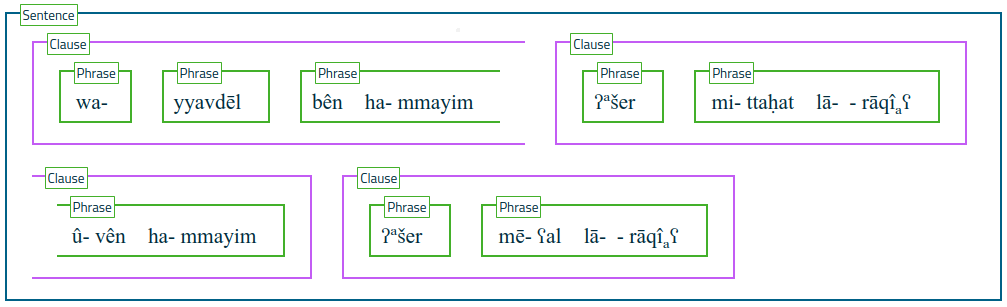
\includegraphics[width=1.0\textwidth]{gen1_7.png}
\end{center}

Note how the frames around the split phrase and clause are drawn.

%%%%%%%%%%%%%%%%%%%% The MonadObject Class and Its Subclasses %%%%%%%%%%%%%%%%%%%%
\section{The \emph{MonadObject} Class and Its Subclasses}%
\index{MonadObject TypeScript interface@\emph{MonadObject} TypeScript interface|hyperit}\label{MonadObject}

The previous section describes how objects of class \emph{MonadObject} are used to represent Emdros
objects in the \emph{monadObjects} field in the \emph{dictionaries} variable. (Strictly speaking,
\emph{MonadObject} is an interface in TypeScript and an abstract class in PHP, but that is
irrelevant to the following discussion.)

The \emph{MonadObject} class has these members:

\begin{my-tabu}{lX}{ \headii{Field}{Contents} }
mo & An object of class \emph{MatchedObject}%
     \hmmindex{MatchedObject TypeScript interface@\string\emph{MatchedObject} TypeScript interface}
     (\emph{OlMatchedObject}%
     \hmmindex{OlMatchedObject PHP class@\string\emph{OlMatchedObject} PHP class}
     in PHP). A \emph{MatchedObject} is a representation of data about a single Emdros object. Details
     are given in Section \ref{matchedobject}.\\

children\_idds & An array of integers containing the ID\_Ds\index{Emdros!ID\_D} of the constituent
                 Emdros objects at a lower level in the grammar hierarchy. Consider, for example,
                 the three clauses at grammatical level 2 in the example on page
                 \pageref{clause-example}. The clause ``ʔᵃšer mittaḥat lārāqîₐʕ'' contains the two
                 phrases ``ʔᵃšer'' and ``mittaḥat lārāqîₐʕ''. If these two phrases have ID\_Ds 357
                 and 362, then \emph{children\_idds} of the clause will be the array [~357,~362~].\\
\end{my-tabu}

At the lowest level (the word level) in the grammar hierarchy\index{grammar hierarchy}, where every
Emdros object corresponds to a single monad, the \emph{SingleMonadObject}%
\index{SingleMonadObject TypeScript interface@\emph{SingleMonadObject} TypeScript interface}
subclass of \emph{MonadObject} is used to represent an Emdros object.

In addition to the fields mentioned above, a \emph{SingleMonadObject} has these members:

\begin{my-longtabu}{lX}{ \headii{Field}{Contents} }
text & A string containing the text used to display the word.\\

suffix & A string containing the suffix feature, if any, of the word. (See Section
\ref{sec-contin}.)\\

bcv & An array containing the Bible reference for the verse containing the word. For a word in
\bibleref{Genesis}{1}{7}, \emph{bcv} is the array [~``Genesis'',~1,~7~].\\

bcv\_loc & A localized version of the Bible reference.\\

sameAsNext & An array of Booleans. \emph{sameAsNext[0]} is \emph{true} if this word belongs to the
same book\index{book} as the next word; \emph{sameAsNext[1]} is \emph{true} if this word belongs to
the same chapter\index{chapter} as the next word; \emph{sameAsNext[2]} is \emph{true} if this word
belongs to the same verse\index{verse} as the next word. For the last word in a collection, all
three Booleans are \emph{false.}\\

sameAsPrev & An array of Booleans. \emph{sameAsPrev[0]} is \emph{true} if this word belongs to the same
book as the previous word; \emph{sameAsPrev[1]} is \emph{true} if this word belongs to the same chapter as
the previous word; \emph{sameAsPrev[2]} is \emph{true} if this word belongs to the same verse as the
previous word. For the first word in a collection, all three Booleans are
\emph{false.}\\

pics & An array of integers identifying pictures on the resource website\index{resource website} (see Section
\ref{sec-resource-web}) that are relevant for this word. The first three values in the array are the book
number, chapter number, and verse number. The remaining elements are IDs of pictures on the resource
website.\\

urls & An array of references to URLs that are relevant for the word. Each entry in the array is
itself an array with two elements: the URL and a string identifying the icon to show in Bible OL. If,
for example an element in \emph{url} has the value [~``http://example.com/here.html'',~``v''~],
Bible OL will show a hyperlink to \texttt{http://example.com/here.html} in the form of a V icon.
For more information see Section
\ref{sec-resource-web}.\\
\end{my-longtabu}

In addition to the fields mentioned above, a \emph{MultipleMonadObject} has this member:

\begin{my-longtabu}{lX}{ \headii{Field}{Contents} }
  subobjects & Subobjects (for example, \emph{clause\_atom} as a subobject of \emph{clause}) in
  cases where a sentencegrammar refers to such objects.\\
\end{my-longtabu}


%%%%%%%%%%%%%%%%%%%% The MatchedObject Class %%%%%%%%%%%%%%%%%%%%
\section{The \emph{MatchedObject} Class}%
\index{MatchedObject TypeScript interface@\emph{MatchedObject} TypeScript interface|hyperit}\label{matchedobject}

A \emph{MatchedObject} (called an \emph{OlMatchedObject}%
\index{OlMatchedObject PHP class@\emph{OlMatchedObject} PHP class}
in PHP) is a representation of data about a single Emdros object. It has the following members:

\begin{my-longtabu}{lX}{ \headii{Field}{Contents} }
  id\_d & The ID\_D\index{Emdros!ID\_D} of the Emdros object\\

  name & The name of the Emdros object type.\\

  monadset & A \emph{MonadSet}%
  \hmmindex{MonadSet TypeScript interface@\string\emph{MonadSet} TypeScript interface}
  (\emph{OlMonadSet}%
  \hmmindex{OlMonadSet PHP class@\string\emph{OlMonadSet} PHP class}
  in PHP) object listing the monads belonging to this object. For example, the first clause at
  grammatical level 2 in the example on page \pageref{clause-example} is represented by this value:

  \begin{minipage}{8cm}
  \begin{verbatim}

      "monadset": {
          "segments": [
              {
                  "low": 101,
                  "high": 105
              },
              {
                  "low": 112,
                  "high": 115
              }
           ]
      }
  \end{verbatim}
  \end{minipage}\\

  features & An associative array mapping feature\index{Emdros!feature} name to feature value.\\

  sheaf & Always null. (This is used by complex MQL searches that should not occur in Bible OL.)\\
\end{my-longtabu}


%%%%%%%%%%%%%%%%%%%%%%%%%%%%%%%%%%%%%%%%%%%%%%%%%%%%%%%%%%%%%%%
%%%%%%%%%%%%%%%%%%%% The quizdata Variable %%%%%%%%%%%%%%%%%%%%
\chapter{The \emph{quizdata} Variable}\label{chap-quizdata}%
\index{quizdata JavaScript variable@\emph{quizdata} JavaScript variable|hyperit}

\textbf{Read this chapter if you are going to work with code that generates exercises on
  the server or displays exercises in the client.} 
\plainbreak{3}

All information about the questions and correct answers to an exercise is communicated between the
server and the client in the JavaScript variable \emph{quizdata}.

In the server, the data is generated by the class \emph{Quiz\_data} in the file
\texttt{myapp/\allowbreak{}libraries/\allowbreak{}Quiz\_data.php}; in the client the data is described in the TypeScript
\emph{QuizData} interface in the file \texttt{ts/quizdata.ts}. Th



%%%%%%%%%%%%%%%%%%%% The TypeScript QuizData and PHP Quiz_data Classes %%%%%%%%%%%%%%%%%%%%
\section{The TypeScript \emph{QuizData} and PHP \emph{Quiz\_data} Classes}%
\index{QuizData TypeScript interface@\emph{QuizData} TypeScript interface}%
\index{Quiz PHP class@\emph{Quiz} PHP class|hyperit}

There is a one-to-one mapping of classes and data fields in the server and in the client, but the
names differ a little, as you can see from the following.

This is a simplified overview of the relevant TypeScript definitions in the client:

\begin{lstlisting}[language=TypeScript]
interface QuizData {
    quizid       : number;
    quizFeatures : ExtendedQuizFeatures;
    desc         : string;
    maylocate    : boolean;
    sentbefore   : number;
    sentafter    : number;
    monad2Id     : number[];
    id2FeatVal   : string[][];
}

interface ExtendedQuizFeatures {%\index{ExtendedQuizFeatures TypeScript interface@\emph{ExtendedQuizFeatures} TypeScript interface}%
    showFeatures : string[];
    requestFeatures : {name : string; usedropdown : boolean; }[];
    dontShowFeatures : string[];
    dontShowObjects : { content : string; show? : string; } [];
    objectType : string;
    dontShow : boolean;
    useVirtualKeyboard : boolean;
}
\end{lstlisting}

This is a (very) simplified overview of the corresponding PHP definitions in the server:

\begin{lstlisting}[language=PHP]
class Quiz_data {
    public $quizid;
    public $quizFeatures;     // An ExtendedQuizFeatures object
    public $desc;
    public $maylocate;
    public $sentbefore;
    public $sentafter;
    public $monad2Id;         // An array of integers
    public $id2FeatVal;       // An array of arrays of strings
}

class ExtendedQuizFeatures {%\index{ExtendedQuizFeatures PHP class@\emph{ExtendedQuizFeatures} PHP class}%
    public $showFeatures;     // An array of strings
    public $requestFeatures;  // An array of string/Boolean pairs
    public $dontShowFeatures; // An array of strings
    public $dontShowObjects;  // An array of string/string pairs
    public $objectType;
    public $dontShow;
    public $useVirtualKeyboard;
}
\end{lstlisting}

In the following text, the names from the client definitions are used.

The fields of the \emph{QuizData} interface are:

\begin{my-longtabu}{lX}{ \headii{Field}{Contents} }
  
  quizid & An integer used to identify the entry in the \emph{sta\_quiz} table%
           \index{sta\_quiz table}
           in the user database\index{user database} (see Section \ref{sec-staquiz}) where
           statistics about this exercise is to be stored. If the user is not logged in,
           \emph{quizid} is -1 and statistics will not be stored.\\

  quizFeatures & An object of class \emph{ExtendedQuizFeatures}. It contains information about how
                 the exercise should be presented to the user. Details are given below.\\

  desc & The description of the exercise from the quiz template file.\\

  maylocate & A Boolean value indicating if the exercise may display a ``Locate'' checkbox to the user.\\

  sentbefore & An integer value indicating the number of context sentences to display before the
               question sentence.\\

  sentafter & An integer value indicating the number of context sentences to display after the
              question sentence.\\
  
  monad2Id & An array that maps monads\index{monad} to the ID\_Ds\index{Emdros!ID\_D} of a quiz
             object\index{quiz object (a.k.a. sentence unit)}. If a quiz object covers more
             than one word, several entries in this array will have the same value. (Note that this
             assumes that a word is not part of more than one quiz object.)\\

  id2FeatVal & An array of arrays of strings. For each quiz object, this array holds information
               about the values of the display features and the correct values of the request
               features. If, for example, a quiz object has an ID\_D of 1234, and one of the display
               or request features is \emph{case} with the value \emph{genitive}, then
               \emph{id2FeatVal[1234][\q case\q]} will have the value ``genitive''.\\

\end{my-longtabu}

The \emph{ExtendedQuizFeatures}%
\index{ExtendedQuizFeatures TypeScript interface@\emph{ExtendedQuizFeatures} TypeScript interface}
interface has these members:

\begin{center}
\begin{tabu*}{@{}lX@{}}
  \toprule
  \headii{Field}{Contents}\\\addlinespace[-1mm]
  \midrule

    showFeatures & An array of strings containing the names of the display features.\index{display feature}\\

    requestFeatures & An array of objects describing the request features.\index{request feature}
    Each object has this layout:

    \begin{minipage}{8cm}
    \begin{verbatim}

    {
        name : string;
        usedropdown : boolean;
    }
    \end{verbatim}
    \end{minipage}

    The \emph{name} field contains the name of the request feature, the \emph{usedropdown} field is
    \emph{true} if the request feature is of type string and the question should be asked as a
    multiple choice\index{multiple-choice} question (see Section \ref{chap-multiple-choice}).\\

    dontShowFeatures & Array of strings naming features that must not be available in the grammar
    selection box and the grammar information box.\index{grammar information box}\\

    dontShowObjects & An array of objects naming Emdros object types that must not be available in
    the grammar selection box and the grammar information box. Each object has this layout:

    \begin{minipage}{8cm}
    \begin{verbatim}

    {
        content : string;
        show? : boolean;
    }
    \end{verbatim}
    \end{minipage}

    The \emph{content} field contains the name of the Emdros object type, the optional \emph{show}
    names a feature of that Emdros object that may be displayed nonetheless. Currently, this is only
    used to display features that are qere forms of Hebrew words.\\

    objectType & The Emdros type of the quiz objects.\\

    dontShow & \emph{True} if the quiz objects should be replaced with (1), (2), (3), etc. in the
    displayed text.\\

    useVirtualKeyboard & \emph{True} if the client should display a virtual keyboard%
    \index{virtual keyboard}
    to facilitate the typing of text in a foreign alphabet.\\

\addlinespace[-1mm]\bottomrule
\end{tabu*}
\end{center}

The \emph{quizFeatures} field of the \emph{QuizData} interface has the additional fields
\emph{useDropdown, additionalFeatures,} and \emph{allFeatures.} They are not used by the client
software.


%%%%%%%%%%%%%%%%%%%%%%%%%%%%%%%%%%%%%%%%%%%%%%%%%%%%%%%%%%%%%%%%%%%
%%%%%%%%%%%%%%%%%%%% The CodeIgniter Framework %%%%%%%%%%%%%%%%%%%%
\chapter{The CodeIgniter Framework}\label{chap-codeigniter-use}\index{CodeIgniter|hyperit}

\textbf{Read this chapter if you are going to understand or modify the server code.}
\plainbreak{3}

Bible OL uses a PHP\index{PHP} framework known as \emph{CodeIgniter,} which provides a simple
decoding of URLs, forces a model-view-controller approach to the software structure, and provides a
large library for performing a number of tasks. Currently, Bible OL uses CodeIgniter version 3.1.7.

If you are going to modify server\index{server} code, you will need a good understanding of how
CodeIgniter works, and you should therefore read the documentation at
\url{http://www.codeigniter.com/docs}. The following sections provide a few examples of what
CodeIgniter can do for the programmer.

%%%%%%%%%%%%%%%%%%%% URL Decoding %%%%%%%%%%%%%%%%%%%%
\section{URL Decoding}\label{url-decoding}\index{URL!decoding in CodeIgniter}

When a user accesses a URL such as, for example, \texttt{http://website/aaaaa/bbb}, this will cause
CodeIgniter to call the PHP function \emph{bbb} in the class \emph{Ctrl\_aaaaa}, which is located in
the file \emph{ctrl\_aaaaa.php}.

It is also possible to access these functions from the shell command line on the server. The shell command

\begin{lstlisting}[language=bash]
php index.php aaaaa bbb
\end{lstlisting}

\noindent
is equivalent to accessing \texttt{http://website/aaaaa/bbb}.

If the function name is omitted, it defaults to \emph{index}.


%%%%%%%%%%%%%%%%%%%% Model-view-controller Structure %%%%%%%%%%%%%%%%%%%%
\section{Model-view-controller Structure}\index{model-view-controller|hyperit}\index{MVC|see {model-view-controller}}

It is customary in many large programming projects to split functionality into three groups:

\begin{list}{-}{%
    \setlength{\itemsep}{0pt}%
    \setlength{\parsep}{0pt}%
    \setlength{\topsep}{\baselineskip}%
    \setlength{\partopsep}{0pt}%
  }
  \item Models\index{model}, which are responsible for providing the data that is to be displayed to the user.
  \item Views\index{view}, which handle the actual layout on the computer screen.
  \item Controllers\index{controller}, which handle the flow of data between the models and the views.
\end{list}

CodeIgniter makes structuring PHP code into model-view-controller groups easy.

Continuing with the example from the previous section, the function \emph{bbb} contains the
\emph{controller}\index{controller} code.

This controller function may load one or model \emph{models}\index{model}. If, for example, \emph{bbb}
executes this code:

\begin{lstlisting}[language=PHP]
$this->load->model('mod_users');
$this->mod_users->get_user_by_id(8);
\end{lstlisting}

\noindent
the model class \emph{Mod\_users} is loaded from the file \emph{mod\_users.php} and the function
\emph{get\_\-user\_\-by\_\-id(8)} is called in that class. The \emph{Mod\_users} class handles the data
exchange with the underlying user database\index{user database}.

Once the controller has retrieved the relevant data, it may load a \emph{view}\index{view} class which handles
the generation of the HTML code presented to the browser. If, for example, \emph{bbb} executes
this code:

\begin{lstlisting}[language=PHP]
$this->load->view('view_main_page', array('name' => $user_name,
                                          'email' => $user_email));
\end{lstlisting}

\noindent
the view file \emph{view\_main\_page.php} will be loaded and the variables \texttt{\$user\_name} and
\texttt{\$user\_email} will be transferred to the file. The code in the view file (mostly HTML) will
then be sent to the browser.

%%%%%%%%%%%%%%%%%%%%% Library Functions %%%%%%%%%%%%%%%%%%%%%%%%
\section{Library Functions}

The CodeIgniter library provides a large set of library functions. One of the most important is a
set of functions that enable easy and safe construction of SQL\index{SQL} statements. For example,
instead of the PHP/SQL statement

\begin{lstlisting}[language=SQL]
SELECT * from {$db_prefix}user WHERE name=$username AND age=$userage ORDER BY id;
\end{lstlisting}

\noindent
you can write this PHP code:

\begin{lstlisting}[language=PHP]
$this->db->select('*')
     ->from('user')
     ->where('name', $username)
     ->where('age', $userage)
     ->order_by('id');
\end{lstlisting}

%%%%%%%%%%%%%%%%%%%% Adding Code %%%%%%%%%%%%%%%%%%%%
\section{Adding Code}

Almost all PHP code resides in the directory \texttt{myapp}. Controller\index{controller},
model\index{model}, and view\index{view} classes are found in the directories
\texttt{myapp/controllers}, \texttt{myapp/models}, and \texttt{myapp/views}, respectively. Functions
can be added to existing classes, or files containing new classes can be added to the
subdirectories.

The code for CodeIgniter itself resides in the directory \texttt{CodeIgniter}.

CodeIgniter is configured through definitions in the files located in the directory
\texttt{myapp/config}. I have added a file \texttt{ol.php}\index{ol.php} to this directory
containing these configuration variables:

\begin{my-tabu}{lX}{ \headii{Index in \$config}{Value} }
pw\_salt & Salt\index{salt} for storing the password in the user database\index{user database}.\\

mql\_driver & Set to \texttt{'native'} to select a built-in MQL driver\index{MQL driver}. Set to or
\texttt{'extern'} to run MQL commands external to the PHP interpreter.\\

mail\_sender\_address & The sender\index{email address} address on email sent by Bible OL to
registered users.\\

mail\_sender\_name & The sender\index{email sender} name on email sent by Bible OL to registered
users.\\

google\_client\_id & Used by Google login\index{login!Google} (see Section \ref{sec-oauth-login}).\\

google\_client\_secret & Used by Google login\index{login!Google} (see Section \ref{sec-oauth-login}).\\

facebook\_client\_id & Used by Facebook login\index{login!Facebook} (see Section \ref{sec-oauth-login}).\\

facebook\_client\_secret & Used by Facebook login\index{login!Facebook} (see Section \ref{sec-oauth-login}).\\
\end{my-tabu}



%%%%%%%%%%%%%%%%%%%%%%%%%%%%%%%%%%%%%%%%%%%%%%%%%%%%%
%%%%%%%%%%%%%%%%%%%% Server Code %%%%%%%%%%%%%%%%%%%%
\chapter{Server Code}\label{chap-server-code}\index{server}

\textbf{Read this chapter if you are going to understand or modify the server code.}
\plainbreak{3}

This chapter describes some of the techniques and tools you will find in the server code. The server
code is written in PHP\index{PHP}, and almost all the server code resides in the directory
\texttt{myapp}. The server code uses the CodeIgniter\index{CodeIgniter} framework (see Section
\ref{chap-codeigniter-use}), and a good understanding of how CodeIgniter works is essential to
understanding the server code.

%%%%%%%%%%%%%%%%%%%% Models, Views, and Controllers %%%%%%%%%%%%%%%%%%%%
\section{Models, Views, and Controllers}\index{model-view-controller}

Almost all PHP code used by the server resides in the directory \texttt{myapp}. The directories
\texttt{models}, \texttt{views}, and \texttt{controllers} hold the main components of the MVC
structure supported by CodeIgniter.

The following controllers\index{controller} exist:

\begin{my-longtabu}{lX}{ \headii{Name}{Function} }

classes & Manages classes (that is, groups of users).\\

config & Allows users to change their font preferences.\\

file\_manager & Management of files and directories in the \texttt{quizzes} directory.\\

lang & Switches user interface language.\\

login & Handles login using the local\index{login!local} user database\index{user database}.\\

main\_page & Displays the main page.\\

maketypeinfo & This controller can only be accessed from the command line, not through the web
interface. It is used to create the Database Type Information File as described in Section
\ref{sec-tif}.\\

migrate & Handles upgrading from one version of Bible OL to another.\\

oauth2 & Handles login using a Google or Facebook\index{login!Google}\index{login!Facebook} account.\\

pic2db & This controller can only be accessed from the command line, not through the web interface.
It is used to retrieve information from the resource website\index{resource website} (see Section
\ref{sec-resource-web}).\\

privacy & Displays the privacy policy.\\

shebanq & Handles import of MQL from the SHEBANQ website (see Section \ref{sec-shebanq-import}).\\

statistics & Updates and displays statistics\index{statistics} about the exercises executed by the
user.\\

text & Displays text or exercises. Also handles editing of exercises.\\

translate & Allows translators to provide localization of Bible OL.\\

upload & Receives and stores uploaded exercises.\\

urls & Manages hyperlinks associated with lexemes.\\

userclass & Manages a user's relationship to a class.\\

users & Manages users.\\
\end{my-longtabu}


\Needspace*{5cm}%
The following models\index{model} exist:

\begin{my-longtabu}{lX}{ \headii{Name}{Function} }
mod\_askemdros & Retrieves Emdros-related data.\\
mod\_classdir & Manages class permissions for an exercise directory.\\
mod\_classes & Manages classes (that is, groups of users).\\
mod\_config & Manages users' font\index{font} preferences.\\
mod\_intro\_text & Generates the text on the front page.\\
mod\_localize & Generates localization information for JavaScript code (see Section \ref{sec-localize-javascript}).\\
mod\_quizpath & Exercise directory operations.\\
mod\_statistics & Manages user statistics.\index{statistics}\\
mod\_translate & Manages translating Bible OL into different languages.\\
mod\_urls & Manages hyperlinks associated with lexemes.\\
mod\_userclass & Manages a user's relationship to a class.\\
mod\_users & Manages users.\\
\end{my-longtabu}

There is no reason to go through the various views\index{view} here. Their function is best learned
by looking for calls like \texttt{\$this->load->view(...)} in the controller code.

In addition to the model/view/controller classes, the following modules are worth
noting:\footnote{Note that the list is not complete. Consult the comments in the individual files
  for more information.}

\begin{my-longtabu}{>{\ttfamily\footnotesize}lX}{ \headii{\textrm{\normalsize File}}{Contents} }
core/MY\_Controller.php & Customized version of CodeIgniter's \emph{CI\_Controller} class.\\

helpers/quiztemplate\_helper.php & XML\index{XML} parser for quiz template files.\\

helpers/sheaf\_helper.php & Classes that model data in Emdros replies.\\

helpers/sheaf\_xml\_helper.php & XML\index{XML} parser for Emdros replies.\\

helpers/xmlhandler\_helper.php & Superclass and functions for XML\index{XML} parser.\\

libraries/DB\_config.php & Classes for handling Emdros Database Description Files.\\

libraries/Dictionary.php & The \emph{Dictionary}%
\hmmindex{Dictionary PHP class@\string\emph{Dictionary} PHP class}
class (see Chapter \ref{chap-dictionary}).\\

libraries/include/dataexception.inc.php & Exception classes.\\

libraries/include/monadobject.inc.php & The \emph{MonadObject}%
\hmmindex{MonadObject PHP class@\string\emph{MonadObject} PHP class}
class and its subclasses (see Section \ref{MonadObject}).\\

libraries/include/typeinfo.inc.php & The \emph{TypeInfo}%
\hmmindex{TypeInfo PHP class@\string\emph{TypeInfo} PHP class}
class (see Section \ref{sec-tif}).\\

libraries/Mql/Mql.php & The \emph{Mql} class which handles MQL\index{MQL} requests (see Section \ref{sec-mql-server}).\\

libraries/Mql/drivers/Mql\_extern.php & Driver for executing MQL\index{MQL driver!external} commands through an external MQL
command.\\

libraries/Mql/drivers/Mql\_native.php & Driver for executing MQL commands through an MQL
library\index{MQL driver!native} in PHP.\\

libraries/picdb.php & Class for retrieving picture references and URL references from the resource
website\index{resource website} (see Section \ref{sec-resource-web}).\\

libraries/Quiz\_data.php & The \emph{Quiz\_data}%
\hmmindex{Quiz PHP class@\string\emph{Quiz} PHP class}
class and associated functions and class (see Chapter \ref{chap-quizdata}).\\

libraries/Suggest\_answers.php & Class for accessing the Words Database\index{Words Database} (see Chapter \ref{chap-multiple-choice}).\\

libraries/Universe\_tree.php & Classes used together with \emph{jstree}\index{jstree} (see page
\pageref{jstree}) to display a hierarchy of books, chapters, and verses of the Bible.\\
\end{my-longtabu}



%%%%%%%%%%%%%%%%%%%% MQL Requests in the Server %%%%%%%%%%%%%%%%%%%%
\section{MQL Requests in the Server}\label{sec-mql-server}\index{MQL driver}

The server code can be configured to execute MQL\index{MQL} requests in one of two ways:

\begin{itemize}
\item Adding an MQL library to PHP and calling the MQL API directly from PHP.
\item Executing the command line version of MQL from within PHP code.
\end{itemize}

A driver layer in Bible OL protects the programmer for having to worry about this in most cases;
this is described in Section \ref{sec-mql-if}. Information about the two drivers are found in Sections
\ref{sec-mql-native} and \ref{sec-mql-extern}.


\subsection{The MQL Interface to Bible OL}\label{sec-mql-if}

The Driver Library mechanism of CodeIgniter is used to hide the MQL implementation from the
programmer in most situations. The programmer must specify the desired way to interact with MQL by
setting \emph{\$config[\q mql\_driver\q]} in \texttt{myapp/config/ol.php}\index{ol.php} to either
\emph{\q native\q}\index{MQL driver!native} (for using the MQL PHP library) or \emph{\q extern
  \q}\index{MQL driver!external} (for using an external MQL command).

The programmer can access MQL in the following way. First, the appropriate MQL driver must be
loaded:

\begin{lstlisting}[language=PHP]
$this->load->driver('mql',array('db' => $this->db_config->emdros_db,
                                'driver' => $this->config->item('mql_driver')));
\end{lstlisting}

This is typically done in the \emph{setup} function of the \emph{mod\_askemdros} module. Here,
\emph{\$this->db\_config\allowbreak{}->emdros\_db} is the name of the Emdros database.

After this, MQL requests can be executed like in this example:

\begin{lstlisting}[language=PHP]
$emdros_data = $this->mql->exec("SELECT ALL OBJECTS WHERE [word sp=subs GET text] GOqxqxqx");
\end{lstlisting}

It is important that each Emdros command be terminated by ``GOqxqxqx'' rather than simply ``GO''. The
reason is that the MQL driver needs to split a string of several Emdros commands into individual
commands. It does this by looking for the string ``GOqxqxqx''. If the string ``GO'' had been used
instead, the occurrence of a ``GO'' inside an MQL command would cause the command splitting to fail.
The string ``GOqxqxqx'' is chosen because it is highly unlikely to occur inside an MQL command.

The call to the \emph{exec} function executes the MQL command and returns the result as an array of
\emph{TableOrSheaf} objects. The \emph{TableOrSheaf} class is defined in
\texttt{myapp/helpers/sheaf\_helper.php}.

If the result of the MQL query is a table, the \emph{get\_table} function of \emph{TableOrSheaf}
will return the table as an \emph{OlTable} object.  This object has functions
such as \emph{rows, cols, get\_header} and \emph{get\_cell} which allow you to
access various parts of the table.

If the result of the MQL query is a sheaf or a flat sheaf, the \emph{get\_sheaf} function of
\emph{TableOrSheaf} will return the table as an \emph{OlSheaf} object. This object has functions
such as \emph{get\_straws, get\_first\_straw,} and \emph{number\_of\_straws} which allow you to
access the straws within the sheaf.

\pfbreak

If you know that the MQL request will return a sheaf and you are only interested in the monads of
that sheaf, the so-called ``quick harvest\index{quick harvest}'' method can be used. In
this case you must add a Boolean argument with the value \emph{true} to the call to \emph{exec}:

\begin{lstlisting}[language=PHP]
$emdros_data = $this->mql->exec("SELECT ALL OBJECTS WHERE [word sp=subs] GOqxqxqx", true);
\end{lstlisting}

As before, \emph{exec} returns an array of \emph{TableOrSheaf} objects, but in this case all the
objects represent sheafs. As before, calling \emph{get\_sheaf} on one of these objects returns an
\emph{OlSheaf} object, but in this case the \emph{OlSheaf} only contains \emph{OlMonadSet} objects, and the
functions for accessing straws do not work. The function \emph{has\_monadset} returns \emph{true} if
any \emph{OlMonadSets} are available; and the function \emph{get\_monadset} returns an array of
\emph{OlMonadSets}.

\subsection{Driver for Native MQL}\label{sec-mql-native}\index{MQL driver!native|hyperit}

The driver for native MQL assumes that MQL support has been added to PHP. Section
\ref{sec-install-emdros} explains how to do this.

Using the native MQL driver, the MQL API is available directly from within PHP. A C++\index{C++}
version of the MQL API is described in the Emdros\index{Emdros} Programmer's Reference
Guide\footnote{\url{http://emdros.org/progref/current}}.

\subsection{Driver for External MQL}\label{sec-mql-extern}\index{MQL driver!external|hyperit}

The driver for external MQL relies on the existence of an MQL command line tool on the server. The
driver (located in file \texttt{myapp/libraries/Mql/drivers/Mql\_extern.php}) contains this variable
definition:

\begin{lstlisting}[language=PHP]
private $command_line = '/usr/local/bin/mql --xml';
\end{lstlisting}

If the MQL command line program is located in some other directory, this variable definition must be
changed accordingly.

Note that there is almost no error reporting from MQL when the external MQL command is used.


%%%%%%%%%%%%%%%%%%%% Google and Facebook Login %%%%%%%%%%%%%%%%%%%%
\section{Google and Facebook Login}\label{sec-oauth-login}\index{login!Google|hyperit}\index{login!Facebook|hyperit}\index{login!OAuth2|hyperit}

The server provides two different login mechanism. One uses a local\index{login!local} list of users
(see Section \ref{sec-user-table}), the other relies on a user's Google or Facebook login. Both
Google and Facebook provide authentication using the OAuth~2 protocol.

Google's description of how their OAuth implementation works can be found here:
\url{https://developers.google.com/accounts/docs/OAuth2WebServer}. Facebook's implementation works
in a similar manner.

The following is a brief description of the mechanism as it is set up on the Bible OL installation
that runs at \url{https://bibleol.3bmoodle.dk}.

\subsection*{Step 1. The Browser Sends Authentication Request to Google or Facebook}

\subsubsection*{Google:}

When a user clicks ``Sign in with Google+'' on the login page, the browser sends an HTTP GET request
to \texttt{https://accounts.google.com/o/oauth2/auth} with the following GET parameters:

\begin{my-tabu}{lp{10cm}}{ \headii{Name}{Value} }
response\_type & \texttt{'code'}\\
client\_id     & Our Google client ID\index{Google!client ID}, configured in the file
                 \texttt{myapp/\allowbreak{}config/\allowbreak{}ol.php}\index{ol.php}.\\
redirect\_uri  & \texttt{'https://bibleol.3bmoodle.dk/oauth2/google\_callback'}\\
scope          & \texttt{'https://www.googleapis.com/auth/userinfo.profile https://www.googleapis.com/auth/userinfo.email'}\\
state          & A random value, stored in CodeIgniter's session mechanism.\\
\end{my-tabu}

\subsubsection*{Facebook:}

When a user clicks ``Sign in with Facebook'' on the login page, the browser sends an HTTP GET request
to \texttt{https://www.facebook.com/dialog/oauth} with the following GET parameters:

\begin{my-tabu}{lp{10cm}}{ \headii{Name}{Value} }
response\_type & \texttt{'code'}\\
client\_id     & Our Facebook app ID\index{Facebook!app ID}, configured in the file
                 \texttt{myapp/\allowbreak{}config/\allowbreak{}ol.php}\index{ol.php}.\\
redirect\_uri  & \texttt{'https://bibleol.3bmoodle.dk/oauth2/facebook\_callback'}\\
scope          & \texttt{'email'}\\
state          & A random value, stored in CodeIgniter's session mechanism.\\
\end{my-tabu}


\subsection*{Step 2. Google/Facebook Responds}

Google or Facebook checks if the user can be logged in to Bible OL. Google/Facebook then sends a response to the browser,
directing it to send a new HTTP GET command to the \emph{redirect\_uri} specified in the request
above. The parameters for the new GET request depend on whether Google/Facebook approved access or not.


\subsection*{Step 3. Browser Sends Authentication Information to the Bible OL Server}

As directed by the response from Google or Facebook, the browser sends an HTTP GET request to
\texttt{https://bibleol.3bmoodle.dk/oauth2/*\_callback} with the following GET parameters:

\begin{my-tabu}{ll}{ \headii{Name}{Value} }
error & Error information if access is denied. If access is approved, this parameter is not present.\\
state & The value of the \emph{state} parameter from Step 1.\\
code & An authentication code generated by Google/Facebook.\\
\end{my-tabu}


\subsection*{Step 4. The Bible OL Server Requests an Access Token from Google/Facebook}

In Bible OL, the request from the browser is handled by the function \emph{callback} in the
\emph{Ctrl\_oauth2} controller (in the file \texttt{myapp/controllers/ctrl\_oauth2.php}). 

\subsubsection*{Google:}

If Google approved access, Bible OL does not respond immediately to the client, but sends an HTTP
POST request to \texttt{https://accounts.google.com/o/oauth2/token} with the following POST
parameters:

\begin{my-tabu}{ll}{ \headii{Name}{Value} }
code           & The authentication code received in the \emph{code} parameter in Step 3.\\
client\_id     & Our Google client ID\index{Google!client ID}, configured in the file
                 \texttt{myapp/config/ol.php}\index{ol.php}.\\
client\_secret & Our Google client secret\index{Google!client secret}, configured in the file \texttt{myapp/config/ol.php}.\\
redirect\_uri  & \texttt{'https://bibleol.3bmoodle.dk/oauth2/google\_callback'}\\
grant\_type    & \texttt{'authorization\_code'}\\
\end{my-tabu}

In response to the HTTP POST request, Google replies with a JSON string containing an
\emph{access\_token}.

\subsubsection*{Facebook:}

If Facebook approved access, Bible OL does not respond immediately to the client, but sends an HTTP
GET request to \texttt{https://graph.facebook.com/v2.4/oauth/access\_token} with the following GET
parameters:

\begin{my-tabu}{ll}{ \headii{Name}{Value} }
code           & The authentication code received in the \emph{code} parameter in Step 3.\\
client\_id     & Our Facebook app ID\index{Facebook!app ID}, configured in the file
                 \texttt{myapp/config/ol.php}\index{ol.php}.\\
client\_secret & Our Facebook app secret\index{Facebook!app secret}, configured in the file \texttt{myapp/config/ol.php}.\\
redirect\_uri  & \texttt{'https://bibleol.3bmoodle.dk/oauth2/facebook\_callback'}\\
\end{my-tabu}

In response to the HTTP GET request, Google replies with a JSON string containing an
\emph{access\_token}.


\subsection*{Step 5. The Bible OL Server Requests User Information from Google/Facebook}

\subsubsection*{Google:}

The Bible OL server sends an HTTP GET request to
\texttt{https://www.googleapis.com/oauth2/\allowbreak{}v1/\allowbreak{}userinfo} with the following
GET parameter:

\begin{my-tabu}{ll}{ \headii{Name}{Value} }
access\_token & The \emph{access\_token} received from Google in Step 4.\\
\end{my-tabu}

In response to this request, Google replies with a JSON string containing \emph{id, given\_name,
  family\_name,} and \emph{email} for the user. If this is the first time the user logs in to Bible
OL, the user information is stored in the user table\index{user table} (Section
\ref{sec-user-table}) of the user database\index{user database}. Bible OL generates a username by
concatenating the string ``ggl\_'' with the user \emph{id} received from Google.


\subsubsection*{Facebook:}

The Bible OL server sends an HTTP GET request to
\texttt{https://graph.facebook.com/v2.4/me} with the following
GET parameters:

\begin{my-tabu}{ll}{ \headii{Name}{Value} }
access\_token & The \emph{access\_token} received from Google in Step 4.\\
appsecret\_proof & A SHA256 hash of the \emph{access\_token} and the Facebook app secret.\\
fields & \texttt{'id,first\_name,last\_name,email'}\\
\end{my-tabu}

In response to this request, Facebook replies with a JSON string containing \emph{id, first\_name,
  last\_name,} and \emph{email} for the user. If this is the first time the user logs in to Bible
OL, the user information is stored in the user table\index{user table} (Section
\ref{sec-user-table}) of the user database\index{user database}. Bible OL generates a username by
concatenating the string ``fcb\_'' with the user \emph{id} received from Facebook.

\subsection*{Step 6. User is Logged In}

The Bible OL server now responds to the request sent by the browser in Step 3. The response consists
of web page informing the user that they are now logged in to the system.

\section{Account Expiry}

A cron\index{cron job} job must be set up to run daily. The cron entry must execute this command:

\begin{lstlisting}[language=bash,basicstyle={\ttfamily}]
php index.php users expire_users
\end{lstlisting}

This command calls the \emph{expire\_users} function in the \emph{Ctrl\_users} controller (in the
file \texttt{myapp/\allowbreak{}controllers/\allowbreak{}ctrl\_users.php}). The function does four
things:

\begin{itemize}
\item If a user has not logged in 48 hours after creating an account, the account is deleted.
\item If a user has not logged in for nine months, the system emails them a warning.
\item If a user has not logged in for seventeen months, the system emails them a warning.
\item If a user has not logged in for eighteen months, the account is deleted.
\end{itemize}



%%%%%%%%%%%%%%%%%%%%%%%%%%%%%%%%%%%%%%%%%%%%%%%%%%%%%%%
%%%%%%%%%%%%%%%%%%%% User Database %%%%%%%%%%%%%%%%%%%%
\chapter{User Database}\label{chap-user-database}\index{user database|hyperit}

\textbf{Read this chapter if you are going to set up a server installation or if you are going to
  use the user database}
\plainbreak{3}

The user database is a MySQL database that contains information about

\begin{itemize}
\item Users and classes registered on the system,
\item Statistics about exercises,
\item Localization strings,
\item URLs linked to glosses.
\end{itemize}


\section{Languages and Variants}\label{sec-variants}\index{variants}

When using the Bible OL website, users can select a local \emph{language} and, optionally, a
\emph{variant}. The language setting is used to select which natural language (such as, English,
German, or French) should be used for the interface. The variants allow several different versions of
the same natural language. For example, the normal English name for a particular Hebrew verb
tense may be ``Wayyiqtol'', but a variant may give the English name as ``Consecutive imperfect''.

So the different variants control the localization of the interface, the grammar terms, and the
lexicons.

When a user has selected a variant, that variant is said to be ``active''.

\section{User Database tables}


The user database contains these tables:

\begin{center}
\begin{tabu}{l@{\hspace{1cm}}l@{\hspace{1cm}}l}
alphabet              & language\_LANG                  & personal\_font         \\
bible\_refs           & language\_LANG\_VARIANT         & sta\_displayfeature    \\
bible\_urls           & lexicon\_Aramaic                & sta\_question          \\
class                 & lexicon\_Aramaic\_LANG          & sta\_quiz              \\
classexercise         & lexicon\_Aramaic\_LANG\_VARIANT & sta\_quiztemplate      \\
db\_localize          & lexicon\_greek                  & sta\_requestfeature    \\
db\_localize\_VARIANT & lexicon\_greek\_LANG            & sta\_universe          \\
exercisedir           & lexicon\_greek\_LANG\_VARIANT   & translation\_languages \\
exerciseowner         & lexicon\_Hebrew                 & user                   \\
font                  & lexicon\_Hebrew\_LANG           & userclass              \\
heb\_urls             & lexicon\_Hebrew\_LANG\_VARIANT  & userconfig             \\
language\_comment     & migrations                      &                        \\
\end{tabu}
\end{center}

The characters ``LANG'' in the names above should be replaced with language codes, such as ``en''
for English or ``da'' for Danish. The charaters ``VARIANT'' int the names above should be replaced
with the names of the available variants; if no variants are available, the variant database tables
do not exist.

Additionally, the user database contains these tables that are used by Learning Journey (see Section \ref{sec-lj}):

\begin{center}
\begin{tabu}{l@{\hspace{1cm}}l@{\hspace{1cm}}l@{\hspace{1cm}}l}
sta\_grading & sta\_gradingfeature & sta\_gradingpath & sta\_grading\_system \\
\end{tabu}
\end{center}

The names are typically prefixed by a common text string found in
\emph{\$db[\q default\q][\q dbprefix\q]} in the file \texttt{myapp/config/database.php}. If that
value is \emph{`bol\_',} the database tables will be named \emph{bol\_alphabet,
  bol\_bible\_refs} etc.

The tables (except for those used by Learning Journey) are described in the following sections.

%%%%%%%%%%%%%%%%%%%% The user Table %%%%%%%%%%%%%%%%%%%%
\section{The \emph{user} Table}\label{sec-user-table}\index{user table|hyperit}

The \emph{user} table contains information of each registered user. It has the following fields:


\begin{my-longtabu}{>{\itshape}lll}{ \headiii{\textup{Column}}{Type}{Contents} }
  id                  & Integer       & Unique number identifying the user.                     \\
  first\_name         & Text          & User's first name.                                      \\
  last\_name          & Text          & User's last name                                        \\
  family\_name\_first & Boolean       & True if Chinese name order is used.                     \\
  username            & Text          & Name used when logging in.                              \\
  password            & Text          & Encrypted password.                                     \\
  reset               & Text          & Password reset code.                                    \\
  reset\_time         & Integer       & UNIX time when password reset code was issued.          \\
  isadmin             & Boolean       & User is an administrator.                               \\
  isteacher           & Boolean       & User is a teacher.                                      \\
  istranslator        & Boolean       & User is a translator.                                   \\
  email               & Text          & User's email address.                                   \\
  oauth2\_login       & Text          & OAuth~2 service used to log user in.                    \\
  created\_time       & Integer       & UNIX time when the account was created.                 \\
  last\_login         & Integer       & UNIX time when the user last logged in.                 \\
  warning\_sent       & Integer       & Number of email warnings sent about account inactivity. \\
  preflang            & Text          & User's preferred language.                              \\
  prefvariant         & Text          & User's preferred variant.                               \\
  accept\_policy      & Integer       & UNIX time when the user accepted the privacy policy.    \\
  policy\_lang        & Text          & The language of the accepted privacy policy.            \\
  acc\_code           & Text          & Used in the policy acceptance handshake.                \\
  acc\_code\_time     & Integer       & UNIX time when \texttt{acc\_code} was generated.        \\
\end{my-longtabu}

Local users have their username and password stored in this table. Their \emph{oauth2\_login} field
is set to \emph{NULL} (0).\index{login!local}

Google users have usernames such as ``ggl\_106440263559736360192'', where 106440263559\-736\-360192 is
the user ID provided by Google. Their \emph{oauth2\_login} field is set to \emph{``google''}.\index{login!Google}

Facebook users have usernames such as ``fcb\_10206545794576996'', where 10206545794576996 is
the user ID provided by Facebook. Their \emph{oauth2\_login} field is set to \emph{``facebook''}.\index{login!Facebook}

The \emph{preflang} field is specified as either the two-letter ISO~639-1 code of the
language\footnote{For example, ``en'' for English and ``da'' for Danish.} or ``none'' for no preferred
language.

The \emph{prefvariant} field is specified as either the name of the preferred variant, ``main''
for the main variant, or ``none'' for no preferred variant.

%%%%%%%%%%%%%%%%%%%% The class Table %%%%%%%%%%%%%%%%%%%%
\section{The \emph{class} Table}\index{class table}

The \emph{class} table contains information of each class (as in ``school class'', a group of
students). It has the following fields:

\begin{my-longtabu}{>{\itshape}llX}{ \headiii{\textup{Column}}{Type}{Contents} }
  id             & Integer  & Unique number identifying the class.\\
  classname      & Text     & Name of the class.\\
  password       & Text     & An optional password required when a student enrols in a class.\\
  enrol\_before  & Date     & An optional deadline for enrolment.\\
  ownerid        & Integer  & The \emph{id} field from an entry in the \emph{user} table.
                              This field identifies the user who owns the class. Typically, this is
                              the teacher who created the class. A field value of zero means that
                              nobody owns the class.
\end{my-longtabu}

%%%%%%%%%%%%%%%%%%%% The userclass Table %%%%%%%%%%%%%%%%%%%%
\section{The \emph{userclass} Table}\index{userclass table}

An entry in the \emph{userclass} table indicates that a particular user is a member of a particular
class. The table has these fields:

\begin{my-longtabu}{>{\itshape}llX}{ \headiii{\textup{Column}}{Type}{Contents} }
 id       & Integer  & Unique number identifying this entry.\\
 userid   & Integer  & The \emph{id} field from an entry in the \emph{user} table.\\
 classid  & Integer  & The \emph{id} field from an entry in the \emph{class} table.\\
 access   & Boolean  & \emph{True} if the user has granted the class owner access to results that
 are marked as not intended for grading.\\
\end{my-longtabu}

%%%%%%%%%%%%%%%%%%%% The userconfig Table %%%%%%%%%%%%%%%%%%%%
\section{The \emph{userconfig} Table}\index{userconfig table}

The \emph{userconfig} table holds information about the configuration for a particular user.
Currently, only one option is available, and there is no user interface for configuring it. The
table has these fields:

\begin{my-longtabu}{>{\itshape}llX}{ \headiii{\textup{Column}}{Type}{Contents} }
 user\_id   & Integer  & The \emph{id} field from an entry in the \emph{user} table.\\
 usetooltip & Boolean  & \emph{True} if the user wants the grammar information box\index{grammar information box} to work as a
                          tooltip\index{tooltip} instead of having a fixed position on the display.\\
\end{my-longtabu}

%%%%%%%%%%%%%%%%%%%% The alphabet Table %%%%%%%%%%%%%%%%%%%%
\section{The \emph{alphabet} Table}\index{alphabet table}

The \emph{alphabet} table contains a list of the foreign alphabets used by Bible OL. It has the
following fields:

\begin{my-longtabu}{>{\itshape}llX}{ \headiii{\textup{Column}}{Type}{Contents} }
 id         & Integer   & Unique number identifying the alphabet.\\
 name       & Text      & The internal name of the alphabet.\\
 direction  & Text      & ``rtl'' for right-to-left text, ``ltr'' for left-to-right text.\\
 sample     & Text      & A sample text in the alphabet. This will be displayed when the user chooses fonts.\\
 english    & Text      & The English name of the alphabet.\\
\end{my-longtabu}


%%%%%%%%%%%%%%%%%%%% The font Table %%%%%%%%%%%%%%%%%%%%
\section{The \emph{font} Table}\index{font table}

The \emph{font} table contains the users' font\index{font} preferences for various alphabets. It has the
following fields:

\begin{my-longtabu}{>{\itshape}lll}{ \headiii{\textup{Column}}{Type}{Contents} }
id              & Integer & Unique number identifying this entry.\\
user\_id        & Integer & The \emph{id} field from an entry in the \emph{user} table.\\
alphabet\_id    & Integer & The \emph{id} field from an entry in the \emph{alphabet} table.\\
font\_family    & Text    & A comma-separated string of font names.\\
text\_size      & Integer & Font size when displaying text.\\
text\_italic    & Boolean & \emph{True} if the font is italic when displaying text.\\
text\_bold      & Boolean & \emph{True} if the font is bold when displaying text.\\
feature\_size   & Integer & Font size for interlinear text.\\
feature\_italic & Boolean & \emph{True} if the font is italic for interlinear text.\\
feature\_bold   & Boolean & \emph{True} if the font is bold for interlinear text.\\
tooltip\_size   & Integer & Font size for text in the grammar information box.\index{grammar information box}\\
tooltip\_italic & Boolean & \emph{True} if the font is italic for text in the grammar information box.\\
tooltip\_bold   & Boolean & \emph{True} if the font is bold for text in the grammar information box.\\
input\_size     & Integer & Font size in input fields.\\
input\_italic   & Boolean & \emph{True} if the font is italic in input fields.\\
input\_bold     & Boolean & \emph{True} if the font is bold in input fields.\\
\end{my-longtabu}

%%%%%%%%%%%%%%%%%%%% The personal_font Table %%%%%%%%%%%%%%%%%%%%
\section{The \emph{personal\_font} Table}\index{personal\_font table}

Each user can specify one personal font\index{font} per alphabet. The personal font is listed on the font
selection page together with the system fonts.

The \emph{personal\_font} table contains a user's personal fonts for a specific alphabet. It has the
following fields:

\begin{my-tabu}{>{\itshape}lll}{ \headiii{\textup{Column}}{Type}{Contents} }
id              & Integer & Unique number identifying this entry.\\
user\_id        & Integer & The \emph{id} field from an entry in the \emph{user} table.\\
alphabet\_id    & Integer & The \emph{id} field from an entry in the \emph{alphabet} table.\\
font\_family    & Text    & The name of the font.\\
\end{my-tabu}

%%%%%%%%%%%%%%%%%%%% The exercisedir and classexercise Tables %%%%%%%%%%%%%%%%%%%%
\section{The \emph{exercisedir} and \emph{classexercise} Tables}%
\index{exercisedir table}\index{classexercise table}

Together, the \emph{exercisedir} and \emph{classexercise} tables control which classes have access
to which exercise directories. The \emph{exercisedir} assigns an ID to each exercise directory. It
has the following fields:

\begin{my-tabu}{>{\itshape}lll}{ \headiii{\textup{Column}}{Type}{Contents} }
id              & Integer & Unique number identifying this entry.\\
pathname        & Text & The pathname of a directory, relative to the \texttt{quizzes} directory.\\
\end{my-tabu}

The \emph{classexercise} has an entry for each class that is allowed to access a given directory. It
has the following fields:

\begin{my-tabu}{>{\itshape}llX}{ \headiii{\textup{Column}}{Type}{Contents} }
id              & Integer & Unique number identifying this entry.\\

classid & Integer & The \emph{id} field from an entry in the \emph{class} table. Users belonging to
this class have access to the exercises in the directory identified by the field \emph{pathid}. If
the \emph{classid} field is 0, everybody has access to the exercises in the directory identified by
the field \emph{pathid}.\\

pathid & Integer & The \emph{id} field from an entry in the \emph{exercisedir} table.\\
\end{my-tabu}

%%%%%%%%%%%%%%%%%%%% The exerciseowner  Table %%%%%%%%%%%%%%%%%%%%
\section{The \emph{exerciseowner} Table}%
\index{exerciseowner table}

The \emph{exerciseowner} table contains information about the owner of an exercise. It has the
following fields:

\begin{my-tabu}{>{\itshape}llX}{ \headiii{\textup{Column}}{Type}{Contents} }
id         & Integer & Unique number identifying this entry.\\
pathname   & Text    & The pathname of the exercise file, relative to the \texttt{quizzes} directory.\\
ownerid    & Integer & The \emph{id} field from an entry in the \emph{user} table.
                       This field identifies the user who owns the exercise. Typically, this is
                       the teacher who created the exercise. A field value of zero means that
                       nobody owns the exercise.\\
\end{my-tabu}


%%%%%%%%%%%%%%%%%%%% The bible_refs Table %%%%%%%%%%%%%%%%%%%%
\section{The \emph{bible\_refs} Table}\label{sec-bible-refs}\index{bible\_refs table|hyperit}

The \emph{bible\_refs} table contains links between Bible verses and pictures on the resource
website\index{resource website} (see Section \ref{sec-resource-web}) that are relevant for the
verse. The table contains these fields:

\begin{my-longtabu}{>{\itshape}llX}{ \headiii{\textup{Column}}{Type}{Contents} }
id         & Integer & Unique number identifying this entry.\\
book       & Text & The name of the book. (This is the name used internally in the Emdros database.)\\
booknumber & Integer & The number of the book. This is the same information held in the \emph{book}
             field. The file \texttt{myapp/controllers/ctrl\_pic2db.php} contains an array that
             translates between book name and book number.\\
chapter    & Integer & The chapter.\\
verse      & Integer & The verse.\\
picture    & Integer & The number of a picture on the resource website.\\
\end{my-longtabu}


%%%%%%%%%%%%%%%%%%%% The bible_urls Table %%%%%%%%%%%%%%%%%%%%
\section{The \emph{bible\_urls} Table}\label{sec-bible-urls}\index{bible\_urls table}

The \emph{bible\_urls} table contains links between Bible verses and URLs.\footnote{Currently, the
  URLs are configured on the resource website\index{resource website} (see Section
  \ref{sec-resource-web}), but they could come from other sources.} The table contains these fields:

\begin{my-longtabu}{>{\itshape}llX}{ \headiii{\textup{Column}}{Type}{Contents} }
id         & Integer & Unique number identifying this entry.\\
book       & Text & The name of the book. (This is the name used internally in the Emdros database.)\\
booknumber & Integer & The number of the book. This is the same information held in the \emph{book}
             field. The file \texttt{myapp/controllers/ctrl\_pic2db.php} contains an array that
             translates between book name and book number.\\
chapter    & Integer & The chapter.\\
verse      & Integer & The verse.\\
url        & Text & The relevant URL.\\
type       & Text & A single character identifying the type of icon to display. This character must
             be either D (for ``Document''), V (for ``Video''), or U (for ``other URL'').\\
\end{my-longtabu}

%%%%%%%%%%%%%%%%%%%% The Statistics Tables %%%%%%%%%%%%%%%%%%%%
\section{The Statistics Tables}\label{sec-statistics-tables}\index{statistics}

The six tables with names starting with \emph{sta\_} contain statistics about how well a user performed
in an exercise. The following figure illustrates the relationship between the six tables.

\begin{center}
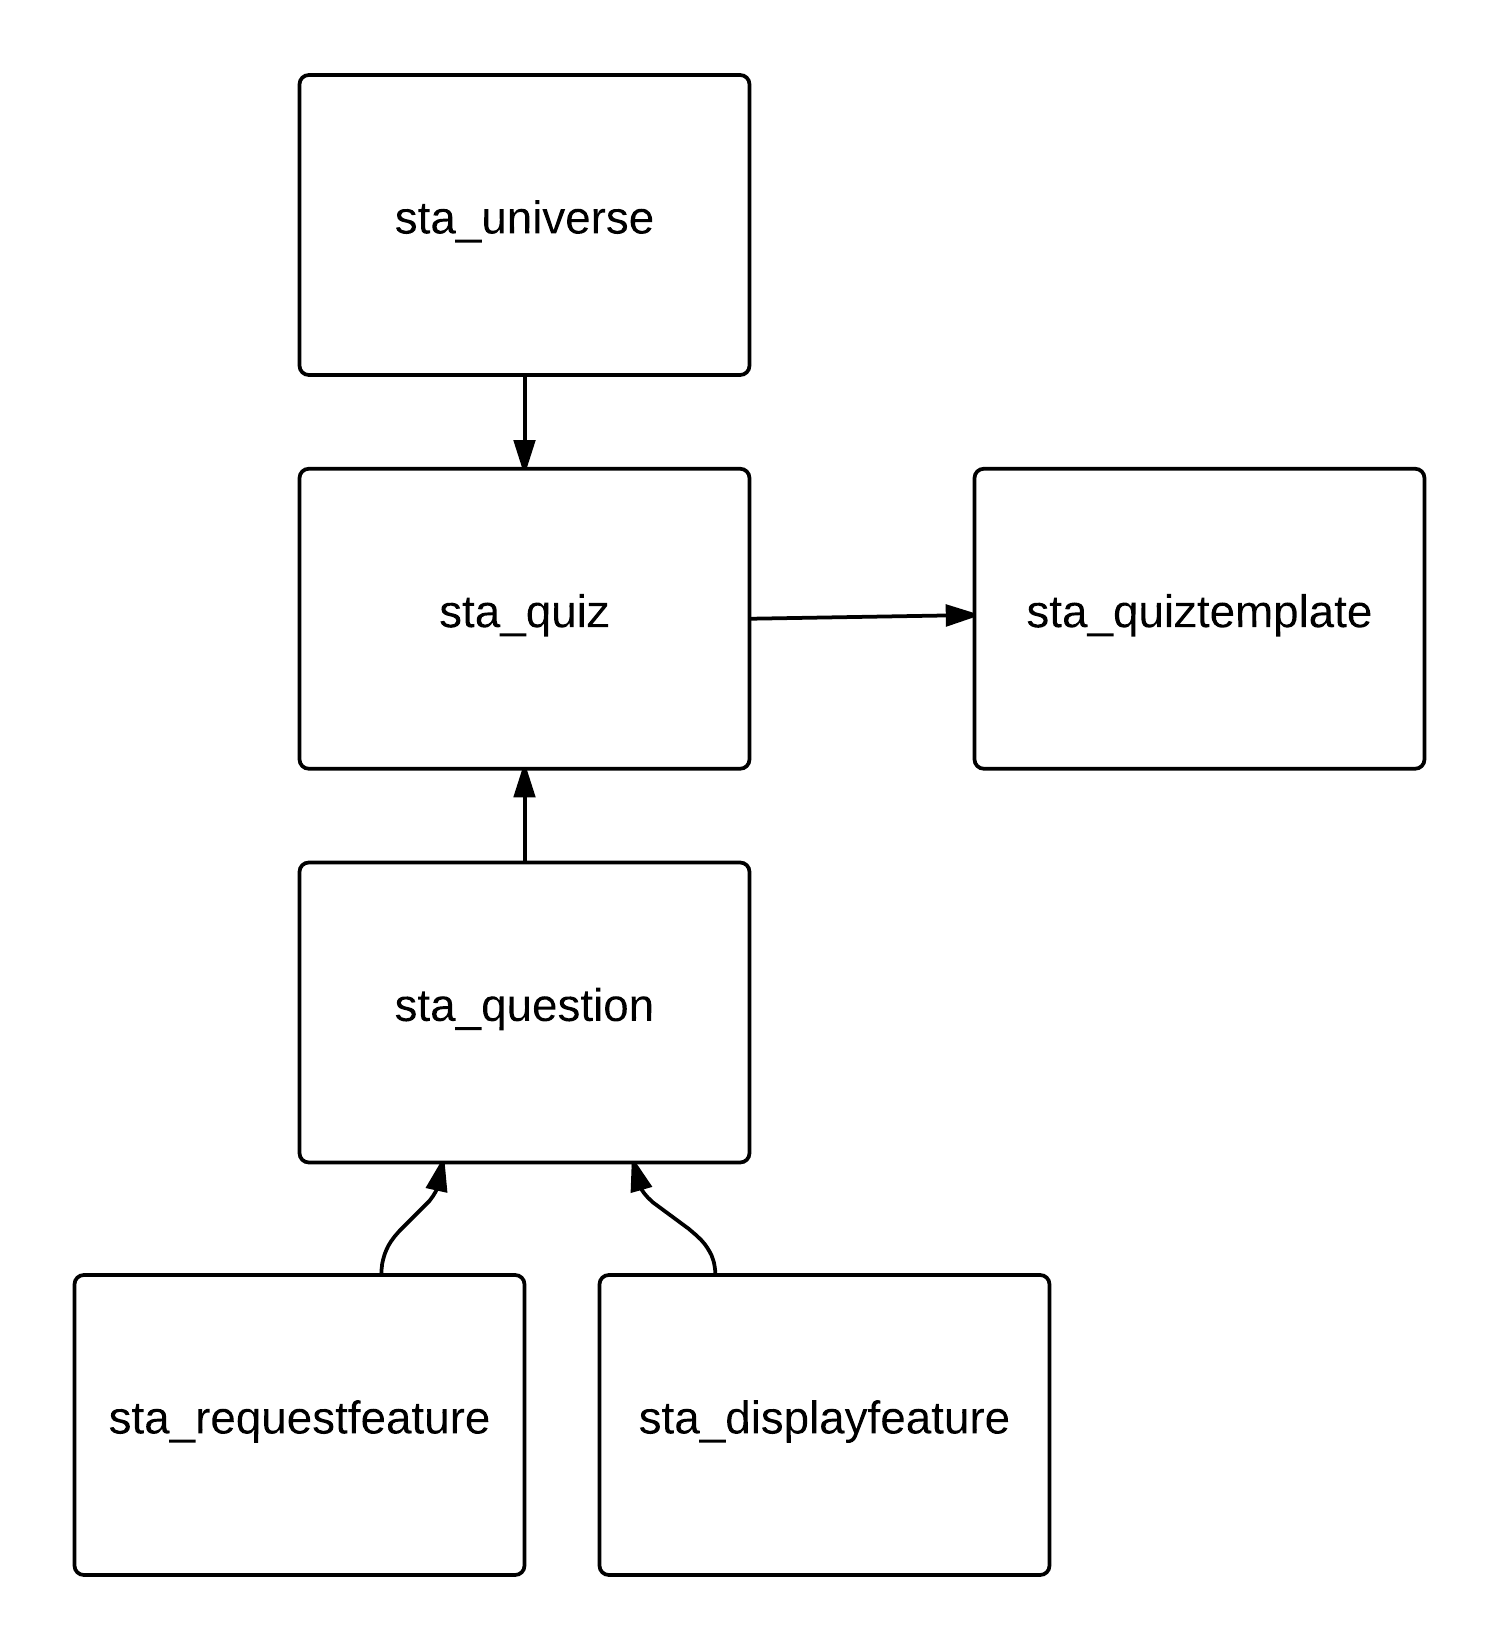
\includegraphics[width=0.7\textwidth]{sta_tables.png}
\end{center}

In this illustration, each arrow indicates a many-to-one relationship, with one item at the arrow
head and many items at the other end of the arrow.


\subsection{The \emph{sta\_quiz} Table}\label{sec-staquiz}\index{sta\_quiz table|hyperit}

Every time a user starts running an exercise, an entry is created in the \emph{sta\_quiz} table. It
contains these fields:

\begin{my-longtabu}{>{\itshape}llX}{ \headiii{\textup{Column}}{Type}{Contents} }
id         & Integer & Unique number identifying this execution of an exercise.\\
userid     & Integer & The \emph{id} field from an entry in the \emph{user} table. This identifies
                       the user running the exercise.\\
templid    & Integer & The \emph{id} field from an entry in the \emph{sta\_quiztemplate} table. This
                       identifies the quiz template used for this exercise.\\
start      & Integer & The start time (UNIX time\footnote{That is, seconds since 00:00:00~UTC on 1~January~1970.}).\\
end        & Integer & The end time (UNIX time). This value is NULL if the exercise is still running or if the
                       exercise was aborted without saving the result.\\
valid      & Boolean & \emph{False} if the user has deleted the entry, \emph{true} otherwise. (There
                        is currently no user interface for deleting statistics.\\
grading    & Boolean & \emph{True} if this entry is to be used for grading
                       purposes, \emph{false} otherwise. (This is controlled by the user clicking
                       ``GRADE task'' or ``SAVE outcome'' at the end of an exercise.) \\
\end{my-longtabu}


\subsection{The \emph{sta\_quiztemplate} Table}\index{sta\_quiztemplate table}

Every time a user starts running an exercise, the system checks if the quiz template%
\index{quiz template}
is already stored in the \emph{sta\_quiztemplate} table. If not, an entry is created. A template is
identified by its contents; if, therefore, a facilitator changes the contents of a quiz template, a
new entry will be created in the \emph{sta\_quiztemplate} table the next time the exercise is run.

The table contains these fields:

\begin{my-longtabu}{>{\itshape}llX}{ \headiii{\textup{Column}}{Type}{Contents} }
id            & Integer  & Unique number identifying this quiz template.\\

userid        & Integer  & The \emph{id} field from an entry in the \emph{user} table. This
                           identifies the user running the exercise. For historical reasons,
                           each user has their own set of templates in this table.\\

pathname      & Text     & The full pathname of the quiz template file.\\

dbname        & Text     & The name of the Emdros database on which the quiz template is based.\\

dbpropname    & Text     & The name of the Grammar Localization Structure for the Emdros database on
                            which the quiz template is based.\\

qoname        & Text     & The Emdros type name of the sentence unit (quiz object) on which the
                           exercise is based.\\

quizcode      & Text     & The actual XML text of the quiz template. Since this text contains both
                           the database name, the name of the Grammar Localization Structure, and the sentence unit,
                           the table fields \emph{dbname, dbpropname,} and \emph{qoname} are
                           actually superfluous, but they are included as separate fields to make
                           decoding the XML text unnecessary in most cases.\\

quizcodehash  & Integer  & A hash value of the \emph{quizcode} field. It can be used to speed up the
                           comparison of the quizcode field from different entries in this table: If
                           the \emph{quizcodehash} values are different, then the \emph{quizcode}
                           values will also be different.\\
\end{my-longtabu}


\subsection{The \emph{sta\_universe} Table}\index{sta\_universe table}

Each entry in the \emph{sta\_universe} table represents a single book, chapter, or verse from the
Bible. Together, a number of entries with the same \emph{quizid} field identify the passages used
for generating a particular exercise.

The \emph{sta\_universe} table contains these fields:

\begin{my-tabu}{>{\itshape}llX}{ \headiii{\textup{Column}}{Type}{Contents} }
id         & Integer & Unique number identifying this entry.\\
userid     & Integer & The \emph{id} field from an entry in the \emph{user} table.\\
quizid     & Integer & The \emph{id} field from an entry in the \emph{sta\_quiz} table.\\
component  & Integer & A reference to a single book, chapter, or verse. The format is either
                       ``Genesis'', ``Genesis:3'', or ``Genesis:3:8''.\\
\end{my-tabu}

\subsection{The \emph{sta\_question} Table}\index{sta\_question table}

Each entry in the \emph{sta\_question} table represents a single question, as defined in Section
\ref{sec-terminology} (see Figure \ref{fig-question} on page \pageref{fig-question}). The table
contains these fields:

\begin{my-tabu}{>{\itshape}llX}{ \headiii{\textup{Column}}{Type}{Contents} }
id         & Integer & Unique number identifying this question.\\
userid     & Integer & The \emph{id} field from an entry in the \emph{user} table.\\
quizid     & Integer & The \emph{id} field from an entry in the \emph{sta\_quiz} table.\\
txt        & Text    & The text of the question. The quiz objects are enclosed
                       between \xml{em} and \xml{/em}.\\
location   & Text    & The Bible reference for the text, given in the format ``Genesis,~3,~8''.\\
time       & Integer & The time (UNIX time) when this question was answered.\\
\end{my-tabu}


\subsection{The \emph{sta\_displayfeature} Table}\index{sta\_displayfeature table}

Each entry in the \emph{sta\_displayfeature} table lists a display feature\index{display feature}
that was shown for a question item\index{question item} (see Section \ref{sec-terminology} and
Figure \ref{fig-question} on page \pageref{fig-question} for a definition of ``question item''.)

The table contains these fields:

\begin{my-tabu}{>{\itshape}llX}{ \headiii{\textup{Column}}{Type}{Contents} }
id         & Integer & Unique number identifying this entry.\\
userid     & Integer & The \emph{id} field from an entry in the \emph{user} table.\\
questid    & Integer & The \emph{id} field from an entry in the \emph{sta\_question} table.\\
qono       & Integer & The index (starting from 1) of the question item within the question.\\
name       & Text    & The name of the feature.\\
value      & Text    & The value of the feature.\\
\end{my-tabu}


\subsection{The \emph{sta\_requestfeature} Table}\index{sta\_requestfeature table}

Each entry in the \emph{sta\_requestfeature} table lists a request feature\index{request feature}
that was required for a question item\index{question item} (see Section \ref{sec-terminology} and
Figure \ref{fig-question} on page \pageref{fig-question} for a definition of ``question item''.)

The table contains these fields:

\begin{my-longtabu}{>{\itshape}llX}{ \headiii{\textup{Column}}{Type}{Contents} }
id         & Integer & Unique number identifying this entry.\\
userid     & Integer & The \emph{id} field from an entry in the \emph{user} table.\\
questid    & Integer & The \emph{id} field from an entry in the \emph{sta\_question} table.\\
qono       & Integer & The index (starting from 1) of the question item within the question.\\
name       & Text    & The name of the feature.\\
value      & Text    & The correct value of the feature.\\
answer     & Text    & The answer provided by the user. If the user tries to answer several times in
                       a single exercise, only the first answer is recorded.\\
correct    & Boolean & \emph{True} if the user's answer is correct.\footnote{This is not the same as
  testing if \emph{value}=\emph{answer}. For example, when providing an English translation of a
  word, a correct \emph{answer} may be ``do'' even if the \emph{value} is ``make, do; fix; deal with''.}\\
\end{my-longtabu}

%%%%%%%%%%%%%%%%%%%% The heb_urls Table %%%%%%%%%%%%%%%%%%%%
\section{The \emph{heb\_urls} Table}%
\index{heb\_urls table}

The \emph{heb\_urls} table keeps track of the hyperlinks associated with Hebrew or Aramaic lexemes.

The table contains these fields:

\begin{my-longtabu}{>{\itshape}llX}{ \headiii{\textup{Column}}{Type}{Contents} }
id       & Integer & Unique number identifying this entry.\\
lex      & Text    & The value of the \emph{lex} feature from the ETCBC4 database.\\
language & Text    & The value of the \emph{language} feature from the ETCBC4 database.\\
url      & Text    & The URL that is the destination of the hyperlink.\\
icon     & Text    & The name of an icon to use for this hyperlnk. The valid icon names can be found
in the file \texttt{myapp/helpers/icon\_helper.php}.\\
\end{my-longtabu}


%%%%%%%%%%%%%%%%%%%% The migrations Table %%%%%%%%%%%%%%%%%%%%
\section{The \emph{migrations} Table}%
\index{migrations table}

The \emph{migrations} table is maintained by the migration mechanism of CodeIgniter. This mechanism
keeps track of system updates. It contains this field:

\begin{my-tabu}{>{\itshape}lll}{ \headiii{\textup{Column}}{Type}{Contents} }
version & Integer & Current system version number as used by CodeIgniter.\\
\end{my-tabu}



%%%%%%%%%%%%%%%%%%%% The Localization Tables %%%%%%%%%%%%%%%%%%%%

\section{The Localization Tables}\label{sec-localization-tables}\index{localization}

The \emph{translation\_languages} table plus the tables with names starting with \emph{db\_localize},
\emph{language\_} or \emph{lexicon\_} contain information for the localization of text.

\subsection{The \emph{translation\_languages} Table}\label{sec-translation-languages}\index{translation\_languages table}

The \emph{translation\_languages} table contains information about available translations of the
user interface and the lexicons. It contains one entry per localization language.

The table contains these fields:

\begin{my-longtabu}{>{\itshape}llX}{ \headiii{\textup{Column}}{Type}{Contents} }
  id     & Integer & Unique number identifying this entry.     \\
  abb    & Text    & ISO~639-1 language code.                  \\
  internal & Text & The internal name of the language. This is typically the uncapitalized english
  name of the
  language; for example, ``german'' for German.                  \\
  native & Text & The name of the language in the language itself; for example, ``Deutsch'' for German. \\
  iface\_enabled & Boolean & \emph{True} if a translation of the Bible OL user interface and the
  grammar information exists in the localization language. \\
  heblex\_enabled & Boolean & \emph{True} if a translation of the Hebrew and Aramaic lexicons exists in the localization language. \\
  greeklex\_enabled & Boolean & \emph{True} if a translation of the Greek lexicons exists in the localization language. \\
\end{my-longtabu}


\subsection{The \emph{db\_localize} and \emph{db\_localize\_VARIANT} Tables}\label{sec-db-localize}\index{db\_localize table|hyperit}\index{db\_localize\_VARIANT table|hyperit}

The \emph{db\_localize} table and the optional \emph{db\_localize\_VARIANT} tables contain the
Grammar Localization Structures\index{Grammar Localization Structure}, that is, the translation of
grammar terms into various languages. For details, see Section \ref{sec-gram-loc-struct}.

The tables contain these fields:

\begin{my-longtabu}{>{\itshape}llX}{ \headiii{\textup{Column}}{Type}{Contents} }
id     & Integer & Unique number identifying this entry.     \\
db     & Text    & The name of the Grammar Localization Structure. \\
lang   & Text    & The language code code for the translation (``en'' for English, ``da''
                   for Danish, etc.). The special value ``comment'' is used for an entry
                   providing context and formatting information used in the tranlator's interface
                   (see Section \ref{sec-gram-loc-comments}). \\
json   & Text    & A JSON string containing the Grammar Localization Structure. \\
\end{my-longtabu}

If a variant is not active (see Section \ref{sec-variants}), the system only consults the
\emph{db\_localize} table. If a variant is active and a corresponding entry exists in the relevant
\emph{db\_localize\_VARIANT} table, that entry will be used instead of the entry in the
\emph{db\_localize} table.


\subsection{The \emph{language\_comment} Table}\label{sec-language-comment}\index{language\_comment
  table|hyperit}

The \emph{language\_comment} table contains information describing the available translation strings
for the user interface. This table is used by the translator's interface. Each
\emph{textgroup}/\emph{symbolic\_name} pair in this table matches an entry in each
\emph{language\_LANG} table.

The table contains these fields:

\begin{my-longtabu}{>{\itshape}llX}{ \headiii{\textup{Column}}{Type}{Contents} }
id             & Integer & Unique number identifying this entry.     \\
textgroup      & Text    & See Section \ref{sec-loc-user-interface}. \\
symbolic\_name & Text    & See Section \ref{sec-loc-user-interface}. \\
comment        & Text    & A string providing the human translator with context for when the string is used. \\
format         & Text    & If this value is ``keep\_blanks'', whitespace characters in the string
                           are important. If the value is \emph{NULL}, multiple contiguous
                           whitespace characters are replaced by a single space. \\
use\_textarea  & Boolean & \emph{True} if the translator's interface should use a
                           \xml{textarea} HTML element for input. \emph{False} if an
                           \xml{input type="text"} HTML element should be used.\\
\end{my-longtabu}


\subsection{The \emph{language\_LANG} and \emph{language\_LANG\_VARIANT} Tables}\label{sec-language-lang}\index{language\_LANG table|hyperit}\index{language\_LANG\_VARIANT table|hyperit}

The system contains a number of tables with names such as \emph{language\_en} for English,
\emph{language\_da} for Danish, etc. Additionally variant tables for each language may exist. The
tables provide translations of the user interface.

The tables contain these fields:

\begin{my-longtabu}{>{\itshape}llX}{ \headiii{\textup{Column}}{Type}{Contents} }
id             & Integer & Unique number identifying this entry.     \\
textgroup      & Text    & See Section \ref{sec-loc-user-interface}. \\
symbolic\_name & Text    & See Section \ref{sec-loc-user-interface}. \\
text           & Text    & The relevant string translated into language \emph{LANG}. \\
\end{my-longtabu}

If a variant is not active (see Section \ref{sec-variants}), the system only consults the
\emph{language\_LANG} table. If a variant is active and a corresponding entry exists in the relevant
\emph{language\_LANG\_VARIANT} table, that entry will be used instead of the entry in the
\emph{language\_LANG} table.



\subsection{The \emph{lexicon\_Hebrew} and \emph{lexicon\_Aramaic} Tables}\label{sec-lexicon-heb}%
\index{lexicon\_Hebrew table|hyperit}\index{lexicon\_Aramaic table|hyperit}

The \emph{lexicon\_Hebrew} table contains information about all the Hebrew lexemes used by
the system. Similarly, the \emph{lexicon\_Aramaic} table contains information about all the Aramaic lexemes.

The tables contain these fields:

\begin{my-longtabu}{>{\itshape}llX}{ \headiii{\textup{Column}}{Type}{Contents} }
id                      & Integer & Unique number identifying this entry.     \\
lex                     & Text    & The lexeme in the \emph{transcribed alphabet} (see page \pageref{page-transcribed}). \\
vs                      & Text    & The verbal stem of the word. ``NA'' if the word is not a verb. \\
tally                   & Integer & The number of occurrences of this word in the text. \\
vocalized\_lexeme\_utf8 & Text    & The lexeme in Hebrew characters. \\
roman                   & Text    & An optional roman numeral to differentiate between identically spelled lexemes.\\
sortorder               & Text    & A string that can be used to sort the words alphabetically. \\
firstbook               & Text    & \multirow{3}{\linewidth}{The book, chapter, and verse of the first occurrence of the word.} \\
firstchapter            & Integer & \\
firstverse              & Integer & \\
\end{my-longtabu}

An entry is uniquely defined by its \emph{lex} and \emph{vs} fields.

\subsection{The \emph{lexicon\_Hebrew\_LANG}, \emph{lexicon\_Aramaic\_LANG},
  \emph{lexicon\_Hebrew\_LANG\_VARIANT}, and \emph{lexicon\_Aramaic\_LANG\_VARIANT} Tables}\label{sec-lexicon-heb-lang}%
\index{lexicon\_Hebrew\_LANG table|hyperit}\index{lexicon\_Aramaic\_LANG table|hyperit}%
\index{lexicon\_Hebrew\_LANG\_VARIANT table|hyperit}\index{lexicon\_Aramaic\_LANG\_VARIANT table|hyperit}

The system contains a number of tables with names such as \emph{lexicon\_Hebrew\_en} for English and
\emph{lexicon\_Hebrew\_de} for German. They provide translations for the lexemes listed in the
\emph{lexicon\_Hebrew} table. Similar tables, such as \emph{lexicon\_Aramaic\_en,} provide
translations for the lexemes listed in the \emph{lexicon\_Aramaic} table. Additionally variant
tables for each language may exist.

The tables contain these fields:

\begin{my-longtabu}{>{\itshape}llX}{ \headiii{\textup{Column}}{Type}{Contents} }
id      & Integer & Unique number identifying this entry. \\
lex\_id & Integer & The \emph{id} field of the entry in the \emph{lexicon\_Hebrew} or
                    \emph{lexicon\_Aramaic} table for which the current entry provides a translation. \\
gloss   & Text    & The translation of the lexeme into language \emph{LANG}. \\
\end{my-longtabu}


If a variant is not active (see Section \ref{sec-variants}), the system only consults the
\emph{lexicon\_\ldots\_LANG} table. If a variant is active and a corresponding entry exists in the relevant
\emph{lexicon\_\ldots\_LANG\_VARIANT} table, that entry will be used instead of the entry in the
\emph{lexicon\_\ldots\_LANG} table.


\subsection{The \emph{lexicon\_greek} Table}\label{sec-lexicon-greek}\index{lexicon\_greek table|hyperit}

The \emph{lexicon\_greek} table contains information about all the Greek lexemes used by
the system.

The tables contain these fields:

\begin{my-longtabu}{>{\itshape}llX}{ \headiii{\textup{Column}}{Type}{Contents} }
id                  & Integer & Unique number identifying this entry.     \\
strongs             & Integer & The Strong's number for the lexeme. \\
strongs\_unreliable & Boolean & \emph{True} if the indicated Strong's number is considered unreliable.\\
lemma               & Text    & The lexeme in accented Greek characters.\\
tally               & Integer & The number of occurrences of this word in the text. \\
sortorder           & Text    & The lexeme in unaccented, lowercase Greek characters, which can be
                                used to sort the words alphabetically. \\
firstbook           & Text    & \multirow{3}{\linewidth}{The book, chapter, and verse of the first occurrence of the word.} \\
firstchapter        & Integer & \\
firstverse          & Integer & \\
\end{my-longtabu}


\subsection{The \emph{lexicon\_greek\_LANG} and \emph{lexicon\_greek\_LANG\_VARIANT }Tables}\label{sec-lexicon-greek-lang}\index{lexicon\_greek\_LANG table|hyperit}\index{lexicon\_greek\_LANG\_VARIANT table|hyperit}

The system contains a number of tables with names such as \emph{lexicon\_greek\_en} for English.
They provide translations for the lexemes listed in the \emph{lexicon\_greek} table. Additionally variant
tables for each language may exist.

The tables contain these fields:

\begin{my-longtabu}{>{\itshape}llX}{ \headiii{\textup{Column}}{Type}{Contents} }
id      & Integer & Unique number identifying this entry. \\
lex\_id & Integer & The \emph{id} field of the entry in the \emph{lexicon\_greek} table for
                    which the current entry provides a translation. \\
gloss   & Text    & The translation of the lexeme into language \emph{LANG}. \\
\end{my-longtabu}

If a variant is not active (see Section \ref{sec-variants}), the system only consults the
\emph{lexicon\_greek\_LANG} table. If a variant is active and a corresponding entry exists in the relevant
\emph{lexicon\_greek\_LANG\_VARIANT} table, that entry will be used instead of the entry in the
\emph{lexicon\_greek\_LANG} table.



%%%%%%%%%%%%%%%%%%%%%%%%%%%%%%%%%%%%%%%%%%%%%%%%%%%%%%%%%%%
%%%%%%%%%%%%%%%%%%%% Less Style Sheets %%%%%%%%%%%%%%%%%%%%
\chapter{Less Style Sheets}\label{chap-less-use}\index{Less|hyperit}

\textbf{Read this chapter if you are going to understand or modify style sheets.}
\plainbreak{3}

CSS\index{CSS} style sheets can sometimes be unwieldy to work with. The \emph{Less} program is a CSS
preprocessor that allows a clearer way to structure style sheets.

Compare, for example, the CSS code in the left column below with the Less code in the right column:

\lstset{frame=} % Cannot set in a lstlisting inside tabular

\begin{center}
\begin{tabular}{p{0.45\textwidth}p{0.45\textwidth}}
\hline
\textbf{CSS} & \textbf{Less}\\
\hline
\begin{lstlisting}[language=CSS,aboveskip=0mm,belowskip=0mm]



|ul.dropdown| {
  /padding/: 0;
}

|ul.dropdown a| {
  /text-decoration/: none;
}

|ul.dropdown li| {
  /display/: inline-block;
  /background/: #f3d673;
  /z-index/: 1;
}

|ul.dropdown li:hover| {
  /background/: #c0c0c0;
  /position/: relative;
}

|ul.dropdown li a| {
  /color/: black;
  /display/: block;
}
\end{lstlisting}

&

\begin{lstlisting}[language=CSS,aboveskip=0mm,belowskip=0mm]
@beige: #f3d673;
@mediumgray: #c0c0c0;

|ul.dropdown| {
    /padding/: 0;

    |a| {
        /text-decoration/: none;
    }

    |li| {
        /display/: inline-block;
        /background/: @beige;
        /z-index/: 1;

        |&:hover| {
            /background/: @mediumgray;
            /position/: relative;
        }

        |a| {
            /color/: black;
            /display/: block;
        }
    }
}
\end{lstlisting}\\
\hline
\end{tabular}
\end{center}


\lstset{frame=tb} % Restore value set above


Section \ref{sec-installing-lessc} describes how to install the Less compiler
\emph{lessc}\index{lessc}. Details of the Less language can be found at \url{http://lesscss.org}.

Although Less style files can be compiled when used in a browser, the Bible OL implementation
compiles Less files only once and stores the resulting CSS files. This is achieved through the
Makefile\index{Makefile} in the top directory. The command ``make\index{make} styles/ol.css'' will compile the Less
file.\footnote{The simple command ``make'' will compile all Less and TypeScript files.}

At present, Bible OL uses only one Less file, namely \texttt{styles/ol.less} which compiles into
\texttt{styles/ol.css}.

%%%%%%%%%%%%%%%%%%%%%%%%%%%%%%%%%%%%%%%%%%%%%%%%%%%%%
%%%%%%%%%%%%%%%%%%%% Client Code %%%%%%%%%%%%%%%%%%%%
\chapter{Client Code}\label{chap-client-code}\index{client}

\textbf{Read this chapter if you are going to understand or modify the client code.}
\plainbreak{3}

The client code runs in a web browser. Most of it is written in TypeScript which is compiled into
JavaScript\index{JavaScript}.

There are three different TypeScript programs that can run as client code:


\begin{itemize}
\item \emph{ol,}\index{ol (TypeScript program)} which displays text or runs exercises. (See Section \ref{sec-ol}.)
\item \emph{editquiz,} which edits a quiz template.
\item \emph{fontselector,} which allows a user to set font preferences.
\end{itemize}

%%%%%%%%%%%%%%%%%%%% TypeScript %%%%%%%%%%%%%%%%%%%%
\section{TypeScript}\label{sec-typescript-use}\index{TypeScript|hyperit}

TypeScript is a superset of JavaScript that adds strong typing and proper classes to JavaScript.\index{JavaScript}
The website \url{http://www.typescriptlang.org} contains a tutorial and the formal specification of
the language.

Section \ref{sec-installing-tsc} describes how to install the TypeScript compiler \emph{tsc}.\index{tsc}

The Bible OL implementation compiles TypeScript files only once and stores the resulting JavaScript
files. This is achieved through the Makefile\index{Makefile} in the top directory. The command ``make all'' (or
simply ``make'')\index{make} will compile the TypeScript files (and the Less file).

The TypeScript files are found in the directory \texttt{ts}; the resulting JavaScript files are
stored in the directory \texttt{js}.

%%%%%%%%%%%%%%%%%%%% The ol Client Code %%%%%%%%%%%%%%%%%%%%
\section{The \emph{ol} Client Code}\label{sec-ol}\index{ol (TypeScript program)|hyperit}

The \emph{ol} client code is responsible for displaying text and running an exercise based on
information provided by the server -- primarily in the JavaScript variables \emph{configuration,}%
\index{configuration JavaScript variable@\emph{configuration} JavaScript variable}
\emph{l10n,}%
\index{l10n JavaScript variable@\emph{l10n} JavaScript variable}
\emph{l10n\_js,}%
\index{l10n_js JavaScript variable@\emph{l10n\_js} JavaScript variable}
\emph{typeinfo,}%
\index{typeinfo JavaScript variable@\emph{typeinfo} JavaScript variable}
\emph{dictionaries,}%
\index{dictionaries JavaScript variable@\emph{dictionaries} JavaScript variable}
and \emph{quizdata,}%
\index{quizdata JavaScript variable@\emph{quizdata} JavaScript variable}
which are described in detail in Chapters \ref{chap-data-exchange} and \ref{chap-dictionary}.

For text display, the \emph{ol} program builds the text inside an HTML\index{HTML} skeleton provided by the
server. The skeleton looks like this (somewhat simplified):


\begin{lstlisting}[language=HTML]
<div class="grammarselector" id="gramselect"></div>
<div class="grammardisplay"></div>

<div id="textcontainer">
    <h1></h1>
    <div id="textarea"></div>
    <p><button id="togglemql">Toggle MQL</button></p>
    <pre class="mqlarea">SELECT ALL OBJECTS WHERE ...</pre>
</div>
\end{lstlisting}

When running an exercise, the \emph{ol} program builds a question inside an HTML skeleton provided by the
server. The skeleton looks like this (somewhat simplified):

\begin{lstlisting}[language=HTML,morekeywords={progress}]
<div class="grammarselector" id="gramselect"></div>
<div class="grammardisplay"></div>
 
<div id="textcontainer">
    <div id="quizdesc"></div>
    <div id="textarea"></div>
    <div id="virtualkbcontainer"><div id="virtualkbid"></div></div>
    <table id="quiztab"></table>
    <p><input id="locate_cb" type="checkbox">Locate: <span class="location"></span></p>

    <p class="inline">Progress:</p>
    <progress id="progress" value="0" max="1"></progress>
    <div id="progressbar"></div>
    <p id="progresstext" class="inline"></p>

    <div id="buttonlist1">
        <button id="check_answer" type="button">Check answer</button>
        <button id="show_answer" type="button">Show answer</button>
    </div>
    <div id="buttonlist2">
        <button id="next_question" type="button">Next</button>
        <button id="finish" type="button">GRADE task</button>
        <button id="finishNoStats" type="button">SAVE outcome</button>
    </div>

    <p><button id="togglemql">Toggle MQL</button></p>
    <pre class="mqlarea">SELECT ALL OBJECTS WHERE ...</pre>
</div>
\end{lstlisting}
  
The \xml{div class="grammarselector"} element is for the grammar selection box%
\index{grammar selection box}.
The \emph{ol} program generates the contents of this element using the class
\emph{GenerateCheckboxes}.

The \xml{div class="grammardisplay"} element is for the grammar information box.%
\index{grammar information box}
It is built by the function \emph{toolTipFunc,} which is defined within the function
\emph{generateSentenceHtml} in the \emph{Dictionary} class.

The \xml{div class="textcontainer"} element contains the text and, possibly, the question. The
actual text is placed in the \xml{div class="textarea"} element. The question items are placed
in the \xml{table id="quiztab"} table.

The \xml{button id="togglemql"} button and the \xml{pre class="mqlarea"} element are normally not
shown to the user. They are intended for debugging only. The \xml{pre class="mqlarea"} element
contains the MQL\index{MQL!displaying in web page} commands executed during the creation of the text
or exercise. You can either inspect the element by looking at the HTML source sent to the browser,
or you can enable the \xml{button id="togglemql"} button by removing ``\texttt{display:~none}'' from
this instruction in \texttt{styles/ol.less}:\footnote{After modifying \texttt{styles/ol.less}, you
  must recompile the Less file. For simple debugging, you may prefer to edit the
  \texttt{styles/ol.css} file directly.}

\begin{lstlisting}[language=CSS,frame=]
|button#togglemql| {
    /display/: none;
}
\end{lstlisting}

When the ``\texttt{display:~none}'' line has been removed, a ``Toggle MQL'' button will appear in
the browser. Clicking the button will display the MQL commands executed during the creation of the
text or exercise.

\pfbreak

The most complicated task for \emph{ol} is probably to build the contents of the \emph{textarea},
and this will be described in some detail below.

As Chapter \ref{chap-dictionary} explains, the \emph{dictionaries} variable contains the field
\emph{sentenceSets,} which is an array of \emph{MonadSet}%
\index{MonadSet TypeScript interface@\emph{MonadSet} TypeScript interface}
objects, and the field \emph{monadObjects,} which is an array of arrays of arrays of
\emph{MonadObject}%
\index{MonadObject TypeScript interface@\emph{MonadObject} TypeScript interface}
objects. When Bible OL is displaying text, the array \emph{sentenceSets} and the top array in
\emph{monadObjects} have only one element; but when Bible OL is displaying an exercise consisting of
\emph{n} questions, the two arrays have \emph{n} elements.

The \emph{ol} program converts the \emph{dictionaries}%
\index{dictionaries JavaScript variable@\emph{dictionaries} JavaScript variable}
variable (which is of interface class \emph{DictionaryIf})%
\index{DictionaryIf TypeScript interface@\emph{DictionaryIf} TypeScript interface}
into one or more objects of class \emph{Dictionary},%
\index{Dictionary TypeScript class@\emph{Dictionary} TypeScript class}
one for each entry in the \emph{MonadSets/MonadObject} arrays. (Note the \emph{Dictionary} class
here must not be confused with the \emph{Dictionary} class in the server. The server's
\emph{Dictionary} class corresponds to the client's \emph{DictionaryIf} interface.)

As explained in Section \ref{sec-dictionaryif}, the \emph{monadObjects} field of the
\emph{DictionaryIf} interface is an array of array of arrays. The middle array is indexed by the
level in the grammatical hierarchy\index{grammar hierarchy} (word, phrase, clause, etc.). As part of
creating a \emph{Dictionary} from a given index in a \emph{DictionaryIf}, the \emph{constructor}
function in the \emph{Dictionary} class builds a parallel collection of arrays: Each
\emph{MonadObjects} is complemented by one or more \emph{DisplayMonadObjects}.%
\index{DisplayMonadObject TypeScript class@\emph{DisplayMonadObject} TypeScript class}
A \emph{DisplayMonadObject} represents the physical appearance of an Emdros object in the browser.
\emph{DisplayMonadObject} has a member function, \emph{generateHtml,} which is responsible for
generating the HTML that renders the Emdros object.

Just as a \emph{MonadObject} is either a \emph{SingleMonadObject}%
\index{SingleMonadObject TypeScript interface@\emph{SingleMonadObject} TypeScript interface}
or a \emph{MultipleMonadObject},%
\index{MultipleMonadObject TypeScript interface@\emph{MultipleMonadObject} TypeScript interface}
a \emph{DisplayMonadObject} is either a \emph{DisplaySingleMonadObject}%
\index{DisplaySingleMonadObject TypeScript class@\emph{DisplaySingleMonadObject} TypeScript class}
(typically representing a word) or a \emph{DisplayMultipleMonadObject}%
\index{DisplayMultipleMonadObject TypeScript class@\emph{DisplayMultipleMonadObject} TypeScript class}
(typically representing a phrase, clause, or sentence).
There is, however, an important difference between a \emph{MultipleMonadObject} and a
\emph{DisplayMultipleMonadObject}. If, for example, a clause consists of multiple noncontiguous
parts, it is represented by one \emph{MultipleMonadObject} but by multiple
\emph{DisplayMultipleMonadObjects,} one for each part of the clause.

When the \emph{generateHtml} is called for a \emph{DisplaySingleMonadObject,} its task is to create
HTML code to represent a single word and all its features. The code generated is structured as shown
in Listing \ref{list-html-word}.

\begin{lstlisting}[language=HTML,caption=HTML display structure for a word object,label=list-html-word]
<span class="textblock inline">
    <span class="textdisplay %\textrm{\textit{charset}}%" %{\color{blue} data-idd}%="%\textrm{\textit{ID\_D}}%">%\textrm{\textit{text}}%</span>

    <span class="wordgrammar dontshowit %\textrm{\textit{featurename}}% %\textrm{\textit{charset}}%">%\textrm{\textit{featurevalue}}%</span>
    <span class="wordgrammar dontshowit %\textrm{\textit{featurename}}% %\textrm{\textit{charset}}%">%\textrm{\textit{featurevalue}}%</span>
    <span class="wordgrammar dontshowit %\textrm{\textit{featurename}}% %\textrm{\textit{charset}}%">%\textrm{\textit{featurevalue}}%</span>
    ...
  
</span>
\end{lstlisting}


\begin{minipage}{\textwidth}
Here,

\begin{tabu}{>{\itshape}lX}
charset & identifies the character set and hence the font and text direction. Valid values are
          \xmla{hebrew}, \xmla{hebrew\_translit}, \xmla{greek}, \xmla{latin}, and \xmla{ltr}. The
          value \xmla{ltr} is used to force left-to-right for features in Latin script. The value
          \xmla{latin} is currently not used; it is reserved for corpuses that use the Latin
          alphabet.\\

ID\_D & is the ID\_D\index{Emdros!ID\_D} (see Chapter \ref{chap-emdros-use}) of the word.\\

text & is the actual word.\\

featurename & is the non-localized name of the feature, that is, the name of the feature as it
appears in the Emdros database.\\

featurevalue & is the localized value of the feature.\\
\end{tabu}
\end{minipage}

If a particular feature is turned on in the grammar selection box\index{grammar selection box}, the
\xmla{dontshowit} class in the relevant \xml{span} elements is changed to \xmla{showit.}

Two extra class values are added to the \xml{span class="textdisplay"} element to control the
rendering of Hebrew word spacing.\index{space (between words)}

The first class value is one of these and doesn't change:

\begin{my-tabu}{>{\ttfamily}lX}{ \headii{\textrm{Class value}}{Meaning} }
  cont & The word must be followed immediately by the next word with no intervening space.\\

  contx & The word ends in a \emph{maqaf}\index{maqaf} (\heb{־}) and must be followed immediately by the next word
  with no intervening space.\\
\end{my-tabu}

If neither \xmla{cont} nor \xmla{contx} is set on a word, a \xml{span} element with class
\xmla{wordspace} is inserted after the word.


The second class value is one of these, and it changes as the user switches between display and not
displaying word spacing:

\begin{my-tabu}{>{\ttfamily}lX}{ \headii{\textrm{Class value}}{Meaning} }
  cont1 & The user has not requested word spacing. Use default rending of words.\\

  cont2 & The user has requested word spacing. Add a hyphen and a space to the end of the current
          word.\\

  cont2x & The user has requested word spacing. The current word ends in a
           \emph{maqaf}\index{maqaf}. Add a space to the end of the current word.\\
\end{my-tabu}

When the \emph{generateHtml} is called for a \emph{DisplayMultipleMonadObject,}%
\index{DisplayMultipleMonadObject TypeScript class@\emph{DisplayMultipleMonadObject} TypeScript class}
its task is to create HTML code to represent a phrase, clause, or sentence object and all its
features. The code generated is structured as shown in Listing \ref{list-html-clause}.

\begin{lstlisting}[language=HTML,caption=HTML display structure for a phrase/clause/sentence object,label=list-html-clause]
<span class="notdummy %\textrm{\textit{nolevel}}% noseplin">
    <span class="gram dontshowit" %{\color{blue}data-idd}%="%\textrm{\textit{ID\_D}}%">%\textrm{\textit{loctype}}%
         <span class="xgrammar dontshowit %\textrm{\textit{type}}%_%\textrm{\textit{featurename}}%">:%\textrm{\textit{featurevalue}}%</span>
         <span class="xgrammar dontshowit %\textrm{\textit{type}}%_%\textrm{\textit{featurename}}%">:%\textrm{\textit{featurevalue}}%</span>
         <span class="xgrammar dontshowit %\textrm{\textit{type}}%_%\textrm{\textit{featurename}}%">:%\textrm{\textit{featurevalue}}%</span>
         ....
    </span>
    ... %\textrm{\scriptsize(Lower levels in the grammar hierarchy are inserted here)}%
</span>
\end{lstlisting}

\begin{minipage}{\textwidth}
Here,

\begin{tabu}{>{\itshape}lX}
nolevel & is one of \xmla{nolev1}, \xmla{nolev2}, \xmla{nolev3}, etc. The number within this
          name identifies the level in the grammar hierarchy: 1 for the level just above
          \emph{word}, 2 for the next higher level, etc.\\

ID\_D & is the ID\_D\index{Emdros!ID\_D} (see Chapter \ref{chap-emdros-use}) of the word.\\

loctype & is the localized name of the Emdros object type.\\

type & is the non-localized name of the Emdros object type, that is, the name of the type as it
appears in the Emdros database.\\

featurename & is the non-localized name of the feature, that is, the name of the feature as it
appears in the Emdros database. Note that \emph{type} and \emph{featurename} are strung together
with an intervening underscore, thus forming a single class value.\\

featurevalue & is the localized value of the feature.\\
\end{tabu}
\end{minipage}

The \xml{span class="notdummy"} element may additionally have the class value \xmla{hasp}
and/or \xmla{hass}. This indicates that the current \emph{DisplayMultipleMonadObject} is part of a
noncontiguous collection of monads. The class value \xmla{hasp} means that the
\emph{DisplayMultipleMonadObject} has a predecessor; the class value \xmla{hass} means that the
\emph{DisplayMultipleMonadObject} has a successor.


If ``Show border'' is selected in the grammar selection box\index{grammar selection box} for a
particular level in the grammar hierarchy, the \xmla{dontshowit} class in the relevant \xml{span
  class="gram"} elements is changed to \xmla{showit.}

If ``Separate lines'' is selected in the grammar selection box\index{grammar selection box} for a
particular level in the grammar hierarchy, the \xmla{noseplin} class in the relevant \xml{span
  class="notdummy"} elements is changed to \xmla{seplin.}

If a particular feature is turned on in the grammar selection box\index{grammar selection box}, the
\xmla{dontshowit} class in the relevant \xml{span class="xgrammar"} elements is changed to
\xmla{showit.}


Occasionally\footnote{Currently only in the nestle1904 database.}, a level in the grammar hierarchy
is missing. If this is the case, the server code will insert a dummy object\index{dummy object} in
the hierarchy, and the client will generated this HTML code:

\begin{lstlisting}[language=HTML]
<span class="%\textrm{\textit{nolevel}}% noseplin">
    <span class="nogram dontshowit" %{\color{blue}data-idd}%="%\textrm{\textit{ID\_D}}%">%\textrm{\textit{loctype}}%
    </span>
    ... %\textrm{\scriptsize(Lower levels in the grammar hierarchy are inserted here)}%
</span>
\end{lstlisting}

Note the absence of the \xmla{notdummy} class value.


At the top (patriarch\index{patriarch}) level the \xmla{notdummy} class name is omitted, and at this
level the HTML simply looks like this:

\begin{lstlisting}[language=HTML]
<span class="%\textrm{\textit{nolevel}}% noseplin">
    ... %\textrm{\scriptsize(Lower levels in the grammar hierarchy are inserted here)}%
</span>
\end{lstlisting}

%%%%%%%%%%%%%%%%%%%% The editquiz Client Code %%%%%%%%%%%%%%%%%%%%
\section{The \emph{editquiz} Client Code}\label{sec-editquiz}\index{editquiz (TypeScript
  program)|hyperit}

The \emph{editquiz} client code is not described in detail here. Its purpose is to allow users to
edit a quiz template. There is, however, one feature that requires some explanation: The ability to
import queries from SHEBANQ.

\subsection{Import from SHEBANQ}\label{sec-shebanq-import}\index{SHEBANQ}

The SHEBANQ website (see Section \ref{sec-shebanq}) allows its users to create MQL queries using the
ETCBC4 Hebrew database. Such queries can be imported into Bible OL.

First, the user must identify the query ID at the SHEBANQ website. The number is found in the
upper left corner of a query page at SHEBANQ:

\begin{center}
  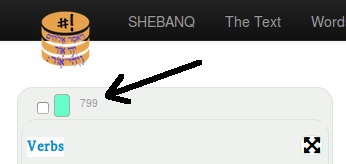
\includegraphics[width=0.5\textwidth]{shebanq.png}
\end{center}

In this example, the query ID is 799.

When editing a quiz template on Bible OL, a user can request the client code to import this query
from SHEBANQ.

The \emph{editquiz} client code sends a request to the \emph{import\_shebanq} function in the
\emph{ctrl\_shebanq} controller. This in turn sends a request to
\url{https://shebanq.ancient-data.org/hebrew/query.json?id=799} which returns a JSON representation
of the MQL query.


%%%%%%%%%%%%%%%%%%%%%%%%%%%%%%%%%%%%%%%%%%%%%%%%%%%%%%
%%%%%%%%%%%%%%%%%%%% Localization %%%%%%%%%%%%%%%%%%%%
\chapter{Internationalization and Localization}\label{chap-localize}\index{localization}\index{internationalization}

\textbf{As a developer, you must read this chapter.}

\plainbreak{3}

\section{CodeIgniter's Internationalization Mechanism}

CodeIgniter provides a mechanism for developing internationalized software. The basic rule is never
to write English text directly in the code. All text strings must be given a name, and a
language-specific version of that text is stored in an array called \emph{\$lang}.

The language specific strings are located in the directory \texttt{myapp/language}. This directory
has a subdirectory for each supported language. The name of the subdirectory is the international
two-letter abbreviation of the language as specified in the ISO~639-1 standard. For example, the
Danish translation is stored in the subdirectory \texttt{da}, and the German translation is stored
in the subdirectory \texttt{de}.

Accessing the translation of a string is a two-stage process. First, the relevant file must be loaded
from \texttt{myapp/language}; this is done thus:

\begin{lstlisting}[language=PHP]
$this->lang->load($filename, $language);
\end{lstlisting}

\noindent
where \emph{\$filename} is the name of the relevant file in \texttt{myapp/language}, and
\emph{\$language} is the language code.

Secondly, the actual string must be loaded:

\begin{lstlisting}[language=PHP]
$x = $this->lang->line($string_index);
\end{lstlisting}

\noindent
where \emph{\$string\_index} is a string that identifies the relevant text.



\section{Bible OL's Modifications to CodeIgniter's Mechanism}\label{sec-loc-user-interface}

CodeIgniter's mechanism is based on having translations located in PHP files. This is not convenient
when online updates of the translations are required. In Bible OL the mechanism has therefore been modified
so that the translation texts are primarily taken from the user database.

The file \texttt{myapp/core/MY\_Lang.php} provides an extended mechanism for loading localization
information. When executing the statement

\begin{lstlisting}[language=PHP]
$this->lang->load($filename, $language);
\end{lstlisting}

\noindent
the system will look in the table \emph{language\_\$language} in the user database (see Section
\ref{sec-language-lang})\footnote{If a variant is active, the system will also look in the table
  \emph{language\_\$language\_VARIANT}, where \emph{VARIANT} is the name of the
  variant.}. Here, it will search for all strings whose \emph{textgroup} field is the value specified
in the \emph{\$filename} parameter. All these strings are loaded into memory, and can be indexed
using the value of the \emph{symbolic\_name} field as \emph{\$string\_index}:


\begin{lstlisting}[language=PHP]
$x = $this->lang->line($string_index);
\end{lstlisting}

If the translation of a particular string is not found, the English translation is retrieved
instead. If an English translation is not available, the system returns the string ``??xxx??'' with
xxx replaced by the string index.




\section{Internationalization of the Client Code}\label{sec-localize-javascript}

This section deals with creating an internationalized and localized version of the TypeScript client
code.

As an example, let us assume that we want the client to display the text ``Elephants are big''. In a
non-internationalized version, this might be achieved by this code:

\begin{lstlisting}[language=TypeScript]
$('#xxx').text('Elephants are big');
\end{lstlisting}

(Here \emph{xxx} is the ID of the HTML element we wish to modify.)

All localization information for the client is found in the \emph{language\_LANG} table as records
with the \emph{textgroup} field set to ``js''. Before passing control to the client, the server
reads all these records and stores them as key/value pairs in the JavaScript variable
\emph{l10n\_js}\index{l10n_js JavaScript variable@\emph{l10n\_js} JavaScript variable|hyperit}.

Now, if the translation of ``Elephans are big'' is found under the \emph{symbolic\_name}
``elephant\_size'', the original TypeScript code must be replaced by:

\begin{lstlisting}[language=TypeScript]
$('#xxx').text(localize('elephant_size'));
\end{lstlisting}

The \emph{localize} function loads the appropriate translation from the \emph{l10n\_js} variable.


%%%%%%%%%%%%%%%%%%%% Grammar Localization Structure %%%%%%%%%%%%%%%%%%%%
\section{Grammar Localization Structure}\label{sec-gram-loc-struct}\index{Grammar Localization Structure|hyperit}


All keys and values in the Database Specification File (Section \ref{sec-dsf}) are language
independent. \textbf{On the server} the \emph{propertiesName} key (page \pageref{propname}) of the
Database Specification File contains the name of the so-called \emph{Grammar Localization
  Structure}. To retrieve the structure, the system looks in the user database for a record in the
\emph{db\_localize} table (see Section \ref{sec-db-localize}) whose \emph{db} field is the name of
the Grammar Localization Structure, and whose \emph{lang} field is the requested target
language.\footnote{If a variant is active, the system also looks in the table
  \emph{db\_localize\_VARIANT}, where VARIANT is the name of the variant. If the JSON structure of
  the variant is not complete, the system fills the missing fields with the translations from the
  main version.}
The \emph{json} field will then contain the Grammar Localization Structure. (If the JSON structure
is not complete, the system fills the missing fields with the English translations.)

\textbf{On the client} the Grammar Localization Structure is available in a
variable called \emph{l10n.}%
\index{l10n JavaScript variable@\emph{l10n} JavaScript variable|hyperit}
The structure is described in TypeScript as the \emph{Localization} interface%
\index{Localization TypeScript interface@\emph{Localization} TypeScript interface}
 in the file \texttt{ts/localization.ts}.

The Grammar Localization Structure is specified in JSON and contains the following key/value pairs:

\begin{my-longtabu}{lX}{ \headii{Key}{Value} }
  dbdescription & A short description of the associated Emdros database.\\

  dbcopyright & An HTML string containing copyright\index{copyright} information for the associated Emdros database.\\

  emdrosobject\index{emdrosobject} & A collection of key/value pairs containing the localized names for the Emdros
  object types and their features (see Section \ref{emdrosobject-loc}).\\

  emdrostype\index{emdrostype} & A collection of key/value pairs containing the localized names for the values in the
  Emdros enumeration\index{Emdros!enumeration} types (see Section \ref{enum-loc}).\\

  grammarfeature & A collection of key/value pairs giving the names of
  GrammarFeatures\index{GrammarFeature} (see Section \ref{grammar-loc}).\\

  grammarmetafeature & A collection of key/value pairs giving the names of
  GrammarMetaFeatures\index{GrammarMetaFeature} (see Section \ref{grammar-loc}).\\

  grammarsubfeature\index{GrammarSubFeature} & A collection of key/value pairs giving the names of
  features within a GrammarMetaFeature (see Section \ref{grammar-loc}).\\

  grammargroup & A collection of key/value pairs giving the names of GrammarGroups\index{GrammarGroup} (see Section
  \ref{grammar-loc}).\\

  universe\index{passages} & A collection of key/value pairs describing how to display book,
  chapter, and verse references (see Section \ref{universe-loc}).\\
\end{my-longtabu}


\subsection{The \emph{emdrosobject} Key}\label{emdrosobject-loc}\index{emdrosobject|hyperit}

The value of \emph{emdrosobject} is a collection of key/value pairs containing the localized names
for the Emdros object\index{Emdros!object} types and their features\index{Emdros!feature}. As an
example, Listing \ref{list-emdrosobject-sample} shows a subset of the \emph{emdrosobject} for
English localization of the ETCBC4 database.

\begin{lstlisting}[numbers=left,caption=A sample emdrosobject value,label=list-emdrosobject-sample]
    "emdrosobject": {
        "word": {%\label{line-word-start}%
            "_objname": "Word",
            "vt": "Tense",
            "sp": "Part of speech",
            ... %\textrm{\scriptsize(Additional features omitted)}%
        },%\label{line-word-end}%
        "phrase_atom": {%\label{line-phrase-atom-start}%
            "_objname": "Phrase atom",
            "det": "Determination",
            "rela": "Relation",
            ... %\textrm{\scriptsize(Additional feature omitted)}%
        },%\label{line-phrase-atom-end}%
        ... %\textrm{\scriptsize(Additional Emdros object types omitted)}%
    }
\end{lstlisting}


Each key within the \emph{emdrosobject} is the name of an Emdros object, so the above example gives
information about the \emph{word} and the \emph{phrase\_atom} Emdros objects.

Each key has a value which is a collection of key/value pairs. One of those keys is always
\emph{\_objname}, and its value is the English name for the Emdros object; the remaining keys are
features of the Emdros object, and their values are the English name for the feature.

So in the above example, lines \ref{line-word-start}-\ref{line-word-end} state that the English name
of the Emdros object \emph{word} is ``Word'', and that it has a feature called \emph{vt} which
in English should be rendered as ``Tense''. The \emph{word} feature \emph{sp} should be rendered
``Part of speech'' in English.

Similarly, lines \ref{line-phrase-atom-start}-\ref{line-phrase-atom-end} state that the English name
of the Emdros object \emph{phrase\_atom} is ``Phrase~atom'', and that it has a feature called
\emph{det} which in English should be rendered as ``Determination''. The \emph{phrase\_atom} feature
\emph{rela} should be rendered ``Relation'' in English.

If the value of the \emph{\_objname} key is long, it may not display well in the text area. An
abbreviated version may be provided by appending the string \emph{\_abbrev} to the key in the
\emph{emdrosobject}. This can be seen in Listing \ref{list-emdrosobject-abbrev}, which is taken from
the English localization of the \emph{nestle1904} database.

\begin{lstlisting}[numbers=left,caption=An abbreviated emdrosobject name,label=list-emdrosobject-abbrev]
    "emdrosobject": {
        "clause1": {
            "_objname": "Clause level 1",
            "typ": "Function"
        },
        "clause1_abbrev": {
            "_objname": "Clause1"
        },
        ... %\textrm{\scriptsize(Additional Emdros object types omitted)}%
    }
\end{lstlisting}

In this listing the Emdros object \emph{clause1} is normally translated ``Clause level 1'', but in
the text display area it is simply ``Clause1'', as shown in Figure \ref{fig-clause1}. The
\emph{\_objname} key is the only key under the abbreviated version.

\begin{figure}[h]
  \begin{center}
    \parbox{0.5\textwidth}{
      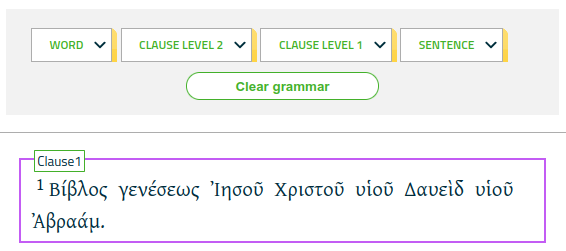
\includegraphics[width=0.5\textwidth]{clause1.png}
      \caption{The term ``Clause level 1'' is used in the grammar selection box, but ``Clause1'' is
        used in the text area.}\label{fig-clause1}
    }
  \end{center}
\end{figure}

As mentioned in Section \ref{sec-grammarfeature}, the ETCBC4 has a special feature name,
``\texttt{clause\_atom:code\_TYPE\_text}''. This requests a textual interpretation of the
\emph{code} feature which in reality is an integer value. The translation from integer to string is
handled by a special structure in the localization information for the Emdros object
\emph{clause\_atom,} as shown in Listing \ref{list-clause-atom-code}.


\begin{lstlisting}[numbers=left,caption=Handling integer to text translation,label=list-clause-atom-code]
        "clause_atom": {
            "_objname": "Clause atom",
            "code_TYPE_text": "Linkage",
            "code_TYPE_text_VALUES": [
                {
                    "first": 0,
                    "last": 0,
                    "text": "No relation"
                },
                {
                    "first": 10,
                    "last": 16,
                    "text": "Relative"
                },
                {
                    "first": 50,
                    "last": 74,
                    "text": "Inf.constr."
                },
                ... %\textrm{\scriptsize(Additional ranges omitted)}%
            ]
            ... %\textrm{\scriptsize(Additional features omitted)}%
        }
\end{lstlisting}

Here, the name ``\texttt{code\_TYPE\_text\_VALUES}'' identifies ranges of integer values that should
be presented textually as a particular text. For example, if the value of the \emph{code} feature is
between 10 and 16 (inclusive), the corresponding text is \emph{``Relative''.}

\subsection{The \emph{emdrostype} Key}\label{enum-loc}\index{emdrostype|hyperit}

The value of \emph{emdrostype} is a collection of key/value pairs containing the localized names for
the value of Emdros enumeration\index{Emdros!enumeration} types. As an example, Listing \ref{list-emdrostype-sample} shows
a subset of the \emph{emdrostype} for English localization of the ETCBC4 database.

\begin{lstlisting}[numbers=left,caption=A sample emdrostype value,label=list-emdrostype-sample]
    "emdrostype": {
        "part_of_speech_t": {%\label{line-pos-start}%
            "verb": "Verb",
            "subs": "Noun",
            "nmpr": "Proper noun",
            ... %\textrm{\scriptsize(Additional values omitted)}%
        },%\label{line-pos-end}%
        "gender_t": {%\label{line-gender-start}%
            "f": "#2 Feminine",
            "m": "#1 Masculine",
            "NA": "#3 None",
            "unknown": "#4 Unknown"
        },%\label{line-gender-end}%
        ... %\textrm{\scriptsize(Additional enumeration types omitted)}%
    }
\end{lstlisting}

Each key within the \emph{emdrostype} is the name of an Emdros enumeration type, so the above
example gives information about the \emph{part\_of\_speech\_t} and the \emph{gender\_t} enumeration
types.

Each key has a value which is a collection of key/value pairs, giving the names and the English
translation of the values of the enumeration type.

In the above example, lines \ref{line-pos-start}-\ref{line-pos-end} indicate that the type
\emph{part\_of\_speech\_t} has values such as \emph{verb, subs,} and \emph{nmpr}, whose English
translations are ``Verb'', ``Noun'', and ``Proper~noun'', respectively.

Lines \ref{line-gender-start}-\ref{line-gender-end} indicate that type \emph{gender\_t} has values
\emph{f, m, NA,} and \emph{unknown}, whose English translations are ``Feminine'', ``Masculine'',
``None'', and ``Unknown'', respectively. The strings ``\#1'', ``\#2'' etc. indicate the order in
which these values should be sorted when presented to the user. Normally, the values would be sorted
alphabetically thus:

\begin{center}
  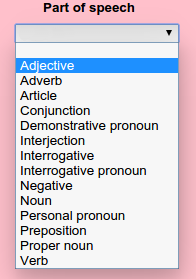
\includegraphics[width=0.3\textwidth]{psp.png}
\end{center}

But if the English translation starts with ``\#1'', ``\#2'' etc. these numbers indicate the sort
order. So with the contents of \emph{gender\_t} given in Listing \ref{list-emdrostype-sample},
genders are sorted thus:

\begin{center}
  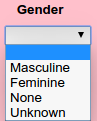
\includegraphics[width=0.148\textwidth]{gender.png}
\end{center}


If the translation of an enumeration value is long, it may not display well in the text area.
Abbreviated versions may be provided by appending the string \emph{\_abbrev} to the key in the
\emph{emdrostype}. This can be seen in Listing \ref{list-emdrostype-abbrev}, which is taken from
the English localization of the \emph{nestle1904} database.

\begin{lstlisting}[numbers=left,caption=Abbreviated emdrostype values,label=list-emdrostype-abbrev]
    "emdrostype": {
        "clause_type_t": {
            "ADV": "Adverbial",
            "CL": "Clause",
            ... %\textrm{\scriptsize(Additional enumeration values omitted)}%
        },
        "clause_type_t_abbrev": {
            "ADV": "ADV",
            "CL": "CL",
            ... %\textrm{\scriptsize(Additional enumeration values omitted)}%
        },
        ... %\textrm{\scriptsize(Additional enumeration types omitted)}%
    }
\end{lstlisting}

In this listing the enumeration value \emph{ADV} of type \emph{clause\_type\_t} is normally translated ``Adverbial'', but in
the text display area it is simply ``ADV'', as shown in Figure \ref{fig-clause2}.

\begin{center}
  \parbox{0.7\textwidth}{
    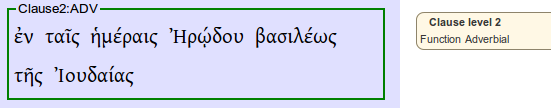
\includegraphics[width=0.7\textwidth]{clause2.png}
    \captionof{figure}{The term ``Adverbial'' is used in the grammar information box, but ``ADV'' is
      used in the text area.}\label{fig-clause2}
  }
\end{center}


\subsection{The \emph{grammarfeature, grammarmetafeature, grammarsubfeature,} and \emph{grammargroup} Keys}%
\label{grammar-loc}\index{GrammarFeature}\index{GrammarMetaFeature}\index{GrammarSubFeature}\index{GrammarGroup}

Section \ref{sentencegrammar} describes how the Database Specification File specifies how grammar
information should be grouped in the grammar selection box and the grammar information box on the
Bible OL webpage. Sections \ref{sec-grammarfeature}, \ref{sec-grammarmetafeature}, and
\ref{sec-grammargroup} describe the GrammarFeature, GrammarMetaFeature, and GrammarGroup
specifications and the GrammarSubFeature which is part of a GrammarMetaFeature.

In the Grammar Localization Structure, the \emph{grammarfeature, grammarmetafeature, grammargroup,} and
\emph{grammarsubfeature} keys give the translation of these items, as detailed below.

\subsubsection{\emph{grammarfeature}}

As an example, Listing \ref{list-grammarfeature-sample} shows the \emph{grammarfeature} for the
English localization of the ETCBC4 database.

\begin{lstlisting}[caption=A sample grammarfeature value,label=list-grammarfeature-sample]
    "grammarfeature": {
        "word": {
            "text_translit": "Transliteration"
        }
    }
\end{lstlisting}

Section \ref{emdrosobject-loc} describes how the \emph{emdrosobject}\index{emdrosobject} key is used
to provide translations for Emdros object features. The \emph{grammarfeature} in the above example
gives an alternative translation. Normally the translation of a feature is taken from
\emph{emdrosobject}, but in the case of the grammar selection box\index{grammar selection box} and
the grammar information box\index{grammar information box}, the translation in \emph{grammarfeature}
is used, if present. If no translation is given in \emph{grammarfeature}, the translation from
\emph{emdrosobject} is used.


\subsubsection{\emph{grammarmetafeature}}\index{GrammarMetaFeature}

Listing \ref{list-grammarmetafeature-sample} shows the \emph{grammarmetafeature} for the English
localization of the ETCBC4 database.

\begin{lstlisting}[numbers=left,caption=A sample grammarmetafeature value,label=list-grammarmetafeature-sample]
    "grammarmetafeature": {
        "word": {
            "pgn": "Person, gender, number",%\label{line-pgn}%
            "suffix_pgn": "Suffix: Person, gender, number"
        }
    }
\end{lstlisting}

In line \ref{line-pgn} the GrammarMetaFeature \emph{pgn} of the \emph{word} object is given the
English translation ``Person, gender, number''. (Listing \ref{list-gmf-sample} on page
\pageref{list-gmf-sample} specifies that the \emph{word} object has a GrammarMetaFeature called
\emph{pgn}.)

\subsubsection{\emph{grammarsubfeature}}\index{GrammarSubFeature}

Listing \ref{list-grammarsubfeature-sample} shows a subset of the \emph{grammarsubfeature} for the
English localization of the ETCBC4 database.

\begin{lstlisting}[caption=A sample grammarsubfeature value,label=list-grammarsubfeature-sample]
    "grammarsubfeature": {
        "word": {
            "ps": {
                "p1": "1",
                "NA": "-",
                "p2": "2",
                "p3": "3",
                "unknown": "?"
            },
            "gn": {
                "f": "F",
                "m": "M",
                "NA": "-",
                "unknown": "?"
            },
            "nu": {
                "du": "Du",
                "NA": "-",
                "pl": "Pl",
                "sg": "Sg",
                "unknown": "?"
            },
            ... %\textrm{\scriptsize(Additional features omitted)}%
        }
    }
\end{lstlisting}

The example in Listing \ref{list-gmf-sample} on page \pageref{list-gmf-sample} specifies that the
\emph{word} object has a GrammarMetaFeature called \emph{pgn} which is made up of the
GrammarSubFeatures \emph{ps, gn,} and \emph{nu}. The \emph{grammarsubfeature} value in Listing
\ref{list-grammarsubfeature-sample} above specifies the English translation for these three
GrammarSubFeatures. So if, for example, a word has features \emph{ps=p2, gn=m,} and \emph{nu=sg}
(corresponding to second person, masculine, singular), the \emph{pgn} GrammarMetaFeature should be
rendered as ``2MSg''.


\subsubsection{\emph{grammargroup}}\index{GrammarGroup}

Listing \ref{list-grammargroup-sample} shows the \emph{grammargroup} for the English localization of
the ETCBC4 database.

\begin{lstlisting}[caption=A sample grammargroup value,label=list-grammargroup-sample]
    "grammargroup": {
        "word": {
            "form_in_text": "Form in text",
            "lexeme": "Lexeme",
            "morphology": "Morphology"
        }
    },
\end{lstlisting}

The Database Specification File for the ETCBC4 database defines three GrammarGroups for the
\emph{word} object with the names \emph{form\_in\_text,\footnote{Shown in Listing
    \ref{list-itemssample} on page \pageref{list-itemssample}.} lexeme,} and \emph{morphology.} The
localization information above specifies the English names for these GrammarGroups. The two
illustrations in Section \ref{sentencegrammar} show these translations in the grammar selection
box\index{grammar selection box} and the grammar information box\index{grammar information box}.

\subsection{The \emph{universe} Key}\label{universe-loc}\index{passages}

The value of \emph{universe} is collection of key/value pairs describing how to display book,
chapter, and verse references.

As an example, Listing \ref{list-universe-sample} shows a subset of the \emph{universe} for English
localization of the ETCBC4 database.

\begin{lstlisting}[escapechar=\#,numbers=left,caption=A subset of the universe value,label=list-universe-sample]
    "universe": {
        "book": {
            "_label": "%s", #\label{line-book-label}#
            "Genesis": "Genesis", #\label{line-first-book}#
            "Exodus": "Exodus",
            "Leviticus": "Leviticus",
            "Numeri": "Numbers",
            "Deuteronomium": "Deuteronomy",
            "Josua": "Joshua",
            "Judices": "Judges",
            "Ruth": "Ruth",
            "Samuel_I": "1 Samuel",
            "Samuel_II": "2 Samuel",
            ... #\textrm{\scriptsize(Additional books omitted)}\label{line-last-book}#
        },
        "chapter": {
            "_label": "Chapter %s" #\label{line-chapter-label}#
        },
        "verse": {
            "_label": "Verse %s" #\label{line-verse-label}#
        },
        "reference": {
            "_label": "%s %d:%d", #\label{line-reference-label}#
            "Genesis": "Gen", #\label{line-first-book-abbrev}#
            "Exodus": "Ex",
            ... #\textrm{\scriptsize(Additional book abbreviations omitted)}\label{line-last-book-abbrev}#
        }
    }
\end{lstlisting}

The \emph{universeHierarchy} key of the Database Specification File (see page
\pageref{universe-hierarchy}) defines the reference hierarchy of ETCBC4 as consisting of the Emdros
object types \emph{book, chapter,} and \emph{verse.} The \emph{universe} key in Listing
\ref{list-universe-sample} above defines how these three object types should be rendered:

The \emph{\_label} key presents the general format as a string where ``\%s'' is to be replaced by
the actual reference. So, when line \ref{line-chapter-label} gives the \emph{\_label} key of
\emph{chapter} a value of ``Chapter~\%s'', it means that chapter 18 will be displayed as
``Chapter~18''.

For the \emph{book} object, the \emph{\_label} key (line \ref{line-book-label}) is simply the string
``\%s'', but additionally English translations of the book names used in ETCBC4 are given in lines
\ref{line-first-book}-\ref{line-last-book}.

The \emph{reference} key specifies how a Bible reference should be written. The \emph{\_label} key
here (line \ref{line-reference-label}) specifies the format as ``\%s \%d:\%d''. The ``\%s'' will be
replaced by the abbreviated book name, and the two ``\%d'' strings will be replaced by the chapter
and verse number, respecitively. Lines \ref{line-first-book-abbrev}-\ref{line-last-book-abbrev}
contain abbreviations of the book names.


%%%%%%%%%%%%%%%%%%%% Grammar Localization Comments %%%%%%%%%%%%%%%%%%%%
\section{Grammar Localization Comments}\label{sec-gram-loc-comments}\index{grammar localization comments|hyperit}

In addition to the Grammar Localization Structures for various target languages, the
\emph{db\_localize} table also contains comments for the different structures. These comments are
found in entries where the \emph{lang} field is ``comment''.

The grammar localization comments are structured exactly as the Grammar Localization Structures, but
their contents are used in the translator's interface to guide in the translation of each item.
Additionally, if a value starts with the string ``f:textarea'', the translator's interface will use
a \xml{textarea} HTML element for input. Otherwise, the translator's interface will use an
\xml{input type="text"} HTML element.


%%%%%%%%%%%%%%%%%%%% Lexicon Localization %%%%%%%%%%%%%%%%%%%%
\section{Lexicon Localization}\label{sec-lex-loc}\index{lexicon localization|hyperit}

Sections \ref{sec-lexicon-heb}, \ref{sec-lexicon-heb-lang}, \ref{sec-lexicon-greek}, and
\ref{sec-lexicon-greek-lang} give information about how localized versions of the Hebrew, Aramaic,
and Greek dictionaries are stored.


%%%%%%%%%%%%%%%%%%%% Importing and Exporting Translations %%%%%%%%%%%%%%%%%%%%
\section{Importing and Exporting Translations}\label{sec-imp-exp-trans}%
\index{importing translations|hyperit}\index{exporting translations|hyperit}%
\index{translations!importing and exporting|hyperit}

For a translator, it is often more convenient to work with translations offline. For this reason it
is possble to import and export the various translation tables from and to a textual format.

\subsection{The User Interface}

Sections \ref{sec-language-comment} and \ref{sec-language-lang} describe how localization of the
user interface is stored in the user database.

From the shell command line on the server the contents of the user interface tables can be exported
thus:

\begin{lstlisting}[language=bash,basicstyle={\ttfamily}]
php index.php translate if_db2php %\textrm{\textit{language-code}}% %\textrm{\textit{destination-directory}}%
\end{lstlisting}

\noindent
or thus:

\begin{lstlisting}[language=bash,basicstyle={\ttfamily}]
php index.php translate if_db2php %\textrm{\textit{language-code}\_\textit{variant}}% %\textrm{\textit{destination-directory}}%
\end{lstlisting}


Here \emph{language-code} is, for example, ``en'' for English or ``comment'' to get the comment
information (see Section \ref{sec-language-comment}). The optional \emph{variant} gives you a
language variant (note that an underscore rather than a space separates the language code from the
variant). The exported files will be stored in a directory named
\emph{destination-directory/language-code}. (The directory \emph{destination-directory} must exist,
the directory \emph{destination-directory/language-code} need not exist.)

To import the user interface tables from textual files, execute this command from the shell command
line on the server:

\begin{lstlisting}[language=bash,basicstyle={\ttfamily}]
php index.php translate if_php2db [-i] %\textrm{\textit{language-code}}% %\textrm{\textit{source-directory}}%
\end{lstlisting}


\noindent
or this command:

\begin{lstlisting}[language=bash,basicstyle={\ttfamily}]
php index.php translate if_php2db [-i] %\textrm{\textit{language-code}\_\textit{variant}}% %\textrm{\textit{source-directory}}%
\end{lstlisting}

The imported files will be loaded from a directory named \emph{source-directory}.

If the optional parameter \texttt{-i} is absent, all translation strings in the database are
replaced by the translations found in the source directory. If the parameter \texttt{-i} is present,
only translations that are not already in the database are added; in this case the command will warn
about translations that differ in the database and the source directory.

Note the difference in directory naming in the export and import commands. The language code is
appended to the directory name on export, but not on import. To export the English
texts to a directory called \texttt{abc} and import it again, use this sequence of commands:

\begin{lstlisting}[language=bash,basicstyle={\ttfamily}]
php index.php translate if_db2php en abc
php index.php translate if_php2db en abc/en
\end{lstlisting}

The reason for this difference is that we want to enforce a particular directory structure when
exporting, but we cannot rely on having that structure when importing.

\subsection{Grammar Localization Structures}

Section \ref{sec-gram-loc-struct} describes how localization of grammar information is stored in the
user database.

From the shell command line on the server the contents of all the grammar localization structures can be exported
thus:

\begin{lstlisting}[language=bash,basicstyle={\ttfamily}]
php index.php translate gram_db2prop %\textrm{\textit{destination-directory}}%
\end{lstlisting}

\noindent
or thus:

\begin{lstlisting}[language=bash,basicstyle={\ttfamily}]
php index.php translate gram_db2prop %\textrm{\textit{destination-directory}}% %\textrm{\textit{variant}}%
\end{lstlisting}

This command will store the grammar localization structures for all Emdros databases and all
languages in files in the directory \emph{destination-directory} (which must exist). The data will
be stored in ``pretty'' JSON format. If \emph{variant} is specified, data from that variant
translation will be used.

To import the grammar localization structures from textual files, place the JSON files in the directory
\texttt{db/propterty\_files} under the Bible OL main directory. Then execute this command from the
shell command line on the server:

\begin{lstlisting}[language=bash,basicstyle={\ttfamily}]
php index.php translate gram_prop2db %\textrm{\textit{source-directory}}%
\end{lstlisting}

\noindent
or this command:

\begin{lstlisting}[language=bash,basicstyle={\ttfamily}]
php index.php translate gram_prop2db %\textrm{\textit{source-directory}}% %\textrm{\textit{variant}}%
\end{lstlisting}

This command will read the files from the \emph{source-directory} and update the contents of the
user database, where necessary. The command will print a list of tile files found plus information
about whether the contents of the files caused the database to be updated. If \emph{variant} is
specified, then that variant will be updated.

(In earlier versions of Bible OL, the \texttt{gram\_prop2db} command did not take a
\emph{source-directory} parameter; instead the \texttt{db/propterty\_files} directory was always used.)

\subsection{Lexicon}

Sections \ref{sec-lexicon-heb}, \ref{sec-lexicon-heb-lang}, \ref{sec-lexicon-greek}, and
\ref{sec-lexicon-greek-lang} describe how localized versions of the dictionaries are stored.

From the shell command line on the server the contents of a lexicon can be exported thus:

\begin{lstlisting}[language=bash,basicstyle={\ttfamily}]
php index.php translate download_lex %\textrm{\textit{source-language}}% %\textrm{\textit{target-language}}%
\end{lstlisting}

\noindent
or thus:

\begin{lstlisting}[language=bash,basicstyle={\ttfamily}]
php index.php translate download_lex %\textrm{\textit{source-language}}% %\textrm{\textit{target-language}}% %\textrm{\textit{variant}}%
\end{lstlisting}

The \emph{source-language} must be either ``heb'', ``aram'', or ``greek''. The
\emph{destination-language} must be, for example, ``en'' for English. The lexicon will be written to
the standard output as a comma-separated file, suitable for import into a spreadsheet program. If \emph{variant} is
specified, data from that variant translation will be used.

Note that a user with translator or administrator privileges can also download the lexicons from the
Bible OL website by selecting the \emph{Administration > Download lexicon} menu.

A lexicon can be imported from the shell command line on the server by executing this command:

\begin{lstlisting}[language=bash,basicstyle={\ttfamily}]
php index.php translate import_lex %\textrm{\textit{source-language}}% %\textrm{\textit{target-language}}% %\textrm{\textit{CSV-file}}%
\end{lstlisting}

\noindent
or this command:

\begin{lstlisting}[language=bash,basicstyle={\ttfamily}]
php index.php translate import_lex %\textrm{\textit{source-language}}% %\textrm{\textit{target-language}}% %\textrm{\textit{CSV-file}}% %\textrm{\textit{variant}}%
\end{lstlisting}


The \emph{source-language} and \emph{destination-language} are described above. The \emph{CSV-file}
is the name of a comma-separated file containing the lexicon in the exact format generated by the export line
above. This means that the imported CSV file must have the same number of fields and the same
headings as the generated file.  If \emph{variant} is
specified, then that variant will be updated.




%%%%%%%%%%%%%%%%%%%%%%%%%%%%%%%%%%%%%%%%%%%%%%%%%%
%%%%%%%%%%%%%%%%%%%% Plug-ins %%%%%%%%%%%%%%%%%%%%
\chapter{Plug-ins}\index{plug-in}

\textbf{Read this chapter if you want to modify Learning Journey or write a new plug-in.}
\plainbreak{3}

CodeIgniter and Bible OL provide a limited mechanism for writing plug-ins (that is, extensions to
the system).

PHP code for the plug-in must be stored in a directory hierarchy under
\texttt{myapp/third\_party/xxx}, where \texttt{xxx} is the name of the plug-in. The directory
hierachy must contain the directories required by CodeIgniter, namely, \texttt{controllers},
\texttt{helpers}, \texttt{language}, \texttt{libraries}, \texttt{models}, and \texttt{views}.

The names of the controllers in the \texttt{controllers} directory must start with the string
``Ctrl\_XXX\_'', where ``XXX'' is the name of the plug-in in upper case letters. Similarly the
models and views should have names that start with the string ``Mod\_XXX\_'' or ``view\_XXX\_''.

Localization of plug-ins is not quite streamlined yet. Localization information can be stored in the
\texttt{language} directory.

To enable a plugin with the name ``xxx'', the following modifications must be made to the Bible OL
code:

In the file \texttt{myapp/config/config.php} add the following line:

\begin{lstlisting}[language=PHP]
$config['xxx_enabled'] = true;
\end{lstlisting}

The value can be set to \emph{true} or \emph{false} depending on whether the plug-in is installed or
not.

In the file \texttt{myapp/config/autoload.php} add the following lines:

\begin{lstlisting}[language=PHP]
if (config_item('xxx_enabled'))
    $autoload['packages'][] = APPPATH.'third_party/xxx';
\end{lstlisting}

In the file \texttt{myapp/config/routes.php} add the following lines:

\begin{lstlisting}[language=PHP]
if ($this->config->item('xxx_enabled')) {
    $route['(xxx)/(.+)'] = function ($name, $path) {
        $this->directory="../third_party/$name/controllers/"; // $this is the CI_Router object
        return "Ctrl_$path";
    };
}
\end{lstlisting}

This ensures that URLs such as, for example, \texttt{'https://bibleol.3bmoodle.dk/xxx/XXX\_foobar} is
sent to the controller at \texttt{myapp/third\_party/xxx/controllers/Ctrl\_XXX\_foobar}. Thus, all
URLs directed at plug-in ``xxx'' should start with the string ``/xxx/'' after the hostname.

If additional code needs to be added to Bible OL (for example, to add special menu items if a plug-in
is available), the following can be added to the existing Bible OL code:

\begin{lstlisting}[escapechar=\#,language=PHP]
if ($this->config->item('xxx_enabled')) {
   ...#\textrm{\scriptsize(Code that uses the plug-in)}#
}
\end{lstlisting}


At present, the only available plug-in is \emph{Learning Journey}. 

%%%%%%%%%%%%%%%%%%%% The Learning Journey Plug-in %%%%%%%%%%%%%%%%%%%%
\section{The Learning Journey Plug-in}\label{sec-lj}\index{Learning Journey}

Bible OL collects information about the answers users give to exercises and how much time they spend
on each exercise. The Learning Journey plug-in%
\footnote{Developed by Judith Gottschalk.\index{Gottschalk, Judith}}
accesses this information and provides statistics\index{statistics} about each user's
performance.

No further information about Learning Journey is given in this document.




%%%%%%%%%%%%%%%%%%%%%%%%%%%%%%%%%%%%%%%%%%%%%%%%%%%%%%%%%%%%%%%%
%%%%%%%%%%%%%%%%%%%% Complementary Websites %%%%%%%%%%%%%%%%%%%%
\chapter{Complementary Websites}

\textbf{Read this chapter if you want to.}
\plainbreak{3}


A few additional websites complement the function of Bible OL: The resource website and the SHEBANQ
website.



%%%%%%%%%%%%%%%%%%%% The Resource Website %%%%%%%%%%%%%%%%%%%%
\section{The Resource Website}\label{sec-resource-web}\index{resource website|hyperit}

The resource web site is a collection of photos from the Middle East. Many of them relate to events
and places described in the Bible. The photos have descriptive texts that contain Bible references.
The URL of the resource website is \url{http://resources.3bmoodle.dk}.

Bible OL can use information from the resource website to add picture links to Bible passages. If a
photo in the resource website refers to, for example, \bibleref{Exodus}{3}{2}, and a user ticks the
``Show link icons'' checkbox when displaying Exodus chapter 3, a green ``P'' icon will appear in the
text next to verse 2:

\begin{center}
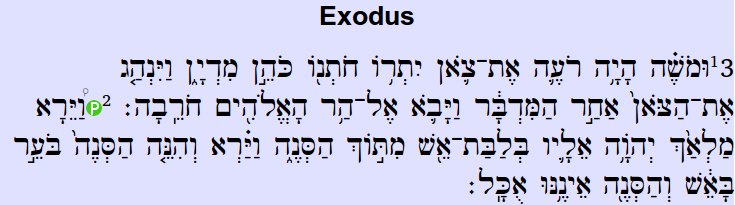
\includegraphics[width=0.9\textwidth]{exodus3.png}
\end{center}

Clicking on the icon will cause the web browser to display the relevant photo. If there are more
than one photo, the icon will be blue rather than green.

Bible OL gathers information about the photos on the resource web site by executing the command

\begin{lstlisting}[language=bash,frame=,basicstyle={\ttfamily}]
php index.php pic2db
\end{lstlisting}

\noindent
in a cron\index{cron job} job. This command calls Bible OL's \emph{Ctrl\_pic2db} controller (in the file
\texttt{myapp/\allowbreak{}controllers/\allowbreak{}ctrl\_pic2db.php}), which requests information from the resource database.

By accessing the URL \url{http://resources.3bmoodle.dk/jsonrefs.php}, the \emph{Ctrl\_pic2db}
controller receives a JSON object from the resources website containing information about the photos
and the Bible verses to which they refer. Bible OL stores this information in the
\emph{bible\_refs}\index{bible\_refs table} table in the user database\index{user database} (see Section
\ref{sec-bible-refs}).

In addition to the pictures, the resource website may also provide URLs associated with various
Bible verses. These URLs are configured in the resource website but are otherwise unrelated to the
functioning of that website. The URLs are intended to identify videos, documents, or other resources
that may relevant for studying a particular verse.

Information about these URLs is also retrieved by the cron job above. By accessing the URL
\url{http://resources.3bmoodle.dk/jsonurls.php}, the \emph{Ctrl\_pic2db} controller receives a JSON
object from the resources website containing information about the URLs and the Bible verses to
which they refer. Bible OL stores this information in the \emph{bible\_urls}%
\index{bible\_urls table}
table in the user database\index{user database} (see Section \ref{sec-bible-urls}). Links to these
urls are displayed as ``V'', ``D'', or ``U'' icons.

%%%%%%%%%%%%%%%%%%%% The SHEBANQ Website %%%%%%%%%%%%%%%%%%%%
\section{The SHEBANQ Website}\label{sec-shebanq}\index{SHEBANQ}

SHEBANQ (System for HEBrew text: ANnotations for Queries and markup) is a website that uses the
ETCBC4 database for displaying text and grammar information for the Hebrew Bible. The URL is
\url{http://shebanq.ancient-data.org}.

When Bible OL displays a text from the Old Testament, an icon in the upper right corner of the text
area provides a link to the same chapter at the SHEBANQ website. A similar link to Bible OL is found
on the SHEBANQ website. Also, when a teacher is creating an exercise in Bible OL, they can import
MQL queries from the SHEBANQ website (see Section \ref{sec-shebanq-import}).


%%%%%%%%%%%%%%%%%%%%%%%%%%%%%%%%%%%%%%%%%%%%%%%%%%%%%%%%%%%%%%%%%%
%%%%%%%%%%%%%%%%%%%% Appendix: ETCBC4 Details %%%%%%%%%%%%%%%%%%%%
\appendix
\chapter{ETCBC4 Details}\label{app-etcbc}\index{ETCBC4|hyperit}

The \emph{ETCBC4} Emdros database contains the Hebrew and Aramaic text for the Old
Testament.\index{Old Testament}

The database comes from the \emph{Eep Talstra Center for Bible and Computer}%
\index{Eep Talstra Center for Bible and Computer}
and is made available under a Creative Commons Attribution-NonCommercial 4.0 International
License\index{license}.\footnote{\url{http://creativecommons.org/licenses/by-nc/4.0}.} When
describing the database, a text similar to this one should be used: ``The database itself can be
found through this persistent identifier: \texttt{urn:nbn:nl:ui:13-048i-71}.'' The identifier should
be a hyperlink pointing to
\url{http://www.persistent-identifier.nl/?identifier=urn:nbn:nl:ui:13-048i-71}.

Prior to using this database in Bible OL, I have added additional features to the information from
its original creators. More details about this is given in Section \ref{etcbc-origin}.

%%%%%%%%%%%%%%%%%%%% The word Object %%%%%%%%%%%%%%%%%%%%
\section{The \emph{word} Object}\index{word}

The basic object\index{Emdros!object} type is the \emph{word}. Each \emph{word} corresponds to a
single monad\index{monad}. The following sections give details about the
features\index{Emdros!feature} of the object.

Many of the features exist in several different encodings. The encodings are indicated by the name
of the feature. A feature \emph{XXX} may exists in these variants:

\begin{my-tabu}{ll}{ \headii{Feature name}{Encoding} }
  XXX & Transcribed alphabet\index{alphabet!transcribed}\\
  XXX\_utf8 & Native alphabet\index{alphabet!native}\\
  XXX\_translit & Transliterated alphabet\index{alphabet!transliterated}\\
  XXX\_cons\_utf8 & Consonants only, native alphabet\\
  XXX\_nocant & Cantillation marks omitted, transcribed alphabet\\
  XXX\_nocant\_utf8 & Cantillation marks omitted, native alphabet\\
  XXX\_nopunct\_translit & Punctuation omitted, transliterated alphabet\\
\end{my-tabu}

Except where otherwise noted, all features of the \emph{word} object are string features.

In cases where a feature is an enumeration\index{Emdros!enumeration}, the enumeration type may
contain values that are not actually used. Such values are not listed in the following sections.

\subsection{Features: g\_word, g\_suffix, and g\_cons}\label{suffix}

These features relate to the visual appearance of a word.

The \emph{g\_word} features contain the actual text of the word. These variants exist:

\begin{itemize}
\item g\_word
\item g\_word\_utf8
\item g\_word\_translit
\item g\_word\_cons\_utf8
\item g\_word\_nocant
\item g\_word\_nocant\_utf8
\item g\_word\_nopunct\_translit
\end{itemize}

The \emph{g\_word} features work together with the \emph{g\_suffix}\index{suffix} features as
described in Section \ref{sec-contin}. The \emph{g\_suffix} features exist in these variants:

\begin{itemize}
\item g\_suffix
\item g\_suffix\_utf8
\item g\_suffix\_translit
\end{itemize}

The \emph{g\_suffix} features contain characters that follow a word. Possible suffixes are:

\begin{itemize}
\item An empty string
\item A space
\item \heb{־}
\item \heb{׀}\quad followed by a space
\item \heb{׃}\quad followed by a space
\item \heb{׃ ׆}\quad followed by a space
\item \heb{׃ ׆ ס}\quad followed by a space
\item \heb{׃ ׆ פ}\quad followed by a space
\item \heb{׃ ס}\quad followed by a space
\item \heb{׃ פ}\quad followed by a space
\item \heb{ס}\quad surrounded by spaces
\item \heb{פ}\quad surrounded by spaces 
\end{itemize}

Note: Do not confuse the \emph{g\_suffix} features with the features \emph{suffix\_gender,} \emph{suffix\_number,} and
\emph{suffix\_person} which are described in Section \ref{suffix-gram}.


The \emph{g\_cons} features contain the consonants of the word. They are not used by Bible OL
because their information is available by other means.

The \emph{g\_cons} features exist in these variants:

\begin{itemize}
\item g\_cons
\item g\_cons\_utf8
\end{itemize}


\subsection{Features: g\_lex, lex, and g\_voc\_lex}

The ``lexeme''\index{lexeme|hyperit} or ``lemma''\index{lemma|see {lexeme}} of a word is the version of
the word found in a dictionary. For example, the English word ``mice'' has the lexeme ``mouse''
because in a dictionary, the word is found under the entry ``mouse''.

ETCBC4 has three different lexeme features with different characteristics.

The \emph{g\_voc\_lex} is the word commonly taken to be the lexeme of a Hebrew word. Except
for verbs, this lexeme contains vowels. The \emph{g\_voc\_lex} features exist in these variants:

\begin{itemize}
\item g\_voc\_lex
\item g\_voc\_lex\_utf8
\item g\_voc\_lex\_translit
\item g\_voc\_lex\_cons\_utf8
\end{itemize}

The \emph{g\_lex} and \emph{lex} features contain various other ways to write the lexeme. Compare,
for example, these three lexemes for \heb{אֱלֹהִים}:

\begin{center}
  \begin{tabular}{ll}
    \textbf{Feature name} & \textbf{Content}\\
    \hline
    g\_voc\_lex\_utf8 & \heb{אֱלֹהִים}\\
    g\_lex\_utf8 & \heb{אֱלֹה}\\
    lex\_utf8 & \heb{אלהים֜}
  \end{tabular}
\end{center}

I have not studied all the differences between the three lexemes. Suffice it to say that
\emph{g\_voc\_lex\_utf8} is the one normally shown to users, and \emph{lex} is useful
internally in the system because it only contains consonants and uses the transcribed alphabet.

The \emph{g\_lex} features exist in these variants:

\begin{itemize}
\item g\_lex
\item g\_lex\_utf8
\item g\_lex\_cons\_utf8
\end{itemize}

The \emph{lex} features exist in these variants:

\begin{itemize}
\item lex
\item lex\_utf8
\item lex\_cons\_utf8
\end{itemize}

\subsection{Features: lexeme\_occurrences and frequency\_rank}

ETCBC4 contains information about the frequency of various lexemes\index{lexeme}. The feature
\emph{lexeme\_occurrences} is an integer feature containing the number of times this lexeme
occurs in the Old Testament. The feature \emph{frequency\_rank} is an integer feature containing the
rank of each lexeme: The most frequent lexeme has rank 1, the second most frequent lexeme has rank
2, etc.

These two features are counted separately for Hebrew and Aramaic parts of the Old Testament. 


\subsection{Features: pfm, g\_pfm}

The \emph{pfm} feature describes the paradigmatic form of the preformative. The following values are
possible:

\begin{itemize}
\item The empty string
\item >
\item absent\footnote{This is the actual string ``absent''.}
\item H
\item J
\item L
\item M
\item N
\item n/a
\item T=
\item T
\end{itemize}

The \emph{g\_pfm} features contain the graphical representation of the preformative. These
features exist in these variants:

\begin{itemize}
\item g\_pfm
\item g\_pfm\_utf8
\item g\_pfm\_translit
\item g\_pfm\_cons\_utf8
\end{itemize}


\subsection{Features: vbs, g\_vbs}

The \emph{vbs} feature describes the paradigmatic form of the root formation morpheme. The following
values are possible:

\begin{itemize}
\item >
\item absent\footnote{This is the actual string ``absent''.}
\item C
\item H
\item HCT
\item HT
\item N
\item n/a
\item NT
\item >T
\item T
\end{itemize}

The \emph{g\_vbs} features contain the graphical representation of the root formation morpheme.
These features exist in these variants:

\begin{itemize}
\item g\_vbs
\item g\_vbs\_utf8
\item g\_vbs\_translit
\item g\_vbs\_cons\_utf8
\end{itemize}


\subsection{Features: vbe, g\_vbe}

The \emph{vbe} feature describes the paradigmatic form of the verbal ending. The following
values are possible:

\begin{itemize}
\item The empty string
\item H=
\item H
\item J
\item JN
\item N>
\item N
\item n/a
\item NH
\item NW
\item T==
\item T=
\item T
\item TJ
\item TM
\item TN
\item TWN
\item W
\item WN
\end{itemize}

The \emph{g\_vbe} features contain the graphical representation of the verbal ending.
These features exist in these variants:

\begin{itemize}
\item g\_vbe
\item g\_vbe\_utf8
\item g\_vbe\_translit
\item g\_vbe\_cons\_utf8
\end{itemize}

\subsection{Features: nme, g\_nme}

The \emph{nme} feature describes the paradigmatic form of the nominal ending. The following
values are possible:

\begin{itemize}
\item The empty string
\item absent\footnote{This is the actual string ``absent''.}
\item H
\item J=
\item J
\item JM=
\item JM
\item JN=
\item JN
\item N
\item n/a
\item T=
\item T
\item TJ
\item TJM
\item TJN
\item W=
\item W
\item WT
\item WTJ
\end{itemize}

The \emph{g\_nme} features contain the graphical representation of the nominal ending.
These features exist in these variants:

\begin{itemize}
\item g\_nme
\item g\_nme\_utf8
\item g\_nme\_translit
\item g\_nme\_cons\_utf8
\end{itemize}

\subsection{Features: uvf, g\_uvf}

The \emph{uvf} feature describes the paradigmatic form of the univalent final. The following
values are possible:

\begin{itemize}
\item >
\item absent\footnote{This is the actual string ``absent''.}
\item H
\item J
\item N
\item W
\end{itemize}

The \emph{g\_uvf} features contain the graphical representation of the univalent final.
These features exist in these variants:

\begin{itemize}
\item g\_uvf
\item g\_uvf\_utf8
\item g\_uvf\_translit
\item g\_uvf\_cons\_utf8
\end{itemize}


\subsection{Features: prs, g\_prs}\label{prs}

The \emph{prs} feature describes the paradigmatic form of the pronominal suffix. The following
values are possible:

\begin{itemize}
\item H  
\item H= 
\item HJ 
\item HM 
\item HN 
\item HW 
\item HWN
\item J  
\item K  
\item K= 
\item KM 
\item KN 
\item KWN
\item M  
\item MW 
\item n/a
\item N  
\item N> 
\item NJ 
\item NW 
\item W  
\end{itemize}


The \emph{g\_prs} features contain the graphical representation of the pronominal suffix.
These features exist in these variants:

\begin{itemize}
\item g\_prs
\item g\_prs\_utf8
\item g\_prs\_translit
\item g\_prs\_cons\_utf8
\end{itemize}


\subsection{Feature: qere}

The \emph{qere} features contain the qere reading for the current word, if any.

The \emph{qere} features exist in these variants:

\begin{itemize}
\item qere
\item qere\_utf8
\item qere\_translit
\end{itemize}

\subsection{Feature: language}

The \emph{language} feature indicates if the word is Hebrew or Aramaic. It is an enumeration feature
of type \emph{language\_t} whose value is either \emph{Hebrew} or \emph{Aramaic.}

\subsection{Features: sp and pdp}

The \emph{sp} feature indicates the part of speech of the word; the \emph{pdp} feature indicates the
phrase dependent part of speech. Both are enumeration features of type \emph{part\_of\_speech\_t}.
They can have these values:

\begin{my-tabu}{ll}{ \headii{Value}{Meaning} }
    adjv & Adjective             \\
    advb & Adverb                \\
    art  & Article               \\
    conj & Conjunction           \\
    inrg & Interrogative         \\
    intj & Interjection          \\
    nega & Negative              \\
    nmpr & Proper noun           \\
    prde & Demonstrative pronoun \\
    prep & Preposition           \\
    prin & Interrogative pronoun \\
    prps & Personal pronoun      \\
    subs & Noun                  \\
    verb & Verb                  \\
\end{my-tabu}

\subsection{Features: ps, nu, gn, suffix\_person, suffix\_number, suffix\_gender, prs\_ps, prs\_nu, prs\_gn}\label{suffix-gram}

The \emph{ps, nu,} and \emph{gn} features indicate the person, number, and gender, respectively, of
the word. They are enumeration features of type \emph{person\_t, number\_t,} and \emph{gender\_t}
respectively.

The \emph{suffix\_person, suffix\_number,} and \emph{suffix\_gender} features indicate the person,
number, and gender of an optional suffix on the word. (Note: Do not confuse these features with the
suffix features described in Section \ref{suffix}.)

The \emph{prs\_ps, prs\_nu,} and \emph{prs\_gn} features are identical to the \emph{suffix\_person,
  suffix\_number,} and \emph{suffix\_gender} features, respectively.

The \emph{person\_t} enumeration has these values:

\begin{my-tabu}{cl}{ \headii{Value}{Meaning} }
    p1      & First person   \\
    p2      & Second person  \\
    p3      & Third person   \\
    unknown & Unknown person \\
    NA      & Not applicable \\
\end{my-tabu}

\Needspace*{5cm}%
The \emph{number\_t} enumeration has these values:

\begin{my-tabu}{cl}{ \headii{Value}{Meaning} }
    sg      & Singular       \\
    du      & Dual           \\
    pl      & Plural         \\
    unknown & Unknown number \\
    NA      & Not applicable \\
\end{my-tabu}


\Needspace*{5cm}%
The \emph{gender\_t} enumeration has these values:

\begin{my-tabu}{cl}{ \headii{Value}{Meaning} }
    f       & Feminine       \\
    m       & Masculine      \\
    unknown & Unknown number \\
    NA      & Not applicable \\
\end{my-tabu}


\subsection{Feature: ls}

The \emph{ls} feature indicates the lexical set of the word. It is an enumeration feature of type
\emph{lexical\_set\_t} whose value is one of the following:

\begin{my-tabu}{ll}{ \headii{Value}{Meaning} }
    afad & Anaphoric adverb       \\
    card & Cardinal               \\
    cjad & Conjunctive adverb     \\
    focp & Focus particle         \\
    gntl & Gentilic               \\
    mult & Noun of multitude      \\
    nmcp & Copulative noun        \\
    nmdi & Distributive noun      \\
    none & None                   \\
    ordn & Ordinal                \\
    padv & Potential adverb       \\
    ppre & Potential preposition  \\
    ques & Interrogative particle \\
    quot & Quotation verb         \\
    vbcp & Copulative verb        \\
\end{my-tabu}

\subsection{Feature: vs}

The \emph{vs} feature indicates the verbal stem of the word. It is an enumeration feature of type
\emph{verbal\_stem\_t} whose value is one of the following:

\begin{my-longtabu}{lll}{ \headiii{Value}{Meaning}{Used in language} }
    afel  & Afel         & Aramaic             \\
    etpa  & Etpaal       & Both                \\
    etpe  & Etpeel       & Aramaic             \\
    haf   & Hafel        & Aramaic             \\
    hif   & Hifil        & Hebrew              \\
    hit   & Hitpael      & Hebrew              \\
    hof   & Hofal        & Both                \\
    hotp  & Hotpaal      & Hebrew              \\
    hsht  & Hishtafal    & Both                \\
    htpa  & Hitpaal      & Aramaic             \\
    htpe  & Hitpeel      & Aramaic             \\
    htpo  & Hitpoal      & Hebrew              \\
    nif   & Nifal        & Hebrew              \\
    nit   & Nitpael      & Hebrew              \\
    pael  & Pael         & Aramaic             \\
    pasq  & Passive Qal  & Hebrew              \\
    peal  & Peal         & Aramaic             \\
    peil  & Peil         & Aramaic             \\
    piel  & Piel         & Hebrew              \\
    poal  & Poal         & Hebrew              \\
    poel  & Poel         & Hebrew              \\
    pual  & Pual         & Hebrew              \\
    qal   & Qal          & Hebrew              \\
    shaf  & Shafel       & Aramaic             \\
    tif   & Tifal        & Hebrew              \\
    NA    & \multicolumn{2}{l}{Not applicable} \\
\end{my-longtabu}

\subsection{Feature: vt}

The \emph{vt} feature indicates the verbal tense of the word. It is an enumeration feature of type
\emph{verbal\_tense\_t} whose value is one of the following:

\begin{my-tabu}{ll}{ \headii{Value}{Meaning} }
    coho & Cohortative          \\
    emim & Emphatic imperative  \\
    impf & Imperfect            \\
    impv & Imperative           \\
    infa & Infinitive absolute  \\
    infc & Infinitive construct \\
    juss & Jussive              \\
    perf & Perfect              \\
    ptca & Participle           \\
    ptcp & Passive participle   \\
    wayq & Wayyiqtol            \\
    NA   & Not applicable       \\
\end{my-tabu}

\subsection{Feature: st}

The \emph{st} feature indicates the state of the word. It is an enumeration feature of type
\emph{state\_t} whose value is one of the following:

\begin{my-tabu}{cl}{ \headii{Value}{Meaning} }
    a  & Absolute       \\
    c  & Construct      \\
    e  & Emphatic       \\
    NA & Not applicable \\
\end{my-tabu}


\subsection{Feature: verb\_class}

The \emph{verb\_class} feature indicates the verb classes to which a word belongs. It is list of
values of the enumeration type \emph{verb\_class\_t} whose values are:

\begin{itemize}
\item analog\_i\_nun
\item analog\_i\_waw
\item four\_consonants
\item geminate
\item hjh\_xjh
\item i\_aleph
\item i\_guttural
\item i\_nun
\item i\_waw
\item i\_yod
\item ii\_guttural
\item ii\_waw
\item ii\_yod
\item iii\_aleph
\item iii\_guttural
\item iii\_he
\item regular
\end{itemize}

Although the values \emph{analog\_i\_nun}, \emph{analog\_i\_waw}, and \emph{hjh\_xjh} are values of
the \emph{verb\_class\_t} type, they are not used by any verb in the database.

\subsection{Features: number, distributional\_parent, functional\_parent, lexeme\_count}

These features are currently not used by Bible OL and are not documented here.

\subsection{The Origin of the Features}\label{etcbc-origin}

The following features of the \emph{word} object were part of the ETCBC4 database as I received it
from its creators:

\begin{center}
  \begin{tabular}{llll}
    distributional\_parent & g\_suffix         & lex           & ps             \\
    functional\_parent     & g\_suffix\_utf8   & lexeme\_count & qere           \\
    g\_cons                & g\_uvf            & lex\_utf8     & qere\_utf8     \\
    g\_cons\_utf8          & g\_uvf\_utf8      & ls            & sp             \\
    g\_lex                 & g\_vbe            & nme           & st             \\
    g\_lex\_utf8           & g\_vbe\_utf8      & nu            & suffix\_gender \\
    gn                     & g\_vbs            & number        & suffix\_number \\
    g\_nme                 & g\_vbs\_utf8      & pdp           & suffix\_person \\
    g\_nme\_utf8           & g\_voc\_lex       & pfm           & uvf            \\
    g\_pfm                 & g\_voc\_lex\_utf8 & prs           & vbe            \\
    g\_pfm\_utf8           & g\_word           & prs\_gn       & vbs            \\
    g\_prs                 & g\_word\_utf8     & prs\_nu       & vs             \\
    g\_prs\_utf8           & language          & prs\_ps       & vt             \\
  \end{tabular}
\end{center}

The following word features were generated by the program
\emph{emdros\_updater}\index{emdros\_updater} which is available at
\url{https://github.com/EzerIT/ETCBC4BibleOL}.

\begin{center}
  \begin{tabular}{lll}
    frequency\_rank     & g\_uvf\_cons\_utf8      & g\_word\_nocant            \\
    g\_lex\_cons\_utf8  & g\_uvf\_translit        & g\_word\_nocant\_utf8      \\
    g\_nme\_cons\_utf8  & g\_vbe\_cons\_utf8      & g\_word\_nopunct\_translit \\
    g\_nme\_translit    & g\_vbe\_translit        & g\_word\_translit          \\
    g\_pfm\_cons\_utf8  & g\_vbs\_cons\_utf8      & lex\_cons\_utf8            \\
    g\_pfm\_translit    & g\_vbs\_translit        & lexeme\_occurrences        \\
    g\_prs\_cons\_utf8  & g\_voc\_lex\_cons\_utf8 & qere\_translit             \\
    g\_prs\_translit    & g\_voc\_lex\_translit   & verb\_class                \\
    g\_suffix\_translit & g\_word\_cons\_utf8     &                            \\
  \end{tabular}
\end{center}

The \emph{emdros\_updater} and associated programs also performs a number of modifications to the
database, including adding the verbal tenses \emph{jussive, cohortative,} and \emph{emphatic
  imperative}. See the file \url{https://github.com/EzerIT/ETCBC4BibleOL/blob/master/README.md} for
details.

%%%%%%%%%%%%%%%%%%%% The Other Object Types %%%%%%%%%%%%%%%%%%%%
\section{The Other Object Types}

For information about the other object types in the ETCBC4 database, please consult the MQL code
used for generating the database. The MQL code can be seen by running the
\emph{mqldump}\index{mqldump} program as described on page \pageref{list-mqldump}.

%%%%%%%%%%%%%%%%%%%%%%%%%%%%%%%%%%%%%%%%%%%%%%%%%%%%%%%%%%%%%%%%%%%%%%%%%
%%%%%%%%%%%%%%%%%%%% Appendix: ETCBC4 Words Database %%%%%%%%%%%%%%%%%%%%
\chapter{ETCBC4 Words Database}\label{app-worddb}\index{Words Database}

The Words Database (see Chapter \ref{chap-multiple-choice}) for the ETCBC4 Emdros database
has the name \texttt{ETCBC4\_words.db}. Its structure is defined by these SQL statements:

\begin{lstlisting}[language=SQL]
CREATE TABLE lexemes (id integer primary key, lex text);
CREATE TABLE lexsuf (id integer primary key, lexid integer, sufid integer);
CREATE TABLE lextext (id integer primary key, lexid integer, textid integer);
CREATE TABLE suffixes (id integer primary key, suffix blob, suffix_translit blot);
CREATE TABLE texts (id integer primary key, word blob, word_translit blob);

CREATE INDEX ixlexemes on lexemes(lex);
CREATE INDEX ixlexsuf on lexsuf(lexid);
CREATE INDEX ixlextext on lextext(lexid);
CREATE INDEX ixsuffixes on suffixes(suffix);
CREATE INDEX ixsuffixes2 on suffixes(suffix_translit);
CREATE INDEX ixtexts on texts(word);
CREATE INDEX ixtexts2 on texts(word_translit);
\end{lstlisting}

The \emph{lexemes} table has an entry for every possible value of the \emph{lex} feature in the
Hebrew parts (that is, not the Aramaic parts) of the Old Testament. Each entry consists of an ID
number and the \emph{lex} value.

The \emph{suffixes} table has an entry for every possible pair of values of the \emph{g\_prs\_utf8}
and \emph{g\_prs\_translit} features in the Hebrew parts of the Old Testament. Each entry consists
of an ID number and the values of the \emph{g\_prs\_utf8} and the \emph{g\_prs\_translit} features.

The \emph{texts} table has an entry for every possible pair of values of the
\emph{text\_nocant\_utf8} and \emph{text\_nopunct\_translit} features
in the Hebrew parts of the Old Testament. Each entry consists of an ID number and the values of the
\emph{text\_nocant\_utf8} and the \emph{text\_nopunct\_translit} features.

The \emph{lexsuf} table combines entries in the \emph{lexemes} table with entries in the
\emph{suffixes} table. Similarly, the \emph{lextext} table combines entries in the \emph{lexemes}
table with entries in the \emph{texts} table. Thus, for example, the SQL statement

\begin{lstlisting}[language=SQL]
SELECT lex,suffix FROM lexemes
    JOIN lexsuf ON lexsuf.lexid=lexemes.id
    JOIN suffixes ON lexsuf.sufid=suffixes.id;
\end{lstlisting}

\noindent
will list all possible combinations of the \emph{lex} and \emph{g\_prs\_utf8} features.

%%%%%%%%%%%%%%%%%%%% The Origin of the ETCBC4 Words Database %%%%%%%%%%%%%%%%%%%%
\section{The Origin of the ETCBC4 Words Database}\index{Words Database}

The Words Database is generated by the program \emph{emdros\_updater}\index{emdros\_updater} which
is available at \url{https://github.com/EzerIT/ETCBC4BibleOL}.



%%%%%%%%%%%%%%%%%%%%%%%%%%%%%%%%%%%%%%%%%%%%%%%%%%%%%%%%%%%%%%%%%%%%%%%%%
%%%%%%%%%%%%%%%%%%%% Appendix: ETCBC4 Hints Database %%%%%%%%%%%%%%%%%%%%
\chapter{ETCBC4 Hints Database}\label{app-hintsdb}\index{Hints Database}

The Hints Database (see Chapter \ref{chap-hints}) for the ETCBC4 Emdros database has the name
\texttt{ETCBC4\_hints.db}. Its structure is defined by this SQL statement:

\begin{lstlisting}[language=SQL]
CREATE TABLE hints (self integer primary key, hint text);
\end{lstlisting}

The \emph{self} column contains a monad\index{monad} (see Chapter \ref{chap-emdros-use}) which
identifies the ambiguous word within the ETCBC4 database. The \emph{hint} column contains the hint
string in the form \emph{``feature=value''} or \emph{``feature=value,\thinspace{}feature=value'',} where
\emph{feature} and \emph{value} must be localized before they are displayed to the user.


%%%%%%%%%%%%%%%%%%%% The Origin of the ETCBC4 Hints Database %%%%%%%%%%%%%%%%%%%%
\section{The Origin of the ETCBC4 Hints Database}\index{Hints Database}

The Hints Database is generated by the program \emph{emdros\_updater}\index{emdros\_updater} which
is available at \url{https://github.com/EzerIT/ETCBC4BibleOL}. The data was collected by Dr Oliver
Glanz\index{Glanz, Oliver} of Andrews University.


%%%%%%%%%%%%%%%%%%%%%%%%%%%%%%%%%%%%%%%%%%%%%%%%%%%%%%%%%%%%%%%%%%%%%%
%%%%%%%%%%%%%%%%%%%% Appendix: Nestle1904 Details %%%%%%%%%%%%%%%%%%%%
\chapter{Nestle1904 Details}\label{app-nestle}\index{nestle1904|hyperit}

The \emph{nestle1904} database is in the public domain\index{license} and derives from the 1904
version of Nestle's Greek New Testament\index{New Testament} text.

%%%%%%%%%%%%%%%%%%%% The word Object %%%%%%%%%%%%%%%%%%%%
\section{The \emph{word} Object}\index{word}

The basic object\index{Emdros!object} type is the \emph{word}. Each \emph{word} corresponds to a
single monad. The following sections give details about the features of the object.

Except where otherwise noted, all features of the \emph{word} object are string features. They
contain Unicode\index{Unicode} characters in UTF-8\index{UTF-8} encoding.

\subsection{Features: surface, normalized, raw\_normalized}

The \emph{surface} feature contains the actual text of the word.

The \emph{normalized} feature is an attempt at a ``normalized'' form of the word. ``Normalized''
here means:

\begin{itemize}
\item[a)] Punctuation has been removed.
\item[b)] Most accents due to throwback clitics have been eliminated.
\item[c)] Any final grave accent has been made acute when not eliminated by (b).
\end{itemize}

Note that process (b) is not perfect. It only normalizes words which have more than one accent. A
consequence of this is that clitics such as μου will not get the accent removed even when the accent
is present (e.g., due to a throwback clitic that follows it). Thus the \emph{normalized} feature is
not totally reliable.

The \emph{raw\_normalized} feature is the \emph{normalized} feature with non-letter characters
removed and all characters converted to lower case characters without accents.


\subsection{Features: lemma and raw\_lemma}

The ``lexeme''\index{lexeme} or ``lemma'' of a word is the version of the word found in a
dictionary. For example, the English word ``mice'' has the lexeme ``mouse'' because in a dictionary,
the word is found under the entry ``mouse''.

The \emph{lemma} feature contains the lemma of the word. The \emph{raw\_lemma} feature is the lemma
with non-letter characters removed and all characters converted to lower case characters without
accents.

Note that the lemma may contain extra characters, for example:

\begin{my-tabu}{lll}{ \headiii{Lemma}{Occurs in}{Meaning} }
    ``βάτος (I)''  & \bibleref{Luke}{6}{44} & Thorn bush or bramble\\
    ``βάτος (II)'' & \bibleref{Luke}{16}{6} & ``Bath,'' a liquid measure\\
\end{my-tabu}

In the \emph{raw\_lemma} feature, both of these are given as ``βατος''.

\subsection{Features: strongs and strongs\_unreliable}

The \emph{strongs} feature is an integer feature containing Strong's number for the lemma. The
\emph{strongs\_unreliable} feature is a Boolean feature which is \emph{true} if the indicated
Strong's number is considered unreliable.

If a Strong's number is considered unreliable, Bible OL lists the corresponding gloss in
parentheses. For example (from \bibleref{Matthew}{6}{18}):

\begin{center}
  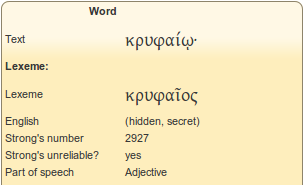
\includegraphics[width=0.4\textwidth]{unreliable.png}
\end{center}

\subsection{Feature: psp}

The \emph{psp} feature indicates the part of speech of the word. It is an enumeration features of
type \emph{psp\_t} and can have these values:

\begin{itemize}
\item adjective
\item adverb
\item aramaic
\item article
\item cond
\item conjunction
\item correlative\_or\_interrogative\_pronoun
\item correlative\_pronoun
\item demonstrative\_pronoun
\item hebrew
\item indefinite\_pronoun
\item interjection
\item interrogative\_pronoun
\item letter\_indeclinable
\item noun
\item noun\_other\_type\_indeclinable
\item numeral\_indeclinable
\item particle
\item personal\_pronoun
\item possessive\_pronoun
\item preposition
\item proper\_noun\_indeclinable
\item reciprocal\_pronoun
\item reflexive\_pronoun
\item relative\_pronoun
\item verb
\item NA (i.e., not applicable)
\end{itemize}

\subsection{Features: person, number, gender, case, and possessor\_number}

The \emph{person, number, gender,} and \emph{case} features indicate the person, number, gender, and
case of the word. They are enumeration features of type \emph{person\_t, number\_t, gender\_t,} and
\emph{case\_t,} respectively.

For possessive pronouns the \emph{number} feature indicates the number of the owned item, and the
\emph{possessor\_number} feature indicates the number of the owning item. The
\emph{possessor\_number} feature is an enumeration feature of type \emph{number\_t}.


The \emph{person\_t} enumeration has these values:

\begin{itemize}
\item first\_person
\item second\_person
\item third\_person
\item NA (i.e., not applicable)
\end{itemize}

The \emph{number\_t} enumeration has these values:

\begin{itemize}
\item singular
\item plural
\item NA (i.e., not applicable)
\end{itemize}

The \emph{gender\_t} enumeration has these values:

\begin{itemize}
\item masculine
\item feminine
\item neuter
\item NA (i.e., not applicable)
\end{itemize}

The \emph{case\_t} enumeration has these values:

\begin{itemize}
\item nominative
\item vocative
\item genitive
\item dative
\item accusative
\item NA (i.e., not applicable)
\end{itemize}

\subsection{Features: tense, voice, and mood}

The \emph{tense, voice,} and \emph{mood} features indicate the tense, voice, and
mood of a verb. They are enumeration features of type \emph{tense\_t, voice\_t,}
and \emph{mood\_t,} respectively.

The \emph{tense\_t} enumeration has these values:

\begin{itemize}
\item present
\item imperfect
\item future
\item second\_future
\item aorist
\item second\_aorist
\item perfect
\item second\_perfect
\item pluperfect
\item second\_pluperfect
\item NA (i.e., not applicable)
\end{itemize}

The \emph{voice\_t} enumeration has these values:

\begin{itemize}
\item active
\item middle
\item passive
\item middle\_or\_passive
\item middle\_deponent
\item passive\_deponent
\item middle\_or\_passive\_deponent
\item impersonal\_active
\item NA (i.e., not applicable)
\end{itemize}

The \emph{mood\_t} enumeration has these values:

\begin{itemize}
\item indicative
\item subjunctive
\item optative
\item imperative
\item infinitive
\item participle
\item imperative\_participle
\end{itemize}


\subsection{Feature: suffix}

The \emph{suffix} feature indicates the meaning of a word suffix. It is an enumeration features of
type \emph{suffix\_t} and can have these values:

\begin{itemize}
\item superlative
\item comparative
\item interrogative
\item negative
\item attic
\item particle\_attached
\item crasis
\item NA (i.e., not applicable)
\end{itemize}

\subsection{Feature: ref}

The \emph{ref} feature indicates the Bible verse to which this word belongs. For example, all words
in \bibleref{Luke}{2}{5} have the \emph{ref} feature set to ``Luke~2:5''.

\subsection{Features: form\_tag and functional\_tag}

The \emph{form\_tag} and \emph{functional\_tag} are taken directly from the original CSV file on
which this Emdros database is built. They are not used by Bible OL.

%%%%%%%%%%%%%%%%%%%% The sentence Object %%%%%%%%%%%%%%%%%%%%
\section{The \emph{sentence} Object}\index{sentence}

The \emph{sentence} object has no features. Its purpose is merely to group words.

%%%%%%%%%%%%%%%%%%%% The clause1 and clause2 Objects %%%%%%%%%%%%%%%%%%%%
\section{The \emph{clause1} and \emph{clause2} Objects}\index{clause1}\index{clause2}

The \emph{clause1} and \emph{clause2} objects have a single feature, \emph{typ.}

Although Bible OL only provides three levels of the syntax trees (\emph{sentence, clause1,} and
\emph{clause2}), the Syntax trees on which the database is based contain considerably more levels.
Adding more levels to Bible OL would require a completely different way to present the syntax trees,
and three levels are considered adequate for most cases.

\subsection{Feature: typ}

The \emph{typ} feature indicates the function of the clause. It is an enumeration features of
type \emph{clause\_type\_t} and can have these values:

\begin{my-tabu}{cl}{ \headii{Value}{Meaning} }
    ADV & Adverbial function       \\
    CL  & Clause                   \\
    IO  & Indirect object function \\
    O   & Object function          \\
    O2  & Second object function   \\
    P   & Predicate function       \\
    S   & Subject function         \\
    V   & Verbal function          \\
    VC  & Verbal copula function   \\
\end{my-tabu}


%%%%%%%%%%%%%%%%%%%% The Other Object Types %%%%%%%%%%%%%%%%%%%%
\section{The Other Object Types}

For information about the other object types in the nestle4 database, please consult the MQL code
used for generating the database. The MQL code can be seen by running the
\emph{mqldump}\index{mqldump} program as described on page \pageref{list-mqldump}.


%%%%%%%%%%%%%%%%%%%% The Origin of the Data %%%%%%%%%%%%%%%%%%%%
\section{The Origin of the Data}

The current Emdros database comes from three sources:

\begin{itemize}
\item A CSV file containing the text and grammar information, provided to me by Ulrik
  Sandborg-Petersen.\index{Sandborg-Petersen, Ulrik}
\item A lexicon derived from Jeff Dodson's Public Domain lexicon of the Greek NT, provided to me by
  Ulrik Sandborg-Petersen.
\item Syntax trees downloaded from\\
  \url{https://github.com/biblicalhumanities/greek-new-testament}.
\end{itemize}

The text and the lexicon are also available from \url{https://github.com/biblicalhumanities}.

The Emdros database has been created based on these sources using my program
\emph{nestle2mql,}\index{nestle2mql} which is currently not published or documented.

%%%%%%%%%%%%%%%%%%%%%%%%%%%%%%%%%%%%%%%%%%%%%%%
%%%%%%%%%%%%%%%%%%%% Index %%%%%%%%%%%%%%%%%%%%
\printindex

\end{document}

% Local Variables:
% mode: latex
% ispell-dictionary: "british-ize"
% ispell-extra-args: ("--home-dir=/home/claus/Projects/BibleOL/techdoc")
% eval: (auto-fill-mode 1)
% End:
